% Options for packages loaded elsewhere
\PassOptionsToPackage{unicode}{hyperref}
\PassOptionsToPackage{hyphens}{url}
%
\documentclass[
]{book}
\usepackage{amsmath,amssymb}
\usepackage{lmodern}
\usepackage{ifxetex,ifluatex}
\ifnum 0\ifxetex 1\fi\ifluatex 1\fi=0 % if pdftex
  \usepackage[T1]{fontenc}
  \usepackage[utf8]{inputenc}
  \usepackage{textcomp} % provide euro and other symbols
\else % if luatex or xetex
  \usepackage{unicode-math}
  \defaultfontfeatures{Scale=MatchLowercase}
  \defaultfontfeatures[\rmfamily]{Ligatures=TeX,Scale=1}
\fi
% Use upquote if available, for straight quotes in verbatim environments
\IfFileExists{upquote.sty}{\usepackage{upquote}}{}
\IfFileExists{microtype.sty}{% use microtype if available
  \usepackage[]{microtype}
  \UseMicrotypeSet[protrusion]{basicmath} % disable protrusion for tt fonts
}{}
\makeatletter
\@ifundefined{KOMAClassName}{% if non-KOMA class
  \IfFileExists{parskip.sty}{%
    \usepackage{parskip}
  }{% else
    \setlength{\parindent}{0pt}
    \setlength{\parskip}{6pt plus 2pt minus 1pt}}
}{% if KOMA class
  \KOMAoptions{parskip=half}}
\makeatother
\usepackage{xcolor}
\IfFileExists{xurl.sty}{\usepackage{xurl}}{} % add URL line breaks if available
\IfFileExists{bookmark.sty}{\usepackage{bookmark}}{\usepackage{hyperref}}
\hypersetup{
  pdftitle={BrailleR in Action},
  pdfauthor={A. Jonathan R. Godfrey},
  hidelinks,
  pdfcreator={LaTeX via pandoc}}
\urlstyle{same} % disable monospaced font for URLs
\usepackage{color}
\usepackage{fancyvrb}
\newcommand{\VerbBar}{|}
\newcommand{\VERB}{\Verb[commandchars=\\\{\}]}
\DefineVerbatimEnvironment{Highlighting}{Verbatim}{commandchars=\\\{\}}
% Add ',fontsize=\small' for more characters per line
\usepackage{framed}
\definecolor{shadecolor}{RGB}{248,248,248}
\newenvironment{Shaded}{\begin{snugshade}}{\end{snugshade}}
\newcommand{\AlertTok}[1]{\textcolor[rgb]{0.94,0.16,0.16}{#1}}
\newcommand{\AnnotationTok}[1]{\textcolor[rgb]{0.56,0.35,0.01}{\textbf{\textit{#1}}}}
\newcommand{\AttributeTok}[1]{\textcolor[rgb]{0.77,0.63,0.00}{#1}}
\newcommand{\BaseNTok}[1]{\textcolor[rgb]{0.00,0.00,0.81}{#1}}
\newcommand{\BuiltInTok}[1]{#1}
\newcommand{\CharTok}[1]{\textcolor[rgb]{0.31,0.60,0.02}{#1}}
\newcommand{\CommentTok}[1]{\textcolor[rgb]{0.56,0.35,0.01}{\textit{#1}}}
\newcommand{\CommentVarTok}[1]{\textcolor[rgb]{0.56,0.35,0.01}{\textbf{\textit{#1}}}}
\newcommand{\ConstantTok}[1]{\textcolor[rgb]{0.00,0.00,0.00}{#1}}
\newcommand{\ControlFlowTok}[1]{\textcolor[rgb]{0.13,0.29,0.53}{\textbf{#1}}}
\newcommand{\DataTypeTok}[1]{\textcolor[rgb]{0.13,0.29,0.53}{#1}}
\newcommand{\DecValTok}[1]{\textcolor[rgb]{0.00,0.00,0.81}{#1}}
\newcommand{\DocumentationTok}[1]{\textcolor[rgb]{0.56,0.35,0.01}{\textbf{\textit{#1}}}}
\newcommand{\ErrorTok}[1]{\textcolor[rgb]{0.64,0.00,0.00}{\textbf{#1}}}
\newcommand{\ExtensionTok}[1]{#1}
\newcommand{\FloatTok}[1]{\textcolor[rgb]{0.00,0.00,0.81}{#1}}
\newcommand{\FunctionTok}[1]{\textcolor[rgb]{0.00,0.00,0.00}{#1}}
\newcommand{\ImportTok}[1]{#1}
\newcommand{\InformationTok}[1]{\textcolor[rgb]{0.56,0.35,0.01}{\textbf{\textit{#1}}}}
\newcommand{\KeywordTok}[1]{\textcolor[rgb]{0.13,0.29,0.53}{\textbf{#1}}}
\newcommand{\NormalTok}[1]{#1}
\newcommand{\OperatorTok}[1]{\textcolor[rgb]{0.81,0.36,0.00}{\textbf{#1}}}
\newcommand{\OtherTok}[1]{\textcolor[rgb]{0.56,0.35,0.01}{#1}}
\newcommand{\PreprocessorTok}[1]{\textcolor[rgb]{0.56,0.35,0.01}{\textit{#1}}}
\newcommand{\RegionMarkerTok}[1]{#1}
\newcommand{\SpecialCharTok}[1]{\textcolor[rgb]{0.00,0.00,0.00}{#1}}
\newcommand{\SpecialStringTok}[1]{\textcolor[rgb]{0.31,0.60,0.02}{#1}}
\newcommand{\StringTok}[1]{\textcolor[rgb]{0.31,0.60,0.02}{#1}}
\newcommand{\VariableTok}[1]{\textcolor[rgb]{0.00,0.00,0.00}{#1}}
\newcommand{\VerbatimStringTok}[1]{\textcolor[rgb]{0.31,0.60,0.02}{#1}}
\newcommand{\WarningTok}[1]{\textcolor[rgb]{0.56,0.35,0.01}{\textbf{\textit{#1}}}}
\usepackage{longtable,booktabs,array}
\usepackage{calc} % for calculating minipage widths
% Correct order of tables after \paragraph or \subparagraph
\usepackage{etoolbox}
\makeatletter
\patchcmd\longtable{\par}{\if@noskipsec\mbox{}\fi\par}{}{}
\makeatother
% Allow footnotes in longtable head/foot
\IfFileExists{footnotehyper.sty}{\usepackage{footnotehyper}}{\usepackage{footnote}}
\makesavenoteenv{longtable}
\usepackage{graphicx}
\makeatletter
\def\maxwidth{\ifdim\Gin@nat@width>\linewidth\linewidth\else\Gin@nat@width\fi}
\def\maxheight{\ifdim\Gin@nat@height>\textheight\textheight\else\Gin@nat@height\fi}
\makeatother
% Scale images if necessary, so that they will not overflow the page
% margins by default, and it is still possible to overwrite the defaults
% using explicit options in \includegraphics[width, height, ...]{}
\setkeys{Gin}{width=\maxwidth,height=\maxheight,keepaspectratio}
% Set default figure placement to htbp
\makeatletter
\def\fps@figure{htbp}
\makeatother
\setlength{\emergencystretch}{3em} % prevent overfull lines
\providecommand{\tightlist}{%
  \setlength{\itemsep}{0pt}\setlength{\parskip}{0pt}}
\setcounter{secnumdepth}{5}
\usepackage{booktabs}
\ifluatex
  \usepackage{selnolig}  % disable illegal ligatures
\fi
\usepackage[]{natbib}
\bibliographystyle{apalike}

\title{BrailleR in Action}
\author{A. Jonathan R. Godfrey}
\date{2021-05-15}

\begin{document}
\maketitle

{
\setcounter{tocdepth}{1}
\tableofcontents
}
\hypertarget{preface}{%
\chapter*{Preface}\label{preface}}
\addcontentsline{toc}{chapter}{Preface}

If blind students are to truly gain access to statistical analyses, they will need to be able to successfully complete a course in statistics at university level. To do this, they must learn how the graphical techniques used in the sighted world look and are used. Generation of tactile images can show blind students what a particular graph does in a general sense, but greater understanding will come from generating these graphs as part of an analysis --- in the same way it does for sighted students.

While sighted students can make use of a number of graphical user interfaces (GUIs), blind students are restricted to use of the command-line mode of operation or typing out an R script in full. One key benefit of the GUI mode of working is the ability to quickly generate basic numerical and graphical analyses. Blind students need to gain the same information as their sighted peers without expending too much additional time and energy. The \texttt{BrailleR} package aims to bridge this gap by delivering the range of analyses commonly found in introductory courses via a reduced set of commands.

Once blind students have completed their first course in statistics, they may embark on research at a university, or head out into industry to apply their knowledge. Irrespective of the direction they choose, they will need certainty in being able to independently create graphs for the sighted readers of their work.
Creation of tactile images that provide the same representation of the images to be placed in documents can provide a solution, but all too often blind people do not have access to the right software and hardware to generate tactile images for themselves with the immediacy that is required. The \texttt{BrailleR} package aims to provide textual information to the blind user in conjunction with the graph that would be placed in the final report. \texttt{BrailleR} does this by interpreting the object that is implicitly created whenever a graph is created in R. by creating an appropriate and concise text representation of the graph.

In summary, this book presents the work included in the \texttt{BrailleR} package that will assist blind students successfully complete an introductory course in statistics when other software options fail them. Many of the functions support workflows that improve the efficiency of blind users at all levels of experience.

I've tried a few ways to help get blind people using the BrailleR package and needed a place to combine the efforts easily. I don't yet know if this e-book will turn into anything but a few webpages, but let's see shall we?

Jonathan Godfrey

\hypertarget{citation-details}{%
\subsection*{Citation details}\label{citation-details}}
\addcontentsline{toc}{subsection}{Citation details}

Please refer interested parties to the online edition of this work at \url{https://R-Resources.massey.ac.nz/BrailleRInAction/}

When citing this work, please use the title, author, and date information on this page. The online version has ISBN978-0-473-41495-5 and is preferred for citation over other formats. The epub version has ISBN 978-0-473-41493-1 and pdf version has ISBN 978-0-473-41494-8; these fixed formats were created in October 2017.

\hypertarget{copyright-information}{%
\subsection*{Copyright information}\label{copyright-information}}
\addcontentsline{toc}{subsection}{Copyright information}

This work is licensed under the Creative Commons Attribution-NonCommercial-NoDerivatives 4.0 International License. To view a copy of this license, visit \url{http://creativecommons.org/licenses/by-nc-nd/4.0/} or send a letter to Creative Commons, PO Box 1866, Mountain View, CA 94042, USA.

\hypertarget{introduction}{%
\chapter{Introduction}\label{introduction}}

Access to information is crucial for a blind person's success in education, but transferring the knowledge about the existence of techniques into actually being able to perform those tasks is what will make that blind person employable. This e-book is based on the author's experiences as a blind academic in statistics who has often been called on for advice by blind students studying statistics and their sighted lecturers wanting to provide the best possible support. Unfortunately, there is little information available in academic journals or the public domain to offer the statistics lecturer who is about to teach a blind student for the first time. That is changing however.

At the 2009 Workshop on E-Inclusion in Mathematics and Sciences, I was able to meet other researchers and scientists who are also concerned about the low rate of blind people entering the sciences in a broad sense and the mathematical sciences in particular. \citep{Godfrey2009AccessiblePaper} presented my first formalized summary of what I saw as the current state of affairs for blind people taking statistics courses; that work discussed what was possible in theory, but lacked evidence of what was happening in practice.
A collaboration with the only other blind person to gain employment as a full-time Lecturer in Statistics led to a more comprehensive review of what we believe is the current state of affairs for blind students learning statistics. \citep{GodfreyLoots-JSE} present a wide range of issues that blind students and their teachers must overcome, often through use of the best software options available today. R \citep{Rpkg-base} has featured as a key element in my recommendations for teaching statistics to blind students \citep{Godfrey2009AccessiblePaper} because it offers the greatest opportunity for meeting the needs of blind users.

An invitation to attend the \href{http://icchp-su.net/}{second ``Summer University'' event} was taken up in mid 2011; the purpose of this event was to show blind students and disability support staff from universities what software and hardware is available to improve the success rates of blind students entering the sciences.
This was my first direct opportunity to show blind students how R could be used by them, and the relative merit that R has for them over alternative statistical software.
I observed blind students working with R and struggling more than I thought was truly necessary. I knew I could do something about it and have spent a lot of time doing so ever since.
An R Journal article \citep{GodfreyRJournal} followed which exposed the needs of blind users to the R community and also announced the initial development of the \texttt{BrailleR} package \citep{Rpkg-BrailleR}.

The \texttt{BrailleR} package is my attempt to help blind students and their lecturers. It is built on functions that I use to work as a lecturer in statistics. It aims to make up for the inability blind users have to work with the same extension tools their sighted peers are using, including the increasing number of graphical user interface (GUI) and integrated development environment (IDE) options.

\hypertarget{why-will-i-use-the-brailler-package-as-a-novice}{%
\section{Why will I use the BrailleR package as a novice?}\label{why-will-i-use-the-brailler-package-as-a-novice}}

Blind users will want to use the BrailleR package while they are novice R users, but may also want to continue using some of the tools as their skill levels increase. Each of the following reasons for using the BrailleR package are expanded on by way of examples that go into more detail in subsequent chapters of this text.

\hypertarget{brailler-improves-the-accessibility-of-graphical-information}{%
\subsection{BrailleR improves the accessibility of graphical information}\label{brailler-improves-the-accessibility-of-graphical-information}}

BrailleR converts standard graphs created by standard R commands into a textual form that can
be interpreted by blind students who cannot access the graphs without
printing the image to a tactile embosser, or who need the extra text to
support any tactile images they do create.

At present this is limited to only a few graph types found in base R functionality. An example of a histogram is presented in Chapter \ref{VI}.

\hypertarget{brailler-helps-gain-access-to-the-content-of-the-r-console}{%
\subsection{BrailleR helps gain access to the content of the R console}\label{brailler-helps-gain-access-to-the-content-of-the-r-console}}

BrailleR makes text output (that is
visually appealing) more useful for a blind user who is reliant on
synthesized speech or braille output to interpret the results. The first example of this kind presented in Chapter \ref{VI} shows how the summary statistics for a dataset can be made easier for a screen reader user.

\hypertarget{brailler-includes-convenience-functions}{%
\subsection{BrailleR includes convenience functions}\label{brailler-includes-convenience-functions}}

Many analyses get repeated over and over again with different variables. Some people like a graphical user interface (GUI) but none of the GUIs developed for R to date are accessible by screen reader users.

BrailleR includes some functions which generate pro forma analyses. When these functions are employed, they generate an HTML document that includes the analysis in an easy to use format. The R commands used to create the analysis are stored in an R script file so that a user can modify the commands if changes are necessary. These functions are introduced in Chapter \ref{RMarkdown}.

\hypertarget{why-will-i-use-the-brailler-package-if-i-am-not-a-novice}{%
\section{Why will I use the BrailleR package if I am not a novice?}\label{why-will-i-use-the-brailler-package-if-i-am-not-a-novice}}

I think some of the reasons for using the package while you are a novice R user remain relevant to more-experienced users too, but perhaps the main reason for continuing to use BrailleR is that of efficiency.
The convenience functions introduced in Chapter \ref{RMarkdown} give you a starting point for analyses. Behind those convenience functions was an R markdown file that generated the R script and the HTML document. Getting into markdown is a great idea and will not take you long to learn.

BrailleR also includes some tools for helping run your R jobs without running R. Experienced users do this all the time so these tools aren't really meant for blind users alone, but as blind people often find little inefficiencies tiresome, I've incorporated the tools I use for my own efficiency when I think they might prove useful to other blind people.

In summary, the \texttt{BrailleR} package is my attempt to help blind students and their lecturers. It is built on functions that I use to work as a lecturer in statistics. It aims to make up for the inability blind users have to work with the same extension tools their sighted peers are using, including the increasing reliance on GUIs and integrated development environment (IDE) options.

\hypertarget{why-will-i-use-this-book}{%
\section{Why will I use this book?}\label{why-will-i-use-this-book}}

This book has been compiled for a variety of reasons. The obvious reason is that the \texttt{BrailleR} package has many tools that cannot be demonstrated using the standard documentation options found in many packages. Some of the material found here did start in package vignettes, but the time taken to re-work them all was slowing down development of the package.

A key feature of this book is that it was written by a blind person, using only the tools the book suggests, to create a book that can be read by blind people. This end to end workflow is proof that the \texttt{BrailleR} package helps make some actions possible, and others easier for a blind person to undertake. All too often, blind people find themselves using substitute workflows that are painfully slow compared to the tools being used by our sighted peers. I'm not suggesting that the tools here will make a blind person more efficient than all of their peers, but being able to use the most efficient tools that sighted people could choose to use does matter. Using these tools will cut the disadvantage a blind person has to a minimum; I'd even go so far as to suggest that the gap between a blind person and a sighted person's efficiency is reduced if we use the best tools on offer as compared to the gap we'd suffer if we chose to use inferior tools.

\hypertarget{what-this-book-is-not}{%
\section{What this book is not}\label{what-this-book-is-not}}

This book is not a comprehensive guide to using R. There are now hundreds of books a blind (or sighted) person could choose to wade through, some are good, some are great, and some are truly awesome! There are also plenty of resources on the internet that are tired and really should be avoided. I am keen to promote those texts that can be easily worked with by a blind user. I'll mention them as we get to the right point in this book for doing so, but now is a good time to mention a few that have really made a difference to me and creation of this book.

I am truly reliant on the resources offered by help pages hosted by RStudio. I often include RStudio.com in my list of search terms. In adition, many of the individuals I hold in very high regard have close ties to RStudio.

Yihui Xie's work on the \texttt{knitr} package \citep{Rpkg-knitr}
and his books on writing documents using reproducible research techniques \citep{Xie2015}
are key to my success and in my opinion, have also led to making life much easier for blind users to read the work of others and to create new content for themselves.

I frequently use several books written by Hadley Wickham and his collaborators. In particular, I rate the \href{http://r-pkgs.had.co.nz/}{R packages book} \citep{Wickham2015RPackages}, the \href{https://adv-r.hadley.nz}{Advanced R book} {[}\citet{Wickham2014Advanced}', and the \href{http://r4ds.had.co.nz/}{R for Data Science book} \citep{GrolemundWickham2016}.

\hypertarget{History}{%
\chapter{History of the BrailleR Project}\label{History}}

I am one of only two blind people in the world today who gained employment as full-time lecturers of statistics, that is, teaching statistics classes and doing research in theoretical matters as against applying statistical techniques. For years, I tried to keep my blindness separate from my research but I took some opportunities that came my way and heeded the advice of some colleagues to put more energy into improving the ability of blind students around the world to have greater access to statistics courses and statistical understanding. This document shows you a bit more insight into how I (with the help of some useful collaborations) got the BrailleR package to where it is now.

\hypertarget{my-background}{%
\section{My background}\label{my-background}}

My adult life has been centred around Massey University, initially as an extramural student and then studying on campus. I have undergraduate degrees in Finance and Operations Research, a Master's degree in Operations Research and a PhD in Statistics. I was a Graduate Assistant from 1998 to 2002, and then Assistant Lecturer from January 2003 to June 2004 when I became a Lecturer in Statistics. I was promoted to Senior Lecturer in late 2014.

While I don't find it important, I do get asked about the condition that caused my blindness. It is Retinitis Pigmentosa. I do have some light perception, and can make use of it in familiar surroundings for orientation but it has no value to me for reading anything at all. I chose to work with screen reading software when I started university and obtained my first computer because my residual vision at the time was limiting my reading speed. I have therefore operated a computer as a totally blind user throughout my adult life.

I did not learn braille until after I completed my PhD. This might seem strange, but there was very little material in a suitable digital format for me to read throughout my student life. Things have changed and I now spend a lot more time reading material and doing programming where the accuracy of braille is absolutely necessary. Braille has now become a very important part of my working life and I have a braille display connected to my computer most of the time.

\hypertarget{getting-the-brailler-project-started}{%
\section{Getting the BrailleR Project started}\label{getting-the-brailler-project-started}}

I used to keep my research interests separate from my blindness, but I was regularly called upon to discuss how a blind person could study and teach Statistics by many people within New Zealand and occasionally from overseas. In 2009, I attended the Workshop on E-Inclusion in Mathematics and Science (WEIMS09) where I met other people interested in improving the success rates of blind students in the mathematical sciences. My paper was about accessibility of statistics courses, but I did point out the usefulness of R in preference to other tools I had used to that point in time \citep{Godfrey2009AccessiblePaper}.

I discovered that there is room for me to take a leading role in the development of ideas that can help other blind people learn about statistical concepts. I have been invited to all six Summer University events run by the organizers of the International Conference on Computers Helping People (ICCHP), but have been unable to attend twice due to the high cost of transporting me to Europe. I have delivered an introductory workshop on using R at four of these events \citetext{\citealp{Godfrey2011SU-R}; \citealp{Godfrey2013SU-R}; \citealp{Godfrey2014SU-R}; \citealp[and][]{Godfrey2016SU-R}}.

Having observed the attendees at the 2011 Summer University as they came to grips with R, I knew there was more I could do to help them and other blind students. I started work on the BrailleR package \citep{Rpkg-BrailleR} in the second half of 2011 and first proposed it could work for blind users at the Digitisation and E-Inclusion in Mathematics and Science (DEIMS12) workshop held in Tokyo during February 2012 \citep{Godfrey2012BrailleRPaper}.

I wasn't to know the value of another talk I gave at DEIMS12 for another two years; this second talk and associated conference paper focused on how I was using Sweave to create accessible statistical reports for me and more beautifully formatted ones for my statistical consulting clients.
\citep{Godfrey2012PuttingPaper}. I now know that the groundwork I had done contributed to my desire to present my workflow as a workshop at the 5\textsuperscript{th} Summer University in 2014 \citep{Godfrey2014SU-Sweave}.
It also stood me in good stead for the work that followed on the \texttt{BrailleR} package as it developed in late 2014 and early 2015.

\hypertarget{the-starting-point-example}{%
\section{The starting point example}\label{the-starting-point-example}}

The basic graph that has been used for almost every presentation of the \texttt{BrailleR} package is a histogram. There is a more detailed example, but the following commands create a set of numbers that can be kept for further processing once the graph has been created. It is the re-processing of these numbers that leads to the text description that follows.

\begin{Shaded}
\begin{Highlighting}[]
\FunctionTok{library}\NormalTok{(BrailleR)}
\end{Highlighting}
\end{Shaded}

\begin{verbatim}
## The BrailleR.View,  option is set to FALSE.
\end{verbatim}

\begin{verbatim}
## 
## Attaching package: 'BrailleR'
\end{verbatim}

\begin{verbatim}
## The following objects are masked from 'package:graphics':
## 
##     boxplot, hist
\end{verbatim}

\begin{verbatim}
## The following object is masked from 'package:utils':
## 
##     history
\end{verbatim}

\begin{verbatim}
## The following objects are masked from 'package:base':
## 
##     grep, gsub
\end{verbatim}

\begin{Shaded}
\begin{Highlighting}[]
\NormalTok{x}\OtherTok{=}\FunctionTok{rnorm}\NormalTok{(}\DecValTok{1000}\NormalTok{)}
\FunctionTok{VI}\NormalTok{(}\FunctionTok{hist}\NormalTok{(x))}
\end{Highlighting}
\end{Shaded}

\begin{figure}
\centering
\includegraphics{02-History_files/figure-latex/hist-1.pdf}
\caption{\label{fig:hist}A histogram of 1000 random values from a normal distribution}
\end{figure}

\begin{verbatim}
## This is a histogram, with the title: Histogram of x
## "x" is marked on the x-axis.
## Tick marks for the x-axis are at: -4, -2, 0, and 2 
## There are a total of 1000 elements for this variable.
## Tick marks for the y-axis are at: 0, 50, 100, 150, and 200 
## It has 15 bins with equal widths, starting at -4 and ending at 3.5 .
## The mids and counts for the bins are:
## mid = -3.75  count = 1 
## mid = -3.25  count = 1 
## mid = -2.75  count = 5 
## mid = -2.25  count = 9 
## mid = -1.75  count = 44 
## mid = -1.25  count = 96 
## mid = -0.75  count = 159 
## mid = -0.25  count = 185 
## mid = 0.25  count = 194 
## mid = 0.75  count = 143 
## mid = 1.25  count = 106 
## mid = 1.75  count = 39 
## mid = 2.25  count = 12 
## mid = 2.75  count = 4 
## mid = 3.25  count = 2
\end{verbatim}

This first example showed me what was possible if only I could get a few things sorted out. All histograms are created by a function that stores the results (both numeric and text details) and calls this stored set of values a ``histogram''. The main issue is that storing the set of details is not consistent in R, nor is the fact that the stored object gets given a ``class'' to tell me what type of object it is. This problem haunted me for quite some time because I was talking to the wrong people about the problem; it was time to find people that held the solution instead of talking to the people that would benefit if a solution was found.

\hypertarget{why-just-plain-text}{%
\section{Why just plain text?}\label{why-just-plain-text}}

The first initiative of \texttt{BrailleR} was to turn information presented in a visual medium into a medium that is simple to work with, efficient, and complementary to the skill set of as wide a group of blind people as possible. With this in mind, a plain text solution for gaining access to visual information was favoured above tactile images as there is no need for any additional adaptive technology (hardware or software) over that used for the blind person's other work.
Information presented in text is readable in braille or heard via synthetic speech, and is therefore only limited to the user's skill set.

Other research projects are progressing the creation of tactile images that replace the printed graphics sighted people deal with all the time in statistical work. Tactile images do have a role to play in educating blind people and providing them with access to information, but their greatest drawback remains their lack of immediacy. Rendering a graphic into a master file complete with braille labels, and then producing this for consumption are tasks receiving much attention, but the value for such efforts is probably greatest for situations where one master can be used to create multiple copies for wider consumption such as the conversion of textbooks into braille. Some preliminary investigations into the ability to create tactile image versions of graphs created in R have been made as part of the wider BrailleR Project.

Under a sighted paradigm, many graphs in statistical work are developed for one-time use and discarded almost immediately.
It may be some time until the effectiveness of tactile image hardware and software is ready to deliver this outcome for all blind users of R; in the meantime, we must find ways of gaining access to the graphical information without reliance on another person's ability to translate the visual medium into something more useful for us. We must also acknowledge here that the number of blind people with their own tactile image hardware and software is regrettably low. Even though it is possible to directly export a graph created in R to an embosser, use of this practice is not yet commonplace.
Perhaps we can look forward to the time when most blind people can have access to a refreshable tactile display that can display two-dimensional images that compare with the best that is possible in hard copy today.

Sonification is considered by many to be an alternative to production of tactile images for a blind audience. Work on sonifying statistical graphs is being considered, but is at present best described as experimental. Several concerns must be overcome before sonification can be claimed a truly useful method for interpretting data. There is an assumption made frequently by correspondents with this author that lack of vision implies a blind person has superior aural ability . This may be true for some blind people, but it is not universally true. We must be sure that the interpretation gained through sound is comparable to the interpretation that a graph in visual form would convey. Proponents of sonification often suggest that sound provides a different interpretation to a visual display. If they are correct, then sonification cannot be a true alternative to a visual graph. The same, of course, can be said for the difference between the interpretation obtained through touching tactile images. In both cases, the solution for blind users must be that the visual representation can be converted to a useful format when blind users need it, without the assistance of a sighted person to check the validity of the outcome.

\hypertarget{exposure-of-the-brailler-package-outside-the-blind-community}{%
\section{Exposure of the BrailleR package outside the blind community}\label{exposure-of-the-brailler-package-outside-the-blind-community}}

It was obvious to me that getting the word out to the masses about the usefulness of R for blind students and professionals was crucial. I started to compile my notes built up from various posts made to email groups and individuals over the years, as well as the lessons I learned from attendance at the 2\textsuperscript{nd} Summer University event. This led to the eventual publication of my findings in \citep{GodfreyRJournal}. I know that this was a worthwhile task because it was read by teachers of blind students who were already using R for their courses. One such person tested R and a screen reader and managed to find a solution to a problem posed in \citet{GodfreyRJournal} which led to an addendum \citep{GodfreyErhardtRJournalAddendum}.

I presented some of my work via a poster \citep{Godfrey2013BlindnessPoster} at the NZ Statistical Association conference in Hamilton during November 2013. This `poster' presentation was developed as a multimedia presentation so that the audience could observe video footage, handle tactile images and be able to talk with me about the BrailleR Project. The plan to get talking with people instead of talking at them worked and I started a really useful collaboration with Paul Murrell from the University of Auckland. His major contributions didn't feature in the BrailleR package for some time, but we're making some really nice progress. Paul is an expert in graphics, especially their creation and manipulation in R. Our discussions about graphics has yielded a few titbits for my own work that have been tested for the package. We've been working on how to make scalable vector graphics that can be augmented to offer blind users greater interactivity and therefore hopefully greater understanding \citep[see][]{GodfreyMurrell2016TactileGraphsPaper}.

\hypertarget{reviewing-statistical-software}{%
\section{Reviewing statistical software}\label{reviewing-statistical-software}}

I have been asked about the use of R in preference to other statistical software by many blind students, their support staff, and their teachers.
Eventually I joined forces with the only other blind person to gain employment as a lecturer of statistics (Theodor Loots, University of Pretoria) to compare the most commonly used statistical software for its accessibility \citep{GodfreyLoots2014JSS}.
I summarised this paper at the 5\textsuperscript{th} Summer University event \citep{Godfrey2014SU-StatsSoft}, and offered a similar presentation at the 6\textsuperscript{th} Summer University event \citep{Godfrey2016SU-StatsSoft} with a few updates.
It is important to keep abreast of developments, because the statistical software changes, and so does the screen reading software that gives us access to the mainstream statistical software.

\hypertarget{attendance-at-user-conferences}{%
\section{Attendance at UseR conferences}\label{attendance-at-user-conferences}}

On my way to the 5\textsuperscript{th} Summer University event, I managed to attend the principal conference for R users (UseR!2014) in Los Angeles where I presented my findings \citep{Godfrey2014BlindUseROral}.
Perhaps the most valuable outcome of this conference was the ability to attend a tutorial on use of the \texttt{knitr} package \citep{Rpkg-knitr} and then talk to its author, Yihui Xie.
I'd already seen the \texttt{knitr} package before attending UseR!2014 and implemented it for some of my teaching material by updating the Sweave documents already in use.\\
The real value came in realising what I could probably do if I used R markdown to do a few things I had found very hard using the Sweave way of working.
More specifically, generating an R markdown file (Rmd) from an R script was much easier than generating a Sweave file (Rnw).
Writing the convenience functions for the \texttt{BrailleR} package started to look very achievable at this point, and so work began.
I dug out some old work that wasn't fit for sharing and converted it to the markdown way of working.
There has been sufficient progress in the BrailleR Project that I presented it at UseR!2015 \citep{Godfrey2015BaseRWeepsOral}. In 2016, I presented my findings on writing (and therefore reading) R markdown documents for (and by) blind users \citep{GodfreyBilton2016UseROral}.

\hypertarget{the-ongoing-work}{%
\section{The ongoing work}\label{the-ongoing-work}}

The introduction of R markdown to the BrailleR package made a huge difference.
I've been able to write enough example code that once I found a friendly postgraduate student (Timothy Bilton) to put some time into it, we've managed to add more convenience functionality.
Timothy improved some of my earlier work and tried a few things of his own.
This left me with the time to add increased functionality for helping blind users get into markdown for themselves.

One of my irritations of working with markdown is that everyone else seems to write markdown and check their findings using RStudio \citep{RStudio}, which remains inaccessible for me and other screen reader users. I took an old experiment where I wrote an accessible text editor in wxPython, and with the help of a postgraduate student from Computer Science (James Curtis) we've modified it to process Rmd files.
The \texttt{WriteR} application is now beyond experimental but there is still more to do on making it truly useful \citep{GodfreyCurtis2016WriteRPaper}.
In 2018, I received a great deal of assistance from Marshall Flax who was able to help develop \texttt{WriteR} into a tool that could be very useful to blind people wishing to write and process R markdown files.

\hypertarget{acknowledgements}{%
\section{Acknowledgements}\label{acknowledgements}}

Contributions to the BrailleR Project are welcome from anyone who has an
interest. I will acknowledge assistance in chronological order of the
contributions I have received thus far.

Greg Snow was the first person to assist when he gave me copies of the
original R code and help files for the R2txt functions that were part of
his \texttt{TeachingDemos} package \citep{Rpkg-TeachingDemos}.

The Lions clubs of Karlsruhe supported my attendance at the 3\textsuperscript{rd} Summer
University event in 2013. This gave me the first opportunity to
put the package in front of an audience that I hope will gain from the
package's existence.

I've already mentioned the following contributors above:Paul Murrell, Yihui Xie, Timothy Bilton, James Curtis, and Marshall Flax.

I also need to acknowledge the value of attending the Summer University events. I gain so much from my interactions with the students who attend, the other workshop leaders who give me feedback, and the other professionals who assist blind students in their own countries.

\hypertarget{GettingStarted}{%
\chapter{Getting started with BrailleR}\label{GettingStarted}}

The BrailleR package has been created for the benefit of blind people wishing to
get more out of R than it already offers --- which is actually quite a
lot!

\hypertarget{accessibility-of-statistical-software}{%
\section{Accessibility of statistical software}\label{accessibility-of-statistical-software}}

A description of what makes statistical software accessible to the blind was given by \citep{GodfreyLoots2014JSS}. Many of the problems blind people face are a consequence of the failure of the specialist screen reading software we use to interact with graphical user interfaces.
Many software applications are making use of graphics when once the information would be presented in text form with an accompanying graph. --- SPSS \citep{SPSS-Soft} is an example of this, and to a lesser extent so is the standard edition of Minitab \citep{Minitab-Soft}. The output from Minitab Express \citep{Minitab-Express} is a prime example of the worst possible presentation of information that was originally text; this product generates graphics that include text which is not readable by a blind person for all of its statistical output. The speech output software used by blind people can only interpret information that is text. As a guide, if the individual text in a window cannot be highlighted using the keyboard and not the mouse, then it is likely that this text will not be read for the blind user.

It is true that some add-on packages for R also generate unreadable output, but as illustrated below, this is less of an issue than for software like SPSS or Minitab.
\citep{GodfreyLoots2014JSS} gave more detailed scrutiny of R, SAS \citep{SAS-Soft} , SPSS, and Minitab. Of these four applications, R and SAS were clearly superior to SPSS and the standard edition of Minitab.

Some software applications have retained their historical links to the days when graphs and tables were rendered in well controlled monospace fonts --- Minitab for example. In such applications the user may still be able to produce an ASCII graphic instead of the more commonly used high resolution graphs expected of today's software (and user). In contrast, SAS and SPSS can use HTML to present information in well-formatted tables. These output windows are preferred by blind users over the graph window displays but sometimes the amount of information is not easily understood. Presentation of output is often read by eye in a vertical direction, while speech output software will read line by line. Take for example, a multiple regression where the sighted reader may scan down the list of \emph{p} values in the right hand column; the same information being read aloud in line by line style could prove quite difficult to interpret. Blind users can use combinations of keys to move around HTML tables to speed up this process and avoid reading the intervening columns of output. While SPSS and SAS can deliver formatted HTML as a matter of course, R users must resort to the add-on packages, many of which are available on CRAN.

\hypertarget{accessibility-of-r}{%
\section{Accessibility of R}\label{accessibility-of-r}}

\citep{GodfreyRJournal} documented the ability to use R almost immediately after installation; only one minor change is recommended and can be achieved in less than a minute even when explained via email or a telephone call. For users of the Windows operating system, up until Windows XP, I always recommended running R in a terminal window instead of the GUI; the shortcut placed on the Windows desktop would then need to be pointed to \texttt{Rterm.exe} instead of \texttt{Rgui.exe}.
Macintosh and Linux users are operational with no special actions required.
Users of Windows Vista or Windows 7 did have an additional challenge of what appeared to be the screen locking up, or more exactly, the screen reader software ``losing focus'' in the R terminal window. The solution for this problem, as documented in \citep{GodfreyErhardtRJournalAddendum}, was to hit the \texttt{Alt} key.
Blind users now need to compare the combinations of screen reader and the terminal versus the GUI.
The decision should be made by the individual user after some experimentation; their decision may depend on the skill level they have with their prefered screen reader and should be revisited at a later date.

Blind students attending the \href{http://icchp-su.net/?q=node/108}{R workshop at the 2011 Summer University,} held in the Czech Republic, were able to set up R for use in a classroom setting on their own machines. This included a variety of operating systems and adaptive technology (hardware and software for blind people). Similar events were held in 2013 and 2014 but most attendees used computers supplied by the host organizing committees. Many attendees have made contact when issues have arisen, but none of the issues relate to the installation of R or its interactions with the particular hardware or software being used. I am confident that anyone intending to undertake use of any statistical software will be able to get R working with their screen reader.

\hypertarget{installing-the-brailler-package}{%
\section{Installing the BrailleR package}\label{installing-the-brailler-package}}

To use the functionality of the BrailleR package you need to have it installed. The package has several dependencies so installation from the CRAN repository is recommended. This would be done by issuing the following two commands in an R session:

\begin{Shaded}
\begin{Highlighting}[]
\FunctionTok{chooseCRANmirror}\NormalTok{(}\AttributeTok{ind=}\DecValTok{1}\NormalTok{)}
\FunctionTok{install.packages}\NormalTok{(}\StringTok{"BrailleR"}\NormalTok{)}
\end{Highlighting}
\end{Shaded}

Note that the first and last letters of \texttt{BrailleR} are capitalised. This is important in R, but is also useful for screen reading software which will then give audibly different feedback, as compared to what a screen reader user hears from the lower case text ``brailler''.

If for some reason you have difficulty with the above commands, you can install the BrailleR package using a zip file version available from a CRAN repository or the latest version on GitHub.

From time to time, you should check that you are using the most recent version of the BrailleR package. You can update all installed packages using the commands:

\begin{Shaded}
\begin{Highlighting}[]
\FunctionTok{chooseCRANmirror}\NormalTok{(}\AttributeTok{ind=}\DecValTok{1}\NormalTok{)}
\FunctionTok{update.packages}\NormalTok{(}\AttributeTok{ask=}\ConstantTok{FALSE}\NormalTok{)}
\end{Highlighting}
\end{Shaded}

Once you've got the package installed, you still need to get it running in your current R session by issuing one last command. When you issue the first of the following lines, the package start messages will also appear.

\begin{Shaded}
\begin{Highlighting}[]
\FunctionTok{library}\NormalTok{(BrailleR)}
\end{Highlighting}
\end{Shaded}

You're ready to go!

\hypertarget{some-initial-setting-up-instructions}{%
\subsection{Some initial setting up instructions}\label{some-initial-setting-up-instructions}}

When you first use the \texttt{library(BrailleR)} command, you will see some start up messages and a question. The rules of R packages include not writing to the user's hard drive without expressly asking them for permission to do so. If you do not want a folder for your \texttt{BrailleR} files then use the temporary folder which will be removed when you end your R session. This will mean you need to answer the question over the location of the \texttt{MyBrailleR} folder next time you issue the \texttt{library(BrailleR)} command though.

The welcome message from \texttt{BrailleR} suggests you issue the \texttt{GetGoing()} command. This will ask you a few questions that will help personalise your use of the \texttt{BrailleR} package. We will see how to alter these settings in Chapter \ref{Personalising} later so don't panic if you don't do it all right the first time. You can re-issue the \texttt{GetGoing()} command again at any time.

The book you are reading now can be reached from your R session by issuing the command \texttt{BrailleRInAction()}. That might seem a bit much, but do remember you can use tab completion to avoid typing the whole command name out in full. You will probably need no more than \texttt{B}, \texttt{r}, \texttt{a}, then tab (which adds the rest of BrailleR), then \texttt{I} and one last tab; add the opening and closing parentheses and press the Enter key. This will open the front page of the book in your browser. A similar command, \texttt{BrailleRHome()}, will open the BrailleR Project home page. You will need to be careful with upper versus lower case when entering commands. Note that there are often capitalised letters in the middle of \texttt{BrailleR} commands. This is known as ``camel case'' and it works well for screen reader users.

It is all too easy to feel you're doing it on your own, which even the most accomplished people have experienced. I put the \texttt{ThankYou()} command in the BrailleR package so that it would be easy to send me a message to tell me about your experiences as a blind person using R or to ask for help; it starts an email message to me. I'm not the only blind person out there using R, and many of us are on an email list so that we can share ideas and solutions for problems, many of which are specific to blind users. The \texttt{JoinBlindRUG()} command will start the email needed to join the BlindRUG email list.

\hypertarget{what-else-do-you-need}{%
\section{What else do you need?}\label{what-else-do-you-need}}

You obviously have R installed or an intention to do so soon if you are reading this document. Aside from R and the add-on packages that BrailleR needs, there are no other software requirements. There are several optional software installations that could make life easier if they are installed before you need them. In order of necessity, they are:

\hypertarget{the-document-converter-pandoc}{%
\subsection{The document converter --- pandoc}\label{the-document-converter-pandoc}}

BrailleR requires the very useful file converter called pandoc. Get it from the
\href{https://github.com/jgm/pandoc/releases}{pandoc download page}

\hypertarget{the-principal-integrated-development-environment-rstudio}{%
\subsection{The principal integrated development environment --- RStudio}\label{the-principal-integrated-development-environment-rstudio}}

It is a good idea to install RStudio, even if you can't actually use it as a blind person using screen reading software. The reason is that RStudio installs a few other useful tools that we will make use of by other means. Get it from the
\href{https://www.rstudio.com/products/rstudio/download2}{RStudio download page}

\hypertarget{one-programming-language-python}{%
\subsection{One programming language --- Python}\label{one-programming-language-python}}

WriteR is a simple text editor written in wxPython that needs Python and wxPython. Unfortunately, they require separate downloads. You do not need this editor so do not install Python unless you are really keen. Windows users can obtain an executable file by issuing \texttt{GetWriteR()} once the BrailleR package has been successfully installed. More on this in Chapter \ref{WriteR}.

\hypertarget{brailler-commands-used-in-this-chapter}{%
\section{BrailleR commands used in this chapter}\label{brailler-commands-used-in-this-chapter}}

The only BrailleR command actually recommended in this chapter was \texttt{GetGoing()}. You might find it useful to use \texttt{BrailleRHome()} and \texttt{BrailleRInAction()} from time to time, but you're already reading the book that the second of these commands opens.

The \texttt{ThankYou()} and \texttt{JoinBlindRUG()} commands should be used when you want to connect with me, or other blind R users.

At this stage it is recommended that you install any additional software manually when it is required.

\hypertarget{VI}{%
\chapter{Some basic examples}\label{VI}}

This chapter presents some examples of text output generated by the \texttt{VI()} command of the \texttt{BrailleR} package. These examples generate output that is displayed in the R session just like any output from standard R commands. Please note however that not all \texttt{VI()} commands behave in this fashion; some more advanced uses of \texttt{VI()} are discussed in later chapters.

You will need the \texttt{BrailleR} package to be ready for use to follow along with the examples in this chapter. Do this by issuing the command \texttt{library(BrailleR)} now.

\hypertarget{accessibility-of-graphics-in-statistical-software}{%
\section{Accessibility of graphics in statistical software}\label{accessibility-of-graphics-in-statistical-software}}

Access to graphical representations of information from mathematical or statistical software is quite limited, and therefore limits the blind user's capacity. To this author's knowledge, no mathematical or statistical software has the capability of directly linking to any hardware or software solutions that make the information presented in graphs immediately available. The scalable vector graphic (SVG) format can be used to present a graphic with text embedded into the file for creating access for a blind user \citep{BulatovGardner2004SVG, GardnerBulatov2010SVG}.
Only a small number of statistical software applications have the capacity to create SVG files, but this capacity does not in itself create access because the text that makes them accessible must be added somehow; generally this is a manual process. The World Wide Web Consortium has a recommendation on the use of SVGs in web content \citep{SVGStandard} and a number of add-on packages for R make use of SVG because of the opportunity to enrich a graphic's interactivity in webpages; see \citep{MurrellPotter2014} for a more detailed discussion of these packages and their functionality. Of particular note is that there are different ways to create an SVG and care must be taken if the maximum accessibility for blind users is ever to be achieved.

In R, a graph can be saved as an SVG using the \texttt{svg()} command, but this approach uses the Cairo SVG format; this has the unfortunate outcome that text is not always preserved as a string, and some shapes are represented by an unstructured set of straight lines \citep{GardnerBulatov2010SVG}.
Retention of text as strings is crucial if modifications such as changing the font of any text to the braille font of a user's choosing is to be managed easily.
Use of the \texttt{gridSVG} package \citep{MurrellPotter2014} does lead to creation of SVG files that do keep strings of text intact and a hierarchy of graphical elements. These SVG files are more easily modified to create accessibility for blind users that have the technology to interpret them \citep{GardnerBulatov2010SVG}.\\
Any graph created in R using functions from the \texttt{graphics} package will need to be converted to the \texttt{grid} package system for generating graphics through use of the \texttt{gridGraphics} \citep{Murrell2015GridGraphics} package before they are exported in SVG format. Existence of the \texttt{gridSVG} and \texttt{gridGraphics} packages means that it should be possible to automate the creation and addition of the necessary text information to the SVG so that the need for human intervention is minimised.

Add-on scripts for screen reader software, such as JAWS \citep{JAWS}, that attempt to interpret the graphs created by common spreadsheet software has been tried in the past.
One major problem that results from the creation of these add-on scripts is that of maintenance; unfortunately, the add-on scripts for screen reader software support of spreadsheet applications has not kept pace with the developments of those applications sufficiently enough to give blind people access to the full range of graphs. Sporadic effort has been made at providing access to statistical software through the creation of add-on scripts for screen readers, but little effort was ever given to creating access to the content of graphics. It is unfortunate that these have also not been sufficiently maintained. In this respect the use of R or SAS currently hold an advantage over other commonly used software (notably SPSS and Minitab) for the blind user because no additional scripts for the screen reading software are required. \citep{GodfreyLoots2014JSS}. R and SAS also work well with the open source screen reader called NVDA \citep{NVDA}.

In conclusion, it seems that until such time as adaptive technology for creating immediate access via tactile images is commonly available, other solutions will continue to be relevant. In fact, even once the immediacy issue is overcome, there will be a place for solutions such as the \texttt{BrailleR} package as a complementary solution rather than a substitute.

At each of the Summer University and Blind Science Conference events I have shown students that they could use R to gain access to graphed information in a manner almost unparalleled by other statistical software --- the obvious exception to this rule is S-PLUS \citep{SPLUS-Soft}.
This advantage comes from the fact that the S language, on which R is built, implicitly stores the data needed to create many graphs, and this data can be assigned to an object for further manipulation.
This is not true for graphs created using the ubiquitous \texttt{plot()} function however, and many other plotting functions that explicitly return a \texttt{NULL} object. We will first look at a graph object that can be explicitly stored.

\hypertarget{histograms}{%
\section{Histograms}\label{histograms}}

The first and most commonly used example demonstrating the value of the BrailleR package to a blind user is the creation of a histogram. For example, a sighted user wanting a histogram of 1000 randomly chosen values from a standard normal distribution would type

\begin{Shaded}
\begin{Highlighting}[]
\NormalTok{Y }\OtherTok{=} \FunctionTok{rnorm}\NormalTok{(}\DecValTok{1000}\NormalTok{)}
\NormalTok{HIST }\OtherTok{=} \FunctionTok{hist}\NormalTok{(Y)}
\end{Highlighting}
\end{Shaded}

\includegraphics{04a-VIInAction_files/figure-latex/hist-1.pdf}
A simple way for blind users to access the information used to create a graph is to ask R to print the object, using the \texttt{print()} command.

\begin{Shaded}
\begin{Highlighting}[]
\FunctionTok{print}\NormalTok{(HIST)}
\end{Highlighting}
\end{Shaded}

\begin{verbatim}
$breaks
 [1] -3.5 -3.0 -2.5 -2.0 -1.5 -1.0 -0.5  0.0  0.5  1.0  1.5  2.0  2.5  3.0

$counts
 [1]   3   5  13  49  85 150 173 188 160 100  51  19   4

$density
 [1] 0.006 0.010 0.026 0.098 0.170 0.300 0.346 0.376 0.320 0.200 0.102 0.038
[13] 0.008

$mids
 [1] -3.25 -2.75 -2.25 -1.75 -1.25 -0.75 -0.25  0.25  0.75  1.25  1.75  2.25
[13]  2.75

$xname
[1] "Y"

$equidist
[1] TRUE

$ExtraArgs
$ExtraArgs$main
[1] "Histogram of Y"

$ExtraArgs$xlab
[1] "Y"

$ExtraArgs$ylab
[1] "Frequency"

$ExtraArgs$sub
[1] ""


$NBars
[1] 13

$par
$par$xaxp
[1] -3  3  6

$par$yaxp
[1]   0 150   3


$xTicks
[1] -3 -2 -1  0  1  2  3

$yTicks
[1]   0  50 100 150

attr(,"class")
[1] "Augmented" "histogram"
\end{verbatim}

The \texttt{print()} command can be wrapped around the \texttt{hist()} command which avoids explicit storage of the object, but still creates the histogram. This approach can be taken for many graph types where the option of suppressing the graph is not available. The \texttt{hist} command gives the user an explicit way of generating the information a blind user may want. Similar functionality exists using the \texttt{boxplot.stats()} command for example. Such workhorse functionality is useful but not well-documented.

Given the user has stored the output from the \texttt{hist()} function in an object, they can interpret the text to gain some idea of what appears in the histogram. As the object is designed for compatibility and flexibility, not all of the printed information is relevant to the end user however so some further education or perhaps further processing is still required. I found that some blind users had no appreciation for what a histogram actually looks like. In hindsight, this was reasonable because the way R presents a histogram (and many other graphs) does differ from presentations of the same data in other software.

This ``print it out'' approach is workable but is far from elegant. On some occasions the data structure listed is just a list of the actual data itself and is therefore not giving blind users the same information as sighted users get from a graph. Blind users need some sort of summarisation tool to replace the graph, and in many instances, are unlikely to have the skill to develop a sound statistical solution for themselves. It is also reliant on users knowing what the various elements printed out are, and how they link to the visual object created for the sighted world. The initial aim of the \texttt{BrailleR} package was to take the information created by various functions in R and create a text printout that reduces the amount of information that needs to be processed by blind users.
In cases like that for the histogram example just introduced, this is a fairly simple task.
For other situations, some further work needs to be done so that the textual information is a useful summary of the graphical information without crossing over the line of interpreting the information for the user.

So let's see what \texttt{BrailleR} is going to offer a blind user instead of the verbose printout seen above. First, the \texttt{Describe()} function describes a histogram in a general sense.

\begin{Shaded}
\begin{Highlighting}[]
\FunctionTok{Describe}\NormalTok{(HIST)}
\end{Highlighting}
\end{Shaded}

\begin{verbatim}
A histogram created using the base graphics package.

General description: A histogram uses rectangles to represent the counts or relative frequencies of observations falling in each subrange of the numeric variable being investigated. The rectangles are standing side by side with their bottom end at the zero mark of the vertical axis. The widths of the rectangles are usually constant, but this can be altered by the user. A sighted person uses the heights and therefore the areas of the rectangles to help determine the overall shape of the distribution, the presence of gaps in the data, and any outliers that might be present.
As with most graphs created by the base graphics package, the axes do not join at the bottom left corner and are separated from the area where the data are being plotted. Tick marks are automatically chosen for the data, and the axes may not extend past the ends of variables being plotted.The vertical axis for frequency always starts at zero.
R normally plots a graph in a square window. This can be altered; the way this is done depends heavily on the method being used to create the graph. See the help on win.graph() or  x11() for the graphs made in an interactive  session or part of an R script; png(), pdf() or postscript() for specific file formats being created; or, use fig.height and fig.width arguments in your R markdown documents.

R hints: If you intend to make a tactile version of a histogram, you may find it useful to alter the aspect ratio so that the histogram is wider than it is tall.
\end{verbatim}

Then, we can find out what is shown in the specific histogram using the \texttt{VI()} function.

\begin{Shaded}
\begin{Highlighting}[]
\FunctionTok{VI}\NormalTok{(HIST)}
\end{Highlighting}
\end{Shaded}

\begin{verbatim}
This is a histogram, with the title: Histogram of Y
"Y" is marked on the x-axis.
Tick marks for the x-axis are at: -3, -2, -1, 0, 1, 2, and 3 
There are a total of 1000 elements for this variable.
Tick marks for the y-axis are at: 0, 50, 100, and 150 
It has 13 bins with equal widths, starting at -3.5 and ending at 3 .
The mids and counts for the bins are:
mid = -3.25  count = 3 
mid = -2.75  count = 5 
mid = -2.25  count = 13 
mid = -1.75  count = 49 
mid = -1.25  count = 85 
mid = -0.75  count = 150 
mid = -0.25  count = 173 
mid = 0.25  count = 188 
mid = 0.75  count = 160 
mid = 1.25  count = 100 
mid = 1.75  count = 51 
mid = 2.25  count = 19 
mid = 2.75  count = 4
\end{verbatim}

The \texttt{Describe()} and \texttt{VI()} commands actually call the \texttt{Describe.histogram()} and \texttt{VI.histogram()} commands because R knows it is a histogram that was generated by \texttt{hist()} earlier.

\hypertarget{important-features}{%
\subsection{Important features}\label{important-features}}

The commands used above explicitly stored the histogram. A blind user could use \texttt{VI(hist(y))} instead to get the same outcome. In that case,
the \texttt{VI()} command would add to the impact of issuing the \texttt{hist()} command because the graphic is still generated for the sighted audience.
The blind user can then read from the text description so that they can interpret the information that the histogram offers the sighted world.

\hypertarget{warning}{%
\subsection{Warning}\label{warning}}

The \texttt{VI()} function is partially reliant on the use of the \texttt{hist()} function that is included in the \texttt{BrailleR} package. If a histogram is created using a command that directly links to the original \texttt{hist()} command found in the \texttt{graphics} package, then the \texttt{VI()} command's output will not be as useful to the blind user. This mainly affects the presentation of the title and axis labels; it should not affect the details of the counts etc. within the histogram itself.

This behaviour could arise if the histogram is sought indirectly. If for example, a function offers (as a side effect) to create a histogram, the author of the function may have explicitly stated use of the \texttt{hist()} function from the \texttt{graphics} package using \texttt{graphics::hist()} instead of \texttt{hist()}. Use of \texttt{graphics::hist()} will bypass the \texttt{BrailleR::hist()} function that the \texttt{VI()} command needs. This should not create error messages, but may result in some strange and possibly undesirable output.

\hypertarget{basic-numerical-summaries}{%
\section{Basic numerical summaries}\label{basic-numerical-summaries}}

The standard presentation of a summary of a data frame where each variable is given its own column is difficult for a screen reader user to read as the processing of information is done line by line. For example:

\begin{Shaded}
\begin{Highlighting}[]
\FunctionTok{summary}\NormalTok{(airquality)}
\end{Highlighting}
\end{Shaded}

\begin{verbatim}
     Ozone           Solar.R           Wind             Temp      
 Min.   :  1.00   Min.   :  7.0   Min.   : 1.700   Min.   :56.00  
 1st Qu.: 18.00   1st Qu.:115.8   1st Qu.: 7.400   1st Qu.:72.00  
 Median : 31.50   Median :205.0   Median : 9.700   Median :79.00  
 Mean   : 42.13   Mean   :185.9   Mean   : 9.958   Mean   :77.88  
 3rd Qu.: 63.25   3rd Qu.:258.8   3rd Qu.:11.500   3rd Qu.:85.00  
 Max.   :168.00   Max.   :334.0   Max.   :20.700   Max.   :97.00  
 NA's   :37       NA's   :7                                       
     Month            Day      
 Min.   :5.000   Min.   : 1.0  
 1st Qu.:6.000   1st Qu.: 8.0  
 Median :7.000   Median :16.0  
 Mean   :6.993   Mean   :15.8  
 3rd Qu.:8.000   3rd Qu.:23.0  
 Max.   :9.000   Max.   :31.0  
                               
\end{verbatim}

The \texttt{VI()} command actually calls the \texttt{VI.data.frame()} command. It then processes each variable one by one so that the results are printed variable by variable instead of summary statistic by summary statistic. For example:

\begin{Shaded}
\begin{Highlighting}[]
\FunctionTok{VI}\NormalTok{(airquality)}
\end{Highlighting}
\end{Shaded}

\begin{verbatim}
The summary of each variable is
Ozone: Min. 1   1st Qu. 18   Median 31.5   Mean 42.1293103448276   3rd Qu. 63.25   Max. 168   NA's 37  
Solar.R: Min. 7   1st Qu. 115.75   Median 205   Mean 185.931506849315   3rd Qu. 258.75   Max. 334   NA's 7  
Wind: Min. 1.7   1st Qu. 7.4   Median 9.7   Mean 9.95751633986928   3rd Qu. 11.5   Max. 20.7  
Temp: Min. 56   1st Qu. 72   Median 79   Mean 77.8823529411765   3rd Qu. 85   Max. 97  
Month: Min. 5   1st Qu. 6   Median 7   Mean 6.99346405228758   3rd Qu. 8   Max. 9  
Day: Min. 1   1st Qu. 8   Median 16   Mean 15.8039215686275   3rd Qu. 23   Max. 31  
\end{verbatim}

\hypertarget{important-features-1}{%
\subsection{Important features}\label{important-features-1}}

Note that in this case, the blind user could choose to present the summary of each variable as generated by the \texttt{VI()} command, or the output from the standard \texttt{summary()} command. There is no difference in the information that is ultimately presented in this case.

\hypertarget{brailler-commands-used-in-this-chapter-1}{%
\section{BrailleR commands used in this chapter}\label{brailler-commands-used-in-this-chapter-1}}

The only explicit commands from the \texttt{BrailleR} package used in this chapter were the \texttt{Describe()} and \texttt{VI()} commands.

\hypertarget{NewGraphs}{%
\chapter{New BrailleR commands for making and interpreting basic graphs}\label{NewGraphs}}

This chapter introduces two types of new commands found in the \texttt{BrailleR} package. There are several commands to help a blind user know what is included in a graph, starting with a tool to help ``know'' what is displayed in an otherwise inaccessible graphics device window. The other commands introduced in this chapter are substitutes for functions found in the base distribution of R. You can jump ahead to the examples, but there is some theory needed to explain how the \texttt{BrailleR} package does the extra work it does, and why we need to use these substitute commands.

You will need the \texttt{BrailleR} package to be ready for use to follow along with the examples in this chapter. Do this by issuing the command \texttt{library(BrailleR)} now.

\hypertarget{whats-in-a-graph}{%
\section{What's in a graph?}\label{whats-in-a-graph}}

A challenge for many blind people is to understand the way a scatter plot shows a relationship between two variables. In a theoretical sense they can learn that a scatter plot does show a relationship, outliers etc. but the ability to construct a scatter plot for themselves and then interpret it in a similar way to their sighted peers is not possible unless they have direct access to a tactile image embosser. Such access is not immediate as embossers are not portable. Although efforts to create tools that can be used by blind people who do not have access to an embosser are not new \citep{CalderEtAl2006}, more recent developments have tended to focus on use of touch screen technologies. To this author's knowledge, no comprehensive solution exists to meet the need for blind users to independently create statistical graphs with confidence or to modify them without starting all over again.

Solutions for giving blind people access (in a general sense) are often aimed at providing an exact replica of what the sighted person can see. A statistical graph can exist on two levels: First, the exact detail of individual elements that are plotted in the graph, and second, the combined effect this collection of elements conveys.

As we look at the various graphs being produced in any analysis, we need to think about which of these activities is being done by the sighted world as they consume the content. If we do not understand what the consumer is doing, we cannot hope to provide an appropriate graph for them; to be a producer of a graph, you must also be a consumer of it, albeit temporarily. The solutions offered to blind users by \texttt{BrailleR} try to keep this ethos in mind.

\hypertarget{background}{%
\section{Background}\label{background}}

In Chapter \ref{VI}, we saw creation of a histogram using the \texttt{hist()} command. The \texttt{hist()} command used for many years is found in the \texttt{graphics} package and has its own \texttt{plot()} command called \texttt{plot.histogram()} as well. This \texttt{plot()} command is actually a family of commands that all start with\texttt{plot.*()} where the star is replaced by the type of object that is being plotted. We use this \texttt{plot()} command all the time to give us plots for different reasons. When we fit a regression model, we need to create various plots of the residuals and it is done using \texttt{plot()} which actually employs \texttt{plot.lm()} in the background to do the work. The family of commands are referred to as ``methods'' and the types of objects being worked on are called ``classes''. We need a little more background before diving into the various new commands BrailleR offers.

\hypertarget{methods-and-classes}{%
\subsection{Methods and classes}\label{methods-and-classes}}

Development of the \texttt{BrailleR} Package and discussion of its opportunities is totally reliant on two of the structures used in the S language.
These are ``methods'' and ``classes''.
In brief, a set of commands that perform a similar task on a selection of different classes is a ``method''.

Methods and classes are important ideas because we can write a method function that says how we want an object with a stated class to be processed. Methods need classes, and we wouldn't need classes if we didn't hope to use methods.

When we create a histogram with the \texttt{hist()} command we can store an object of class ``histogram'', and when we create a regression model using \texttt{lm()} we create an object of class ``lm''.
The \texttt{hist()} command does create an object with the class attribute set to \texttt{histogram}, but only one specific function exists for this class, that being the \texttt{plot.histogram()} function to plot the histogram.
Sighted users don't need an explicit print function for a histogram, nor does this summary graph need further summarisation.

Tasks that warrant a method being written for each of a variety of classes include:

\begin{itemize}
\tightlist
\item
  we might need a function to print the object out in an easy to use fashion. This happens all the time, but most R users just take it for granted that the output looks the way it does. In fact, the output is formatted behind the scenes.
\item
  we may need to plot the results in a graph. A simple \texttt{plot()} command does all sorts of different things. Novice users just watch the magic without asking how it happens.
\item
  we may need to create a different kind of object that summarizes the original object in some way. This is already done using the \texttt{summary()} function, but that simple \texttt{summary()} command is actually a set of functions for different classes.
\end{itemize}

These are just three tasks common to objects of many classes. There is nothing stopping any R user from writing a method to handle a variety of classes or adding to the methods that already exist.

A complete method will have a base function that informs the software that there is a family of functions written for different classes, and that a method has been written for the default action, which is applied if no specific method exists for a class. For example, the print method includes specific functions: \texttt{print()}, \texttt{print.default()}, \texttt{print.matrix()}, and many more.
If we issue the command \texttt{print(x)}, and we know that \texttt{x} is a matrix, the \texttt{print()} method will employ the \texttt{print.matrix()} function to display the matrix. The example given in Chapterthat printed the results of the histogram object used the \texttt{print.default()} function as there is no \texttt{print.histogram()} function in existence.

Many R commands do lead to an object being created with a class attribute being explicitly stated, sometimes it is more implicit, but all too commonly no class attribute is established at all. The vast majority of statistical models set a class for the model being stored. There are some quite uninformative classes set as well.
Assigning a class to an object means that we can write functions that relate to all objects of a particular class using a general approach. A class therefore needs to be defined for a set of objects that are going to be homogeneous in their structure.

Data is usually stored with a specified class attribute, such as a time series with class ``ts'' for example. We will generate different results from employing methods if we have correctly specified the data using a class attribute. We can also modify a data object's class, using commands like \texttt{as.tx()} to turn a vector of numbers into a time series if we need to do so to get the desired outcome.

A data.frame is itself of class ``data.frame'', a matrix is of class ``matrix'', but rather confusingly, a vector is not of class ``vector''. Vectors are assigned class attributes that depend on the type of data being stored, being ``integer'', ``numeric'', ``logical'', ``character'', etc.

As previously stated, the usefulness of methods is dependent on the use of classes being employed when objects are created.
The original \texttt{hist()} command does specify the resulting histogram to have a class, but there is no explicit \texttt{print.histogram()} method at this time.
In addition, not all objects are given a class so the default method must be constructed carefully.
There are actually only a few basic data structures to work with, the easiest and most common of which is called a ``list''.

The results of applying the \texttt{print()} command to a histogram shown in Chapter \ref{VI}, couldn't use the non-existent \texttt{print.histogram()} function so it used the \texttt{print.default()} method instead. The content of the object is stored as a ``list'', but note the last element of the list that states the class of the object. Adding this extra attribute to the data object is a minor matter that has very powerful consequences!

\hypertarget{who-cares-about-classes-anyway}{%
\subsection{Who cares about classes anyway?}\label{who-cares-about-classes-anyway}}

It is a reasonable question to ask.
BrailleR cares because the functions written such as the \texttt{VI()} command used throughout Chapter \ref{VI} is actually a family of commands.
The beginnings of the \texttt{BrailleR} Project were formed on the idea of writing a method that would provide the summarised text version of the graph object created. To this end, a method was started with the functions: \texttt{VI()}, \texttt{VI.default()}, and \texttt{VI.histogram()} in order to demonstrate the approach.
The \texttt{VI()} commands called actually refered to the \texttt{VI.histogram()} and \texttt{VI.data.frame()} commands to generate output that is sensitive to the object of interest.

So for the \texttt{VI()} command to do the processing necessary to extract the information that is pushed into a graphic or textual output, we need to know what kind of object was being created. For the examples shown in Chapter \ref{VI}, that was done with the standard R commands used when creating the histogram and the data.frame we used. Well that's almost true. The standard \texttt{hist()} command from the base distribution of R does assign the class ``histogram'' to the stored object, but it doesn't have all the necessary information in it to replicate a plotted histogram. The solution is to create a new \texttt{hist()} command in the \texttt{BrailleR} package that does all the work of the original function and does add the details we want to help describe the histogram being plotted.

\hypertarget{example-a-histogram}{%
\section{Example: A histogram}\label{example-a-histogram}}

One of the easiest ways to demonstrate code snippets is to include them in the help documentation of the function. Running these examples is then possible using the \texttt{example()} command.
In this example, we see that use of the original \texttt{hist()} from the \texttt{graphics} package yields the same graph as the \texttt{BrailleR} package version, but that the additional text for such items as titles and axis labelling used in the text description are only added by \texttt{BrailleR::hist()}. Running the command, \texttt{example(hist)} command will give you the following:

\begin{verbatim}
> x = rnorm(1000)

> MyHist = graphics::hist(x, xlab = "random normal values", 
+     main = "Example histogram (graphics package)")
\end{verbatim}

\begin{figure}
\centering
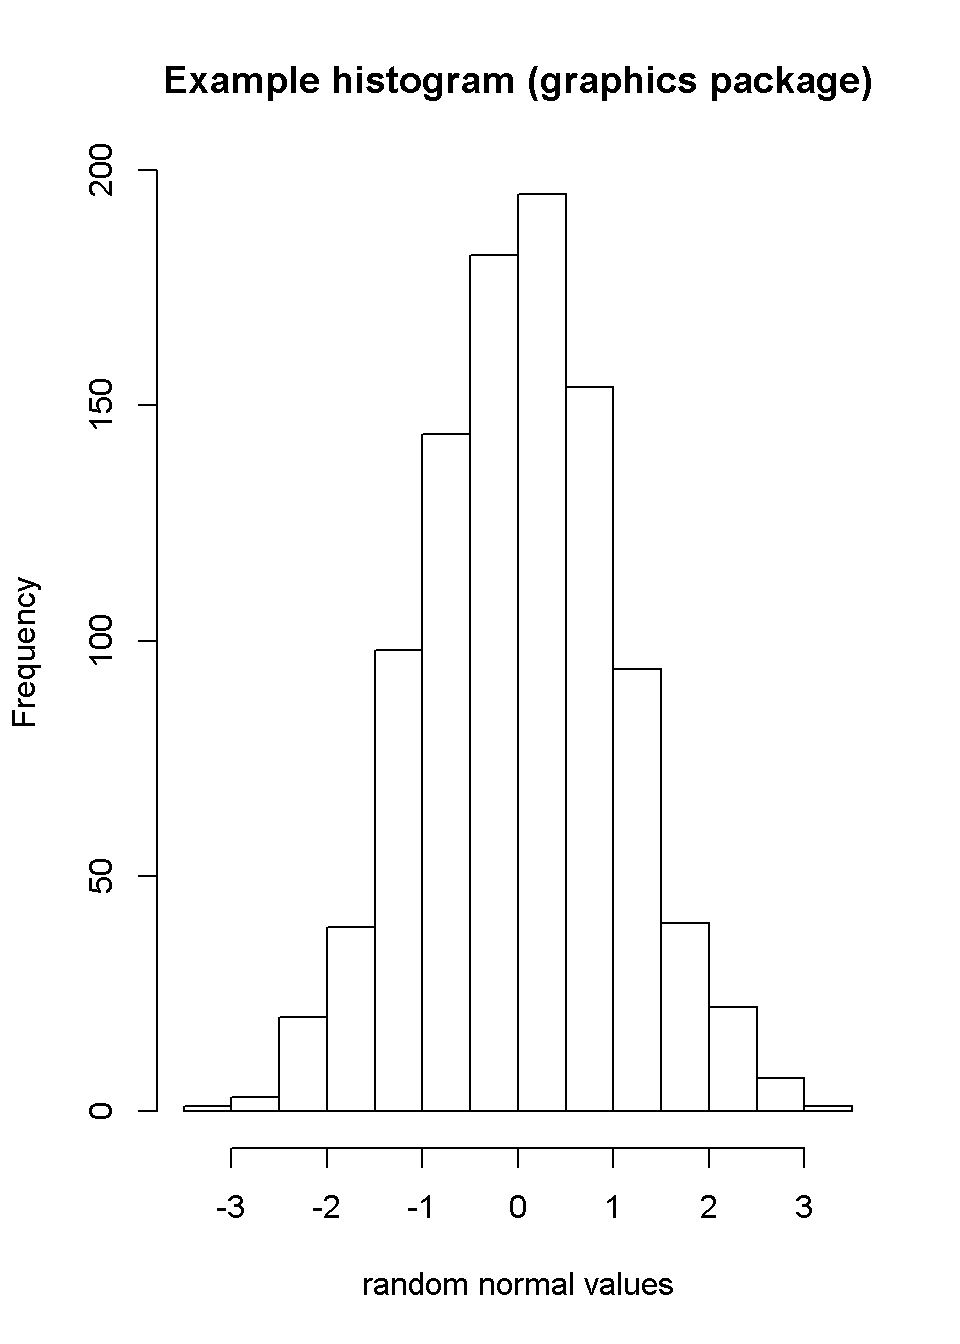
\includegraphics{04b-NewGraphCommands_files/figure-latex/exampleHist-1.pdf}
\caption{\label{fig:exampleHist-1}testing examples}
\end{figure}

\begin{verbatim}
> MyHist
$breaks
 [1] -3.5 -3.0 -2.5 -2.0 -1.5 -1.0 -0.5  0.0  0.5  1.0  1.5  2.0  2.5  3.0  3.5

$counts
 [1]   2   4  12  42  89 141 202 187 155  98  41  20   5   2

$density
 [1] 0.004 0.008 0.024 0.084 0.178 0.282 0.404 0.374 0.310 0.196 0.082 0.040
[13] 0.010 0.004

$mids
 [1] -3.25 -2.75 -2.25 -1.75 -1.25 -0.75 -0.25  0.25  0.75  1.25  1.75  2.25
[13]  2.75  3.25

$xname
[1] "x"

$equidist
[1] TRUE

attr(,"class")
[1] "histogram"

> MyHist = hist(x, xlab = "random normal values", main = "Example histogram (BrailleR package)")
\end{verbatim}

\begin{figure}
\centering
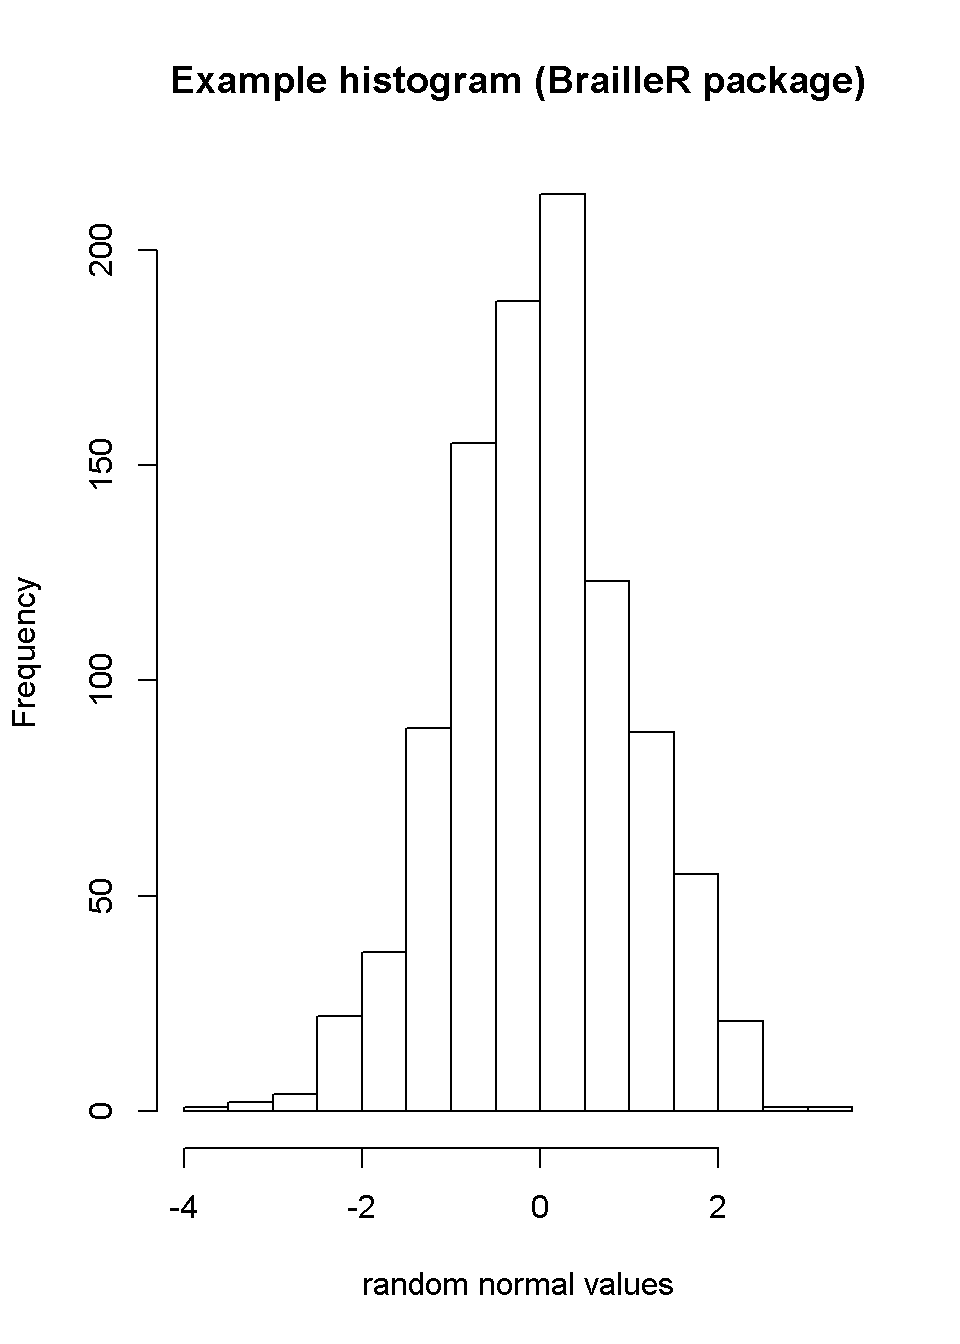
\includegraphics{04b-NewGraphCommands_files/figure-latex/exampleHist-2.pdf}
\caption{\label{fig:exampleHist-2}testing examples}
\end{figure}

\begin{verbatim}
> MyHist
$breaks
 [1] -3.5 -3.0 -2.5 -2.0 -1.5 -1.0 -0.5  0.0  0.5  1.0  1.5  2.0  2.5  3.0  3.5

$counts
 [1]   2   4  12  42  89 141 202 187 155  98  41  20   5   2

$density
 [1] 0.004 0.008 0.024 0.084 0.178 0.282 0.404 0.374 0.310 0.196 0.082 0.040
[13] 0.010 0.004

$mids
 [1] -3.25 -2.75 -2.25 -1.75 -1.25 -0.75 -0.25  0.25  0.75  1.25  1.75  2.25
[13]  2.75  3.25

$xname
[1] "x"

$equidist
[1] TRUE

$main
[1] "Example histogram (BrailleR package)"

$xlab
[1] "random normal values"

$ExtraArgs
$ExtraArgs$main
[1] "Histogram of x"

$ExtraArgs$xlab
[1] "x"

$ExtraArgs$ylab
[1] "Frequency"

$ExtraArgs$sub
[1] ""


$NBars
[1] 14

$par
$par$xaxp
[1] -3  3  6

$par$yaxp
[1]   0 200   4


$xTicks
[1] -3 -2 -1  0  1  2  3

$yTicks
[1]   0  50 100 150 200

attr(,"class")
[1] "Augmented" "histogram"

> VI(MyHist)
This is a histogram, with the title: Histogram of x
"x" is marked on the x-axis.
Tick marks for the x-axis are at: -3, -2, -1, 0, 1, 2, and 3 
There are a total of 1000 elements for this variable.
Tick marks for the y-axis are at: 0, 50, 100, 150, and 200 
It has 14 bins with equal widths, starting at -3.5 and ending at 3.5 .
The mids and counts for the bins are:
mid = -3.25  count = 2 
mid = -2.75  count = 4 
mid = -2.25  count = 12 
mid = -1.75  count = 42 
mid = -1.25  count = 89 
mid = -0.75  count = 141 
mid = -0.25  count = 202 
mid = 0.25  count = 187 
mid = 0.75  count = 155 
mid = 1.25  count = 98 
mid = 1.75  count = 41 
mid = 2.25  count = 20 
mid = 2.75  count = 5 
mid = 3.25  count = 2
\end{verbatim}

When you first issued the \texttt{library(BrailleR)} command, there were several warnings printed out. One of them told you that the \texttt{hist()} function from the \texttt{graphics} package was masked by the \texttt{BrailleR} version. This means that when you use \texttt{hist()}, it is the \texttt{BrailleR} version being used.

the \texttt{BrailleR} package includes \texttt{hist()} and \texttt{boxplot()} functions that pass the details of the command on to the \texttt{graphics} package functions of the same name, and then add any additional content required that will improve the ability to describe the visual graphic produced in text. In most cases, the graph producing functions pass on arguments such as \texttt{main}, \texttt{xlab}, or \texttt{ylab} (for main title and axis labels) to the relevant plotting commands without storing these elements in the object that is created. These elements are stored as graphical parameters and can be recalled using \texttt{par()} commands.

\hypertarget{scatter-plots}{%
\section{Scatter plots}\label{scatter-plots}}

The description of the \texttt{hist()} function given above shows what is possible if a graph is created using a specific function. Many types of graphs are created using the \texttt{plot()} function which is actually a family of functions tailored to the type of object pushed into them. In addition, the \texttt{plot()} command is used to generate a simple scatter plot. This is slightly unfortunate in a theoretical sense, but useful in a practical sense. The use of \texttt{plot()} to generate a scatter plot cannot lead to a graph that the \texttt{VI()} functionality can work with. Unlike the \texttt{hist()} command which can be replaced by a function of the same name in the \texttt{BrailleR} package, the solution needs to be a new function of a new name. In addition to the new \texttt{ScatterPlot()} function, the \texttt{BrailleR} package has a \texttt{FittedLinePlot()} function that adds a fitted line to the scatter plot.

The example given on the help page for \texttt{ScatterPlot()} proves that the plots generated by \texttt{ScatterPlot()} and \texttt{FittedLinePlot()} are identical to those that would normally be created using \texttt{plot()} and the addition of the fitted line using \texttt{abline()}. Running the command, \texttt{example(ScatterPlot)} command will give you the following:

\begin{verbatim}
> attach(airquality)

> op = par(mfcol = c(3, 2))

> plot(Wind, Ozone, pch = 4)
\end{verbatim}

\begin{verbatim}
> test1 = ScatterPlot(Wind, Ozone, pch = 4)
\end{verbatim}

\begin{verbatim}
> test1
\end{verbatim}

\begin{verbatim}
> plot(Wind, Ozone)
\end{verbatim}

\begin{verbatim}
> abline(coef(lm(Ozone ~ Wind)), col = 4)

> test2 = FittedLinePlot(Wind, Ozone, line.col = 4)
\end{verbatim}

\begin{verbatim}
> test2
\end{verbatim}

\begin{figure}
\centering
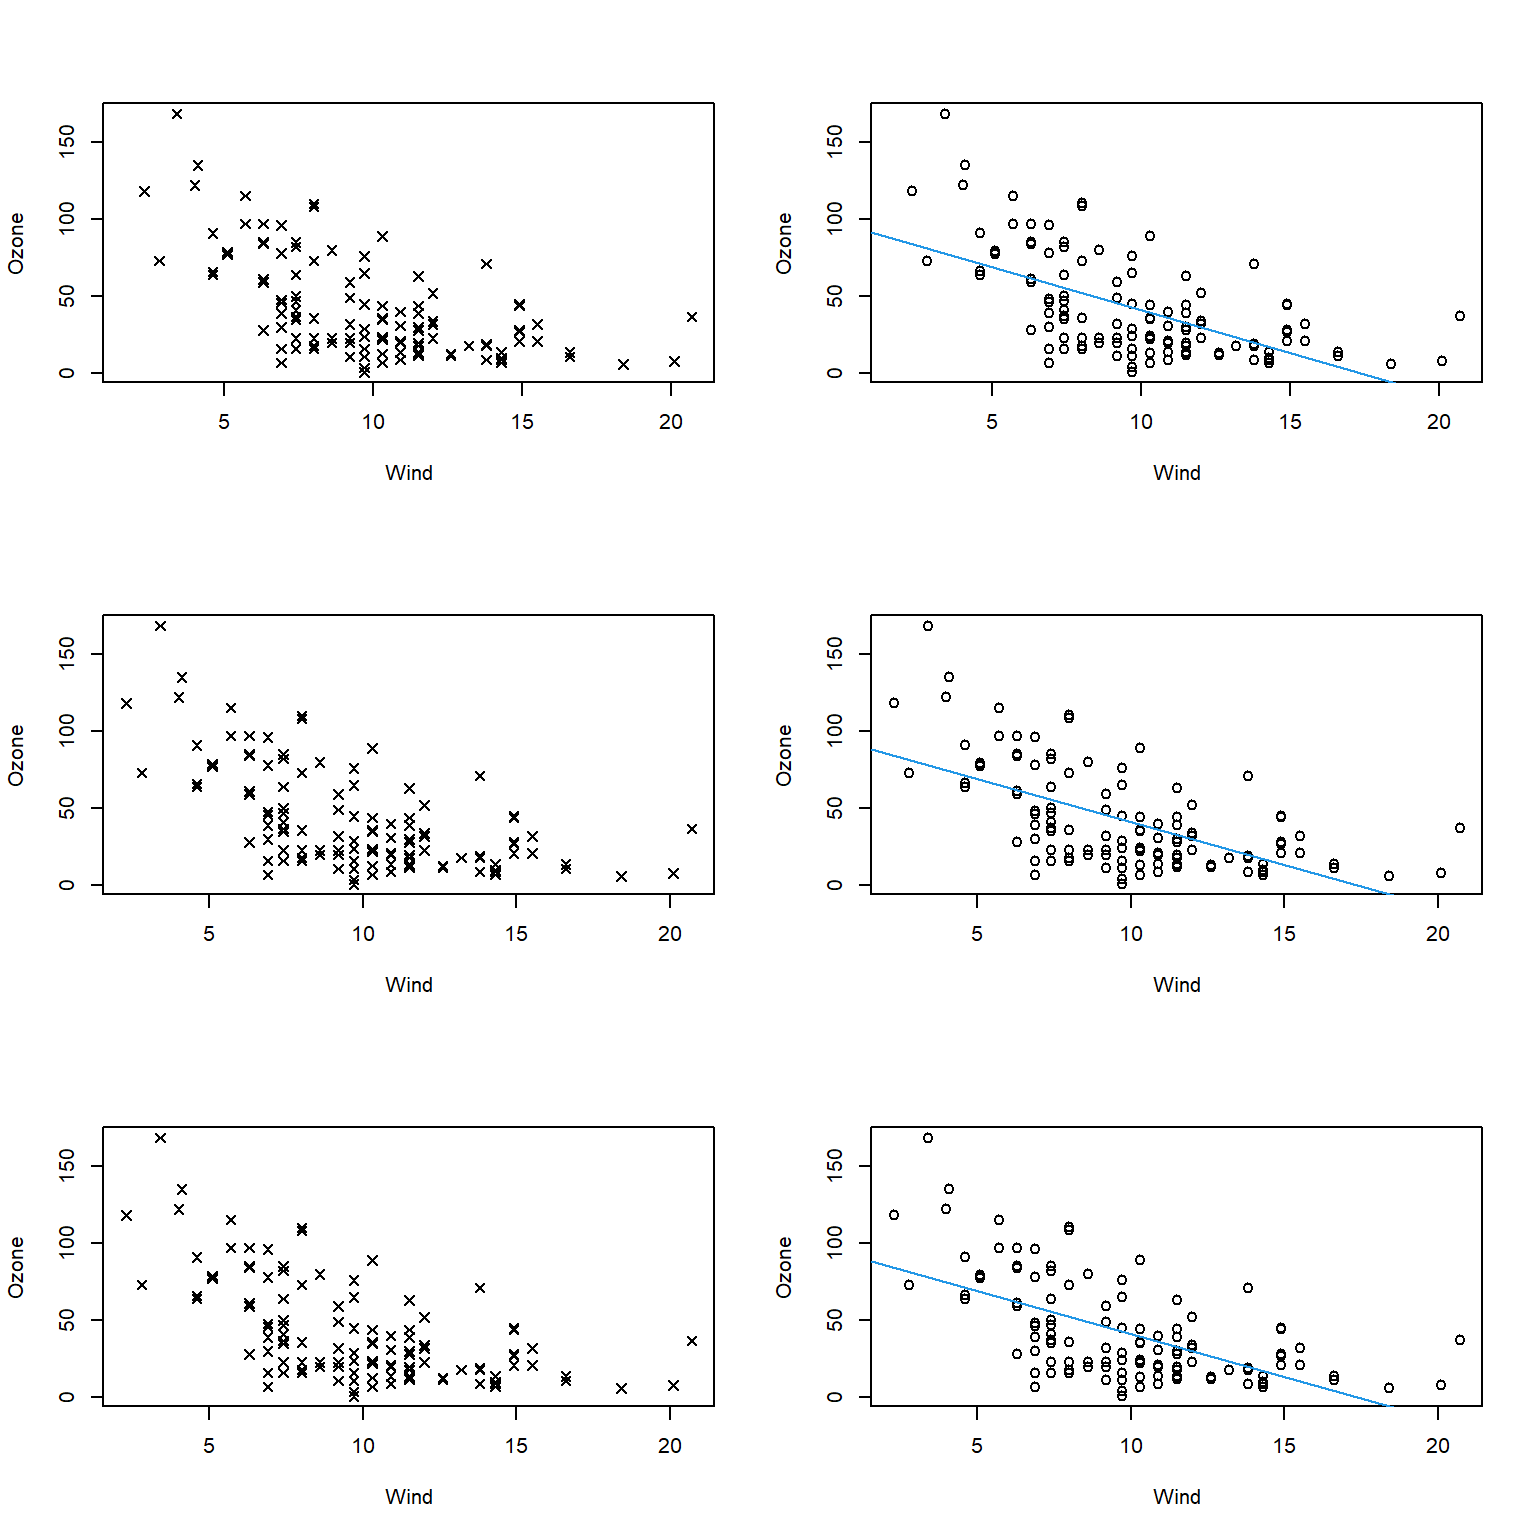
\includegraphics{04b-NewGraphCommands_files/figure-latex/exampleScatterPlot-1.pdf}
\caption{\label{fig:exampleScatterPlot}The six graphs generated by the \texttt{example(ScatterPlot)}}
\end{figure}

\begin{verbatim}
> par(op)

> detach(airquality)

> rm(test1)

> rm(test2)

> rm(op)
\end{verbatim}

\hypertarget{whats-in-the-scatter-plot}{%
\subsection{What's in the scatter plot?}\label{whats-in-the-scatter-plot}}

Well first we might ask what is in the graph window to be confident that a plot was actually made. The \texttt{WTF()} command was put in \texttt{BrailleR} to address this problem. For the record, WTF is the acronym for ``What's this figure?'' We'll see it's use in the next figure. It should tell us what appears in the graph window for things like axis lables and titles.

The current solution offered by the \texttt{BrailleR} package for helping describe the points plotted in a scatter plot, is to attempt to replicate the summarisation done by sight using a text construct. A sighted person looking at a scatter plot might look at the trend being displayed by a set of points, but they might as easily partition the plot area into a grid pattern and recognize the density of points in each region. For example,

\begin{Shaded}
\begin{Highlighting}[]
\FunctionTok{attach}\NormalTok{(airquality)}
\FunctionTok{plot}\NormalTok{(Wind, Ozone, }\AttributeTok{pch =} \DecValTok{4}\NormalTok{)}
\FunctionTok{abline}\NormalTok{(}\AttributeTok{v=}\FunctionTok{min}\NormalTok{(Wind)}\SpecialCharTok{+}\FunctionTok{c}\NormalTok{(}\FloatTok{0.25}\NormalTok{,}\FloatTok{0.5}\NormalTok{,}\FloatTok{0.75}\NormalTok{)}\SpecialCharTok{*}\NormalTok{(}\FunctionTok{max}\NormalTok{(Wind)}\SpecialCharTok{{-}}\FunctionTok{min}\NormalTok{(Wind)), }\AttributeTok{col=}\DecValTok{6}\NormalTok{)}
\FunctionTok{abline}\NormalTok{(}\AttributeTok{h =} \FunctionTok{min}\NormalTok{(Ozone, }\AttributeTok{na.rm=}\ConstantTok{TRUE}\NormalTok{) }\SpecialCharTok{+}\FunctionTok{c}\NormalTok{(}\FloatTok{0.25}\NormalTok{,}\FloatTok{0.5}\NormalTok{,}\FloatTok{0.75}\NormalTok{)}\SpecialCharTok{*}\NormalTok{(}\FunctionTok{max}\NormalTok{(Ozone, }\AttributeTok{na.rm=}\ConstantTok{TRUE}\NormalTok{)}\SpecialCharTok{{-}}\FunctionTok{min}\NormalTok{(Ozone, }\AttributeTok{na.rm=}\ConstantTok{TRUE}\NormalTok{)), }\AttributeTok{col=}\DecValTok{6}\NormalTok{)}
\FunctionTok{WTF}\NormalTok{()}
\end{Highlighting}
\end{Shaded}

\begin{figure}
\centering
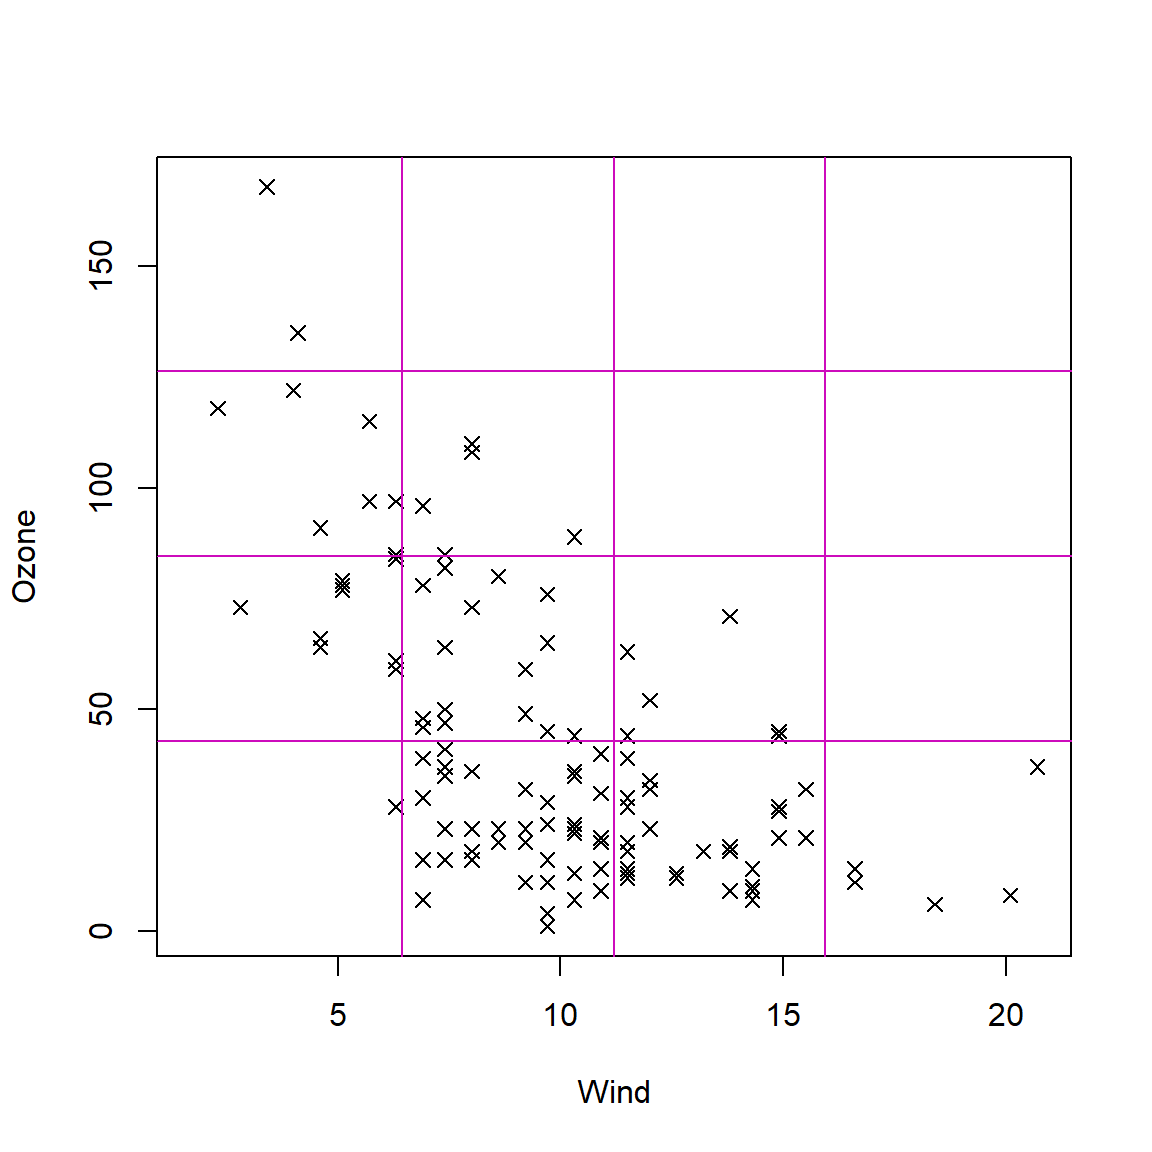
\includegraphics{04b-NewGraphCommands_files/figure-latex/addGridLines-1.pdf}
\caption{\label{fig:addGridLines}Scatter plot of Ozone versus Wind with grid lines added.}
\end{figure}

\begin{verbatim}
This graph has no main title;  and o subtitle;
"Wind" as the x axis label;
"Ozone" as the y axis label;
There are 116 points marked on this graph.
\end{verbatim}

\begin{Shaded}
\begin{Highlighting}[]
\FunctionTok{detach}\NormalTok{(airquality)}
\end{Highlighting}
\end{Shaded}

Counting the number of points falling into each cell of the graphic and presenting the results as a table would give the reader an impression of the density of those points. The grid lines added in this last figure were spaced uniformly, and chosen to split the region into a \(4\times4\) grid of sixteen cells.
Refining the number of cells and the distributional assumptions for the grid lines should make it easier to understand the relationship between the two variables being plotted. Note that the general picture is what is sought, not the specific locations of every point. The number of points for the last scatter plot are counted by the \texttt{WhereXY()} command as follows:

\begin{Shaded}
\begin{Highlighting}[]
\FunctionTok{attach}\NormalTok{(airquality)}
\FunctionTok{WhereXY}\NormalTok{(Wind, Ozone, }\AttributeTok{grid =} \FunctionTok{c}\NormalTok{(}\DecValTok{4}\NormalTok{,}\DecValTok{4}\NormalTok{))}
\end{Highlighting}
\end{Shaded}

\begin{verbatim}
     1  2  3 4 Sum
4    2  0  0 0   2
3    7  5  0 0  12
2    9 15  6 0  30
1    1 39 27 5  72
Sum 19 59 33 5 116
\end{verbatim}

\begin{Shaded}
\begin{Highlighting}[]
\FunctionTok{detach}\NormalTok{(airquality)}
\end{Highlighting}
\end{Shaded}

In situations where the user is confident that the marginal distributions of either or both of the variables being plotted are normal, the grid lines should be spaced accordingly.

\hypertarget{brailler-commands-used-in-this-chapter-2}{%
\section{BrailleR commands used in this chapter}\label{brailler-commands-used-in-this-chapter-2}}

The BrailleR versions of the \texttt{hist()} and \texttt{boxplot()} commands replace those found in the \texttt{graphics} package. The BrailleR commands \texttt{ScatterPlot()} and \texttt{FittedLinePlot()} are specific to BrailleR and replace the functionality usually obtained through use of \texttt{plot()} and \texttt{abline()}. The \texttt{WTF()} command helped prove a graph has appeared in the graph window, and \texttt{WhereXY()} has helped count the number of points falling into subregions of the plotting area.

\hypertarget{WorkingBlind}{%
\chapter{Ways of Working in R as a Blind User}\label{WorkingBlind}}

This chapter presents some strategies to offer blind users options for producing and saving work from an R session. They complement the workflows used by sighted people, or replace the tools used by sighted people that are not able to be used by a blind person.

\hypertarget{a-little-background}{%
\section{A little background}\label{a-little-background}}

A major issue for blind users of any mathematical or statistical software is how the work that has been done will be transferred into a form that can be included in reports or assignments.
Standard methods of working with R are possible as a blind user, but there is one crucial task that sighted users find very easy that is beyond the reach of the blind user.
A sighted user can highlight a section of the output window (including commands and results) and copy the text into a document using the mouse. This task is done easily in word processing or text documents using keyboard commands by the blind user, but is often impractical or impossible within many software applications. A solution has been provided within the \texttt{BrailleR} package by adapting a tool developed by another R user for a completely different purpose. The \texttt{TeachingDemos} package \citep{Rpkg-TeachingDemos}, provided this tool. The original purpose was to quickly retain the output from an R session for distribution to students, and later in its
development, to create output files (in MS Word or HTML) that would log the progress through an assignment question or project.

\hypertarget{using-plain-text-files}{%
\section{Using plain text files}\label{using-plain-text-files}}

The code for saving the basic text output and commands being generated during an interactive session into a plain text file was among the early developments of the \texttt{BrailleR} package.
The functions \texttt{txtStart()}, \texttt{txtStop()}, \texttt{txtComment()}, and \texttt{txtSkip()} were copied (with permission) from the \texttt{TeachingDemos} package; in addition, a \texttt{txtOut()} function that simplifies use of \texttt{txtStart()} was added to the \texttt{BrailleR} package.

\hypertarget{use-of-r-markdown}{%
\section{Use of R markdown}\label{use-of-r-markdown}}

The general uptake of reproducible research ideas by many in the R community has vastly improved the opportunities for novice R users to create well-formatted HTML documents from markdown documents.
This change in the general mindset has huge benefits for a blind user.
An R markdown file is just plain text and is therefore accessible.
Even more impressive, is that the HTML documents that result from these files are also very accessible to a blind reader. I discovered the potential for R markdown to make life so much easier for blind students by attending a workshop delivered by Yihui Xie at the 2014 UseR conference in Los Angeles. His book \citep{Xie2015} serves as the guide by which I create a lot of R markdown content including this book.

The greatest challenge for blind R users who want to get into R markdown is that the majority of resources on the subject assume use of RStudio \citep{RStudio} which is not accessible to a screen reader user. Use of RStudio is not essential. For example, a basic R markdown document might start like the following:

\begin{verbatim}
---
title: ""
author: ""
date: ""
output:
    html_document:
        toc: false
        number_sections: false
        fig_height: 7
        fig_width: 7
--- 

 ```{r ChunkName}
...
```
\end{verbatim}

This text needs to be saved in a text file, usually with the file extension ``Rmd''. It has two parts. The top section, starting and finishing with , is a YAML header and establishes settings for the document. You will need to fill in the gaps between double quotes for the document's title, your name, and the date, but otherwise you can leave this section alone for the time-being.

The second section is an empty R chunk. The opening line starts with three accent grave symbols (sometimes called backticks) and then some details used only for this chunk. The details in this chunk header say to process the upcoming commands using R and that the chunk currently has the label ``ChunkName'' which you would normally change to something more meaningful. The second line of this section is where you would put an R command (instead of the meaningless dots put there now), and the last line is how we close a chunk (using those backticks again). You can put a whole series of R commands in the middle, but the chunk must start and finish with \texttt{\textasciigrave{}\textasciigrave{}\textasciigrave{}} if the document is to be processed properly.

To get this R markdown content to be converted to HTML, you must complete the following steps:

\begin{enumerate}
\def\labelenumi{\arabic{enumi}.}
\tightlist
\item
  Save the above content into a text file and name it ``FirstGo.Rmd''. N.B. This must be plain text.
\item
  Edit the bits I suggested above. In fact, the bare minimum is to put a valid R command in the middle of the R chunk.
\item
  Put this file in the current working directory. Check what this is using \texttt{getwd()} if you need to be sure.
\item
  Type the command \texttt{rmarkdown::render("FirstGo.Rmd")}
\end{enumerate}

You should see that this command generates a little output in the R session window and that a file called ``FirstGo.html'' has been created. Open that file now.

The basic steps followed by all users of R markdown files are:

\begin{enumerate}
\def\labelenumi{\arabic{enumi}.}
\tightlist
\item
  Update the Rmd file.
\item
  ``Knit'' the R markdown file; The word ``knit'' comes from the R package that does the work here.
\item
  Review the impact on your HTML file. You might need to refresh the browser if the file is still open.
\end{enumerate}

You can:

\begin{itemize}
\tightlist
\item
  add more R chunks; give them distinct labels though.
\item
  Write plain text in between chunks;
\item
  Add section headings; use number signs \texttt{\#} at the start of a line that you want to be a heading. The level of heading is determined by the number of number signs you use.
\item
  Add mathematical expressions using standard LaTeX notation; single or double dollar signs denote the start and end of mathematical content.
\item
  \ldots{} and so much more.
\end{itemize}

Remember: This book is written entirely in R markdown. If you see something here, then you can have it in your own R markdown work!

We will see the power of R markdown for doing some tasks using the \texttt{BrailleR} package in Chapter \ref{RMarkdown} and start using WriteR as a substitute for RStudio in Chapter \ref{WriteR}.

\hypertarget{running-jobs-offline}{%
\section{Running jobs offline}\label{running-jobs-offline}}

Blind users will benefit from switching to batch processing commands using \texttt{R\ CMD\ BATCH} at the command line, using the reproducible research functionality offered by the \texttt{knitr} package, or both strategies. Functions to help users (working under Windows operating systems) move to these ways of working have been included in the \texttt{BrailleR} package. In particular, a Windows user can use the \texttt{MakeBatch()} function to create a batch file in the current working directory, which creates the single command line that would be called to process a specified R script or R markdown file appropriately. The \texttt{BrailleR} package also shows a user how a test file would be processed using these batch files. Conversion of an R script or the history of the current workspace to an R markdown file are implemented using the \texttt{R2Rmd()} and \texttt{History2Rmd()} functions respectively. This suite of functions should assist the blind user migrate to the more efficient methods of working and ultimately become more proficient and efficient than their peers who are not yet making use of the reproducible research type of workflow.

\hypertarget{RMarkdown}{%
\chapter{Use of R markdown to generate an analysis efficiently}\label{RMarkdown}}

In a general sense, R markdown has been used to create reports and package vignettes because it creates an analysis that is reproducible. The \texttt{BrailleR} package started to use R markdown in late 2014 as a method for generating simple analyses that might be needed by students taking introductory statistics courses. Since that time, the prevalence of R markdown as a teaching tool in these courses has increased. The functions described below are therefore also generating example R markdown files to help learn how to use R markdown. The workflow illustrated in this chapter is also the workflow used to create this book. It is heavily reliant on the work of Yihui Xie, much of which can be found in \citep{Xie2015}.

You will need the \texttt{BrailleR} package to be ready for use to follow along with the examples in this chapter. Do this by issuing the command \texttt{library(BrailleR)} now.

\hypertarget{general-information}{%
\section{General information}\label{general-information}}

Each command described in this chapter and other similar commands draft a new R markdown file and then compile it to an HTML file that is easily read by a screen reader user. They make extensive use of the \texttt{knitr} package \citep{Rpkg-knitr} to process R commands and retrieve the R output and graphs, and then the \texttt{rmarkdown} package \citep{Rpkg-rmarkdown} to process the markdown content of the raw input file into HTML (or other file types if we wanted them).

This HTML file is opened automatically if R is being used interactively, giving the blind user immediate access to the information. The content is automatically presented using sufficiently marked up HTML code including headings and tables so that the blind user can make best use of their screen reading software. All graphs are given an ``alt tag'' when they are included in the HTML file, and can be presented using a text description available from the \texttt{VI()} functionality of the \texttt{BrailleR} package.

In addition, the blind user may need one or more of the graphs in a variety of formats (png, pdf, eps, or svg), nicely formatted tables for insertion into documents (LaTeX or HTML), and access to the code that generated these graphs and tables (an R script).
This is handled using add-on packages wherever possible so that blind users are completing tasks using the same tools as their sighted peers. For example, nicely tabulated results can be saved as individual text files for later inclusion in LaTeX documents using the \texttt{xtable} package \citep{Rpkg-xtable}.

The commands shown in this chapter make use of R markdown, but they are not actually ready for direct use within other R markdown documents.
If you wish to get the output you observe within the HTML documents that will be generated, you will need to extract the relevant parts of the R markdown script files that the commands create. That sounds harder than it is!

\hypertarget{replacing-the-graphic-user-interface-gui}{%
\section{Replacing the Graphic User Interface (GUI)}\label{replacing-the-graphic-user-interface-gui}}

One major criticism of R often heard from novice users is that a graphic user interface (GUI) is much easier to use than the command line mode of operation. Blind users are no different in this respect, but as has been reported previously \citep{GodfreyRJournal}, none of the GUI-based front ends for R are accessible to the blind user.
When considering the benefits of using a GUI mode of operation, we turn to the justification used for the creation of some of these interfaces; redacting all references to the GUI helps emphasize the reasons for their existence:

\begin{itemize}
\tightlist
\item
  R Commander aims ``to support \ldots{} the statistical functionality required for a basic-statistics course; to make it relatively difficult to do unreasonable things;
  and to render visible the relationship between choices made \ldots{}\\
  and the R commands that they generate.'' \citep{Fox2005-RCommander}.
\item
  ``Because R analyses must be called as text commands, the user is required to find out the name of the function that will accomplish their task, and then remember that name along with the names of the variables to feed it, and its argument options. Perhaps more fundamentally, many users have never dealt with a program that requires them to type in commands that manipulate objects in the program.
  For beginners, Deducer is designed to be an intuitive dialog based interface to common data manipulation and analysis tasks.'' \citep{Fellows2012Deducer}
\item
  ``The scope of RKWard is deliberately broad, targeting both R novices and experts. For the first group, the aim is to allow any person with knowledge on statistical procedures to start using RKWard for their everyday work without having to learn anything about the R programming language, at least initially. At the same time, RKWard tries to support users who want to learn and exploit the full flexibility of the R language for automating or customizing an analysis.'' \citep{RoedigerEtAl2012RKWard}
\item
  RKWard ``avoids wrapping complex sequences of data manipulation or analysis into custom highlevel R functions. The task of providing high-level functions is logically independent of the development of the GUI frontend, and should best be addressed in dedicated R packages, where
  necessary.'' \citep{RoedigerEtAl2012RKWard}
\end{itemize}

Making any of these GUI tools accessible is
difficult because they were not developed using interface development toolkits that automatically build accessibility into the interface.
Creation of a GUI such as R Commander is not a small undertaking. Retrospectively building in the necessary accessibility features would be a massive undertaking that the blind community could not reasonably expect of a very small development team. Duplicating the work done to create such a GUI tool from scratch using a development toolkit that helps build in the necessary elements for accessibility and then maintaining it as operating systems develop over time is not a practical solution either. It may be possible to improve the toolkits that are used to create the GUI options like R Commander or Deducer so that their development is not hindered while their accessibility becomes automatic; unfortunately, this requires knowledge well beyond my skill set.

If blind users cannot make use of any of the GUI tools and we don't have the necessary skills to develop such a tool that does work for ourselves, what solutions exist for us? When I've discussed the merits of various statistical software with other blind users, they have questioned the use of R by saying something like, ``When I use software \emph{x}, I can do \emph{y} and \emph{z}. How do I do that in R?'' With respect to SAS for example, a user can build up a set of templates for various commonly used analyses for themselves. The same is true as an R user, but SAS users can get the templates by using the menus in the standard GUI, and they can keep the procedures in files for later use. SPSS users can do this as well. (These seem to be the most commonly used software options for blind users who communicate with me.) In either case, the code can be reused after issuing a few find/replace searches. It seems that even though it is more efficient to make use of this ability to re-use code templates, that many of the blind users of these software options prefer to use key presses to simulate mouse clicks in order to use the menus and dialogue boxes. When questioning them on their motives, we quickly come to the point that the use of menus and dialogue boxes offers a degree of comfort that tasks have been done correctly. The next crucial aspect worth mentioning is that the GUI provides the user with more output than can be obtained from typing out numerous commands in R. Searching for the right functions and then ensuring the syntax of their arguments is correct limits a blind user's ability in any command-line software, just as it does for sighted users.

The solution for a replacement of the GUI is to create convenience functions with simple names that require entry of a minimal number of arguments so that the user gets the maximum amount of useful information. This information might prove more than is needed for many users, but hopes to deliver what is needed by the widest possible range of blind users.
Like RKWard, \texttt{BrailleR} functions generate R scripts that are somewhat verbose \citep{RoedigerEtAl2012RKWard}.

\hypertarget{description-of-a-single-numeric-variable}{%
\section{Description of a single numeric variable}\label{description-of-a-single-numeric-variable}}

There are many commands needed to get the numeric and graphic summary measures that might be required to collect all relevant information on a single numeric variable. The \texttt{UniDesc()} command has been written as a shortcut for a blind user who wishes to obtain:

\begin{itemize}
\tightlist
\item
  the counts of points in the sample that were observed and not observed,
\item
  the mean and trimmed mean,
\item
  the five number summary: minimum, lower quartile, median, upper quartile, and maximum,
\item
  the interquartile range (IQR) and standard deviation,
\item
  measures of skewness and kurtosis, relying on the \texttt{moments} package \citep{Rpkg-moments},
\item
  a histogram and/or a boxplot,
\item
  a normality (quantile-quantile) plot,
\item
  various tests for normality, courtesy of the \texttt{nortest} package \citep{Rpkg-nortest} , and
\item
  tests on the significance of the skewness and kurtosis, also courtesy of the \texttt{moments} package \citep{Rpkg-moments}.
\end{itemize}

The \texttt{UniDesc()} function can deliver all of this with minimal effort from the user.

An example of the main output document (HTML) can be viewed by re-issuing the commands generated by calling

\begin{Shaded}
\begin{Highlighting}[]
\FunctionTok{example}\NormalTok{(UniDesc)}
\end{Highlighting}
\end{Shaded}

while running R interactively. This issues the following commands.

\begin{verbatim}
DIR = getwd()
setwd(tempdir())
Ozone=airquality$Ozone
UniDesc(Ozone)
rm(Ozone)
# N.B. Various files and a folder were created in a temporary directory. 
# Please investigate them to see how this function worked.
setwd(DIR)
\end{verbatim}

As an alternative, and if you do have a current internet connection you can view the result of running the \href{https://R-Resources.massey.ac.nz/BrailleRInAction/Ozone-UniDesc.html}{\texttt{UniDesc()} command on the Ozone data} in your browser without having to re-enter the example commands. You can also view the \href{Ozone-UniDesc.Rmd}{R markdown script created by \texttt{UniDesc(Ozone)}} which starts with the following lines:

\begin{verbatim}
# Univariate analysis for Ozone 
#### Prepared by Jonathan Godfrey   

```{r setup, purl=FALSE, include=FALSE}
library(BrailleR)
opts_chunk$set(dev=c("png", "pdf", "postscript", "svg"))
opts_chunk$set(comment="", echo=FALSE, fig.path="Ozone/Ozone-", fig.width=7)
```  

## Basic summary measures

```{r BasicSummaries}
Ozone.count = length(Ozone)
Ozone.unique = length(unique(Ozone))
Ozone.Nobs = sum(!is.na(Ozone))
Ozone.Nmiss = sum(is.na(Ozone))
Ozone.mean = mean(Ozone, na.rm = TRUE)
Ozone.tmean5 = mean(Ozone, trim =0.025, na.rm = TRUE)
Ozone.tmean10 = mean(Ozone, trim =0.05, na.rm = TRUE)
Ozone.IQR = IQR(Ozone, na.rm = TRUE)
Ozone.sd = sd(Ozone, na.rm = TRUE)
Ozone.var = var(Ozone, na.rm = TRUE)
Ozone.skew = moments::skewness(Ozone, na.rm = TRUE)
Ozone.kurt = moments::kurtosis(Ozone, na.rm = TRUE)
``` 
... ... ...
\end{verbatim}

The full R markdown file can be opened in any text editor. A Windows user can open the file created by the \texttt{example(UniDesc)} command above, by issuing the command \texttt{Notepad("Ozone-UniDesc.Rmd")} at the R prompt. Opening the Windows Explorer file browser will help you select an alternative text editor; you can do this by typing \texttt{Explorer()}.

The document header includes a code chunk that sets the options for the \texttt{knit2html()} process used to convert this file to HTML.
This processing allows for:

\begin{itemize}
\tightlist
\item
  multiple file types for the graphs,
\item
  ensures a minimum of extra text in the output,
\item
  hides the R code from the HTML file,
\item
  sets the location of the saved graphs, and
\item
  establishes the height of the figures.
\end{itemize}

The user that does not like these settings can edit the markdown file for themselves and re-process the file, but the intention is to deliver more than all users would want so that as many users as possible get what they need.

This R markdown script uses the \texttt{VI()} method for the graphs as well as the code that generates the HTML (via markdown) and LaTeX tables (using the \texttt{xtable} package). Take note of the arguments supplied to the code chunks for the graphs; these include a \texttt{fig.cap} which is used as an Alt tag in the resulting HTML files. The quoted string is the only text that is read aloud by a blind person's screen reading software as they move the cursor onto the graph while reading through the HTML document. The methods used for creating tables in markdown (either directly or using the \texttt{kable()} command from the \texttt{knitr} package) \citep{Rpkg-knitr} both lead to a formatted HTML table that is easily navigated by a screen reader using keystrokes that help move between rows or columns. The result is that the HTML document is about as user-friendly as can be expected for a blind user. It is important to recognize that some of the text is arranged for the optimal use by a blind person; it is possible to alter the cosmetics of the HTML document without altering the experience for blind users. Given a blind user might be accompanied by sighted classmates, teaching staff, or colleagues, making the HTML pages presentable is desirable; this has been achieved using a custom style sheet (CSS) included in the package. This style includes some color, adequate spacing of content and other features that improve the clarity of the presented material which is important for a user with some residual vision that wishes to read through the results visually rather than using screen reading software.

If all of the optional arguments of the \texttt{UniDesc()} function are set at their defaults, the HTML file is automatically opened in a browser (courtesy of the \texttt{View} argument); it puts the R markdown file, the R script, and the HTML document in the current working directory, while the LaTeX and graph files are all placed in a subdirectory.

Several other convenience functions have been created that follow the same process as the \texttt{UniDesc()} function. The \texttt{OneFactor()} function compares one continuous response variable to a categorical variable, while \texttt{TwoFactors()} allows for two categorical variables and their possible interaction to help explain a single continuous response variable. These functions create group summary statistics and suitable graphs that a sighted audience might expect to see. Comparing a continuous response variable to a continuous predictor variable is achieved using the \texttt{OnePredictor()} function. Each of these functions has an example using data from the \texttt{datasets} package \citep{Rpkg-base} so a user can see what can be expected from these functions.

\hypertarget{analysis-of-a-single-continuous-variable-with-respect-to-a-single-grouping-factor}{%
\section{Analysis of a single continuous variable with respect to a single grouping factor}\label{analysis-of-a-single-continuous-variable-with-respect-to-a-single-grouping-factor}}

There are many commands needed to get the numeric and graphic summary measures that might be required to collect all relevant information on a single numeric variable when it might depend on a grouping factor. The \texttt{OneFactor()} command has been written as a shortcut for a blind user who wishes to obtain:

\begin{itemize}
\tightlist
\item
  the counts of observations within each group,
\item
  the mean, standard deviation and standard error for each group,
\item
  comparative boxplots and/or dotplots,
\item
  the one-way analysis of variance, and
\item
  Tukey's Honestly Significant Difference (HSD) test on the significance of the between group differences.
\end{itemize}

There will be circumstances when the last, and perhaps evern second to last elements of this functionality are not justified by the outcome of issuing the earlier commands. In particular, generating the output from Tukey's HSD would not normally be sought unless the analysis of variance showed there was a significant difference between the group means. The choice of reading the output and subsequently using it are left to the user. In this respect, \texttt{BrailleR} has not become an expert system that decides to or not to provide something; the user is still expected to do the thinking about the relevance of each element of hte overall set of output provided.

An example of the main output document (HTML) can be viewed by re-issuing the commands generated by calling

\begin{Shaded}
\begin{Highlighting}[]
\FunctionTok{example}\NormalTok{(OneFactor)}
\end{Highlighting}
\end{Shaded}

while running R interactively. This issues the following commands.

\begin{verbatim}
DIR = getwd()
setwd(tempdir())
data(airquality)

# the following line  returns an error:
## OneFactor("Ozone", "Month", airquality, Folder=tempdir(), View=FALSE)
# so we make a copy of the data.frame, and fix that:

airquality2 = airquality
airquality2$Month = as.factor(airquality$Month)
# and now all is good to try:
OneFactor("Ozone", "Month", airquality2)
# N.B. Various files and a folder were created in a temporary directory. 
# Please investigate them to see how this function worked.
setwd(DIR)
\end{verbatim}

As an alternative, and if you do have a current internet connection you can view the result of running the \href{https://R-Resources.massey.ac.nz/BrailleRInAction/Ozone.Month-OneFactor.html}{\texttt{OneFactor()} command on the Ozone data} in your browser without having to re-enter the example commands.

The example here demonstrates the point that the grouping variable must be a factor. The month variable is not stored as a factor in the airquality data so its use would have created an error.

All elements of the analysis which incorporate graphical information, or text that is slow to read using a screen reader are processed using the \texttt{VI()} functionality.

\hypertarget{use-of-brailler-for-linear-regression}{%
\section{Use of BrailleR for linear regression}\label{use-of-brailler-for-linear-regression}}

Linear regression is almost always taught using graphical techniques, especially for the validation of the model being fitted. Of particular note is the way an instructor would teach sighted students about the sensibility of fitting any line to some data which cannot be easily judged even using the \texttt{WhereXY()} function described earlier. A blind student lacking an embosser to produce a tactile image that shows the fitted line and the data, will almost certainly need to fit the model and see how good or bad it is. These blind students are therefore even more reliant on the residual analysis than their sighted classmates

The \texttt{VI()} command can be applied to a linear model object. The specific function to do this is found in the \texttt{VI.lm()} function, but most users do not need to explicitly use \texttt{VI.lm()} because the call to \texttt{VI()} will know to use the \texttt{VI.lm()} function if it is the right one to use at the time.

The \texttt{VI.lm()} function generates so much text as a substitute for the graphs used by sighted users, that it is easier to put this text in an HTML document and have that new document opened in a browser instead of trying to use a screen reader within the R session.

Let's see an example using the \texttt{airquality} data.
Please note: The example is chosen for reproducibility and its lack of statistical validity, as this is the best way to demonstrate the function's value to a blind user.

A simple linear regression model might be created and investigated using:

\begin{Shaded}
\begin{Highlighting}[]
\FunctionTok{data}\NormalTok{(airquality)}
\NormalTok{MyModel }\OtherTok{=} \FunctionTok{lm}\NormalTok{(Ozone}\SpecialCharTok{\textasciitilde{}}\NormalTok{Wind, }\AttributeTok{data=}\NormalTok{airquality)}
\FunctionTok{summary}\NormalTok{(MyModel)}
\end{Highlighting}
\end{Shaded}

\begin{verbatim}
Call:
lm(formula = Ozone ~ Wind, data = airquality)

Residuals:
    Min      1Q  Median      3Q     Max 
-51.572 -18.854  -4.868  15.234  90.000 

Coefficients:
            Estimate Std. Error t value Pr(>|t|)    
(Intercept)  96.8729     7.2387   13.38  < 2e-16 ***
Wind         -5.5509     0.6904   -8.04 9.27e-13 ***
---
Signif. codes:  0 '***' 0.001 '**' 0.01 '*' 0.05 '.' 0.1 ' ' 1

Residual standard error: 26.47 on 114 degrees of freedom
  (37 observations deleted due to missingness)
Multiple R-squared:  0.3619,    Adjusted R-squared:  0.3563 
F-statistic: 64.64 on 1 and 114 DF,  p-value: 9.272e-13
\end{verbatim}

\begin{Shaded}
\begin{Highlighting}[]
\FunctionTok{par}\NormalTok{(}\AttributeTok{mfrow=}\FunctionTok{c}\NormalTok{(}\DecValTok{2}\NormalTok{,}\DecValTok{2}\NormalTok{))}
\FunctionTok{plot}\NormalTok{(MyModel)}
\end{Highlighting}
\end{Shaded}

\begin{figure}
\centering
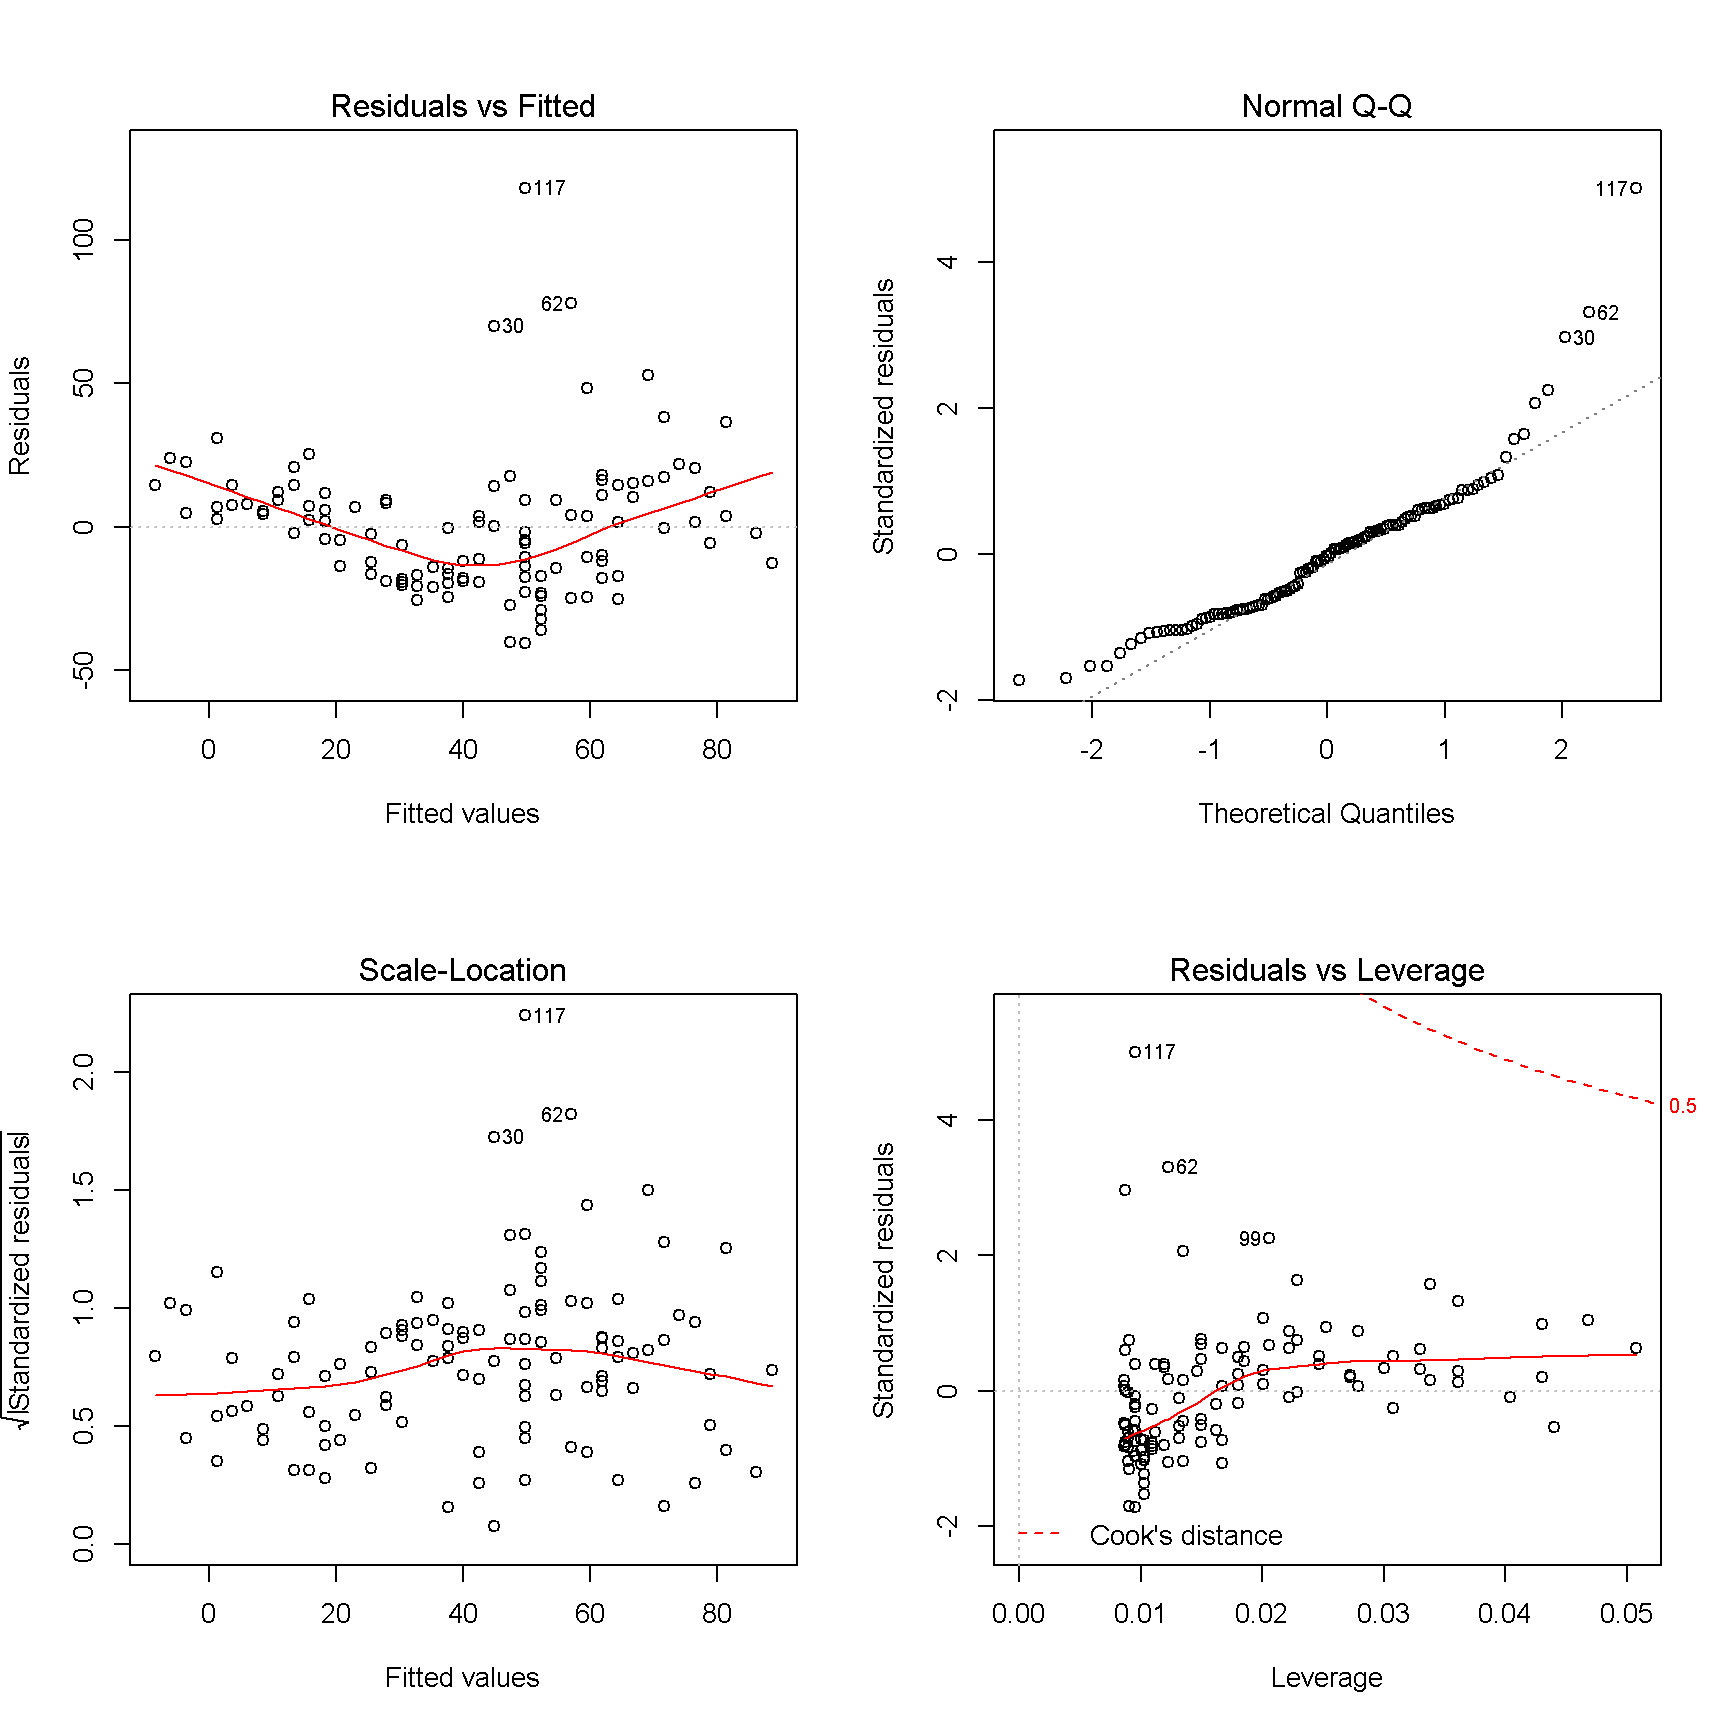
\includegraphics{05-MarkdownInAction_files/figure-latex/AirQuality.lm-1.pdf}
\caption{(\#fig:AirQuality.lm)Diagnostic plots for the simple linear regression model.}
\end{figure}

The user now has a model stored as \texttt{MyModel} in the current workspace, has printed a summary of that model, and has plotted a set of four diagnostic plots in a \(2\times{}2\) grid. The blind user will still need to issue those commands so that the output is created to meet the expectations of the sighted audience, but will also find value in issuing the two extra commands

\begin{Shaded}
\begin{Highlighting}[]
\FunctionTok{VI}\NormalTok{(MyModel)}
\FunctionTok{VI}\NormalTok{(}\FunctionTok{summary}\NormalTok{(MyModel))}
\end{Highlighting}
\end{Shaded}

The use of the second of these commands will generate

\begin{verbatim}
The term which is significant to 1% is
Wind with an estimate of -5.550923 and P-Value of 9.271974e-13 
\end{verbatim}

which will be a much easier reading exercise for a screen reader user than would be the standard \texttt{summary()} output given earlier. Note that not all the information contained in the standard summary is contained in this output.

The output from use of the \texttt{VI()} command on the linear model can be viewed in your browser if you have a current internet connection. If you do not have a connection at this time, you will need to re-issue some of the above commands for yourself in an R session.

The HTML document created by \texttt{VI.lm()} is based on the results of the \texttt{UniDesc()} function applied to the Pearson residuals for the model and a number of other graphs and tables used to validate the model. The included graphs are of the residuals plotted against the fitted values, the order the data were collected (assumes data are presented in this order), the leverages, and the preceding residual.
Each of these graphs is subjected to scrutiny using the \texttt{WhereXY()} function as described earlier. The marginal distribution of the residuals is assumed normal while the fitted values and leverages are categorized on the basis of a uniform distribution. The assumption of normality for residuals is immediately obvious, but the choice to explicitly use an incorrect assumption of uniformity for the other values needs to be justified. While these quantities aare unlikely to be uniformly distributed, the intended audience needs to know about the pattern of their presentation on the graph; this should be easier to understand if the categorization is done using uniform spacing rather than another distribution that is unfamiliar to the intended audience.

A table of unusual observations is created that uses rules of thumb for magnitude of residuals, leverages, and Cook's distances. This table is presented in the HTML document and converted to a LaTeX file using the \texttt{xtable} package. The raw LaTeX for this table looks like:

\begin{verbatim}
% latex table generated in R 3.5.1 by xtable 1.8-2 package
% Thu Jan 24 21:36:59 2019
\begin{table}[ht]
\centering
\begin{tabular}{rrrrrrr}
  \hline
 & Ozone & Wind & Fit & St.residual & Leverage & Cooks.distance \\ 
  \hline
9 &     8 & 20.1000 & -14.7007 & 0.8934 & 0.0799 & 0.0347 \\ 
  18 &     6 & 18.4000 & -5.2641 & 0.4370 & 0.0582 & 0.0059 \\ 
  22 &    11 & 16.6000 & 4.7276 & 0.2408 & 0.0395 & 0.0012 \\ 
  48 &    37 & 20.7000 & -18.0312 & 2.2149 & 0.0885 & 0.2304 \\ 
  62 &   135 & 4.1000 & 74.1141 & 2.3847 & 0.0312 & 0.0880 \\ 
  86 &   108 & 8.0000 & 52.4655 & 2.1428 & 0.0110 & 0.0247 \\ 
  101 &   110 & 8.0000 & 52.4655 & 2.2233 & 0.0110 & 0.0265 \\ 
  117 &   168 & 3.4000 & 77.9998 & 3.6474 & 0.0370 & 0.2309 \\ 
  121 &   118 & 2.3000 & 84.1058 & 1.3164 & 0.0475 & 0.0430 \\ 
  126 &    73 & 2.8000 & 81.3303 & -0.3204 & 0.0426 & 0.0023 \\ 
  148 &    14 & 16.6000 & 4.7276 & 0.3561 & 0.0395 & 0.0026 \\ 
   \hline
\end{tabular}
\caption{Listing of suspected outliers and influential observations.} 
\label{InflObsMyModel}
\end{table}
\end{verbatim}

Note that the automatic formatting of this table as performed by the \texttt{xtable} package has not been altered to meet a specified publication style. Ultimatly, users will need to alter the presentation to meet publisher specifications for themselves.

\hypertarget{analysis-of-a-single-continuous-variable-with-respect-to-another-continuous-variable}{%
\section{Analysis of a single continuous variable with respect to another continuous variable}\label{analysis-of-a-single-continuous-variable-with-respect-to-another-continuous-variable}}

The \texttt{OnePredictor()} command is similar to the \texttt{OneFactor()} command describe earlier in this chapter and makes use of the \texttt{VI()} command as applied to the simple linear regression model fitted to a pair of continuous variables, one of which is determined to respond to the other.
The \texttt{OnePredictor()} command has been written as a shortcut for a blind user who wishes to obtain:

\begin{itemize}
\tightlist
\item
  the counts of observations within each group,
\end{itemize}

An example of the main output document (HTML) can be viewed by re-issuing the commands generated by calling

\begin{Shaded}
\begin{Highlighting}[]
\FunctionTok{example}\NormalTok{(OnePredictor)}
\end{Highlighting}
\end{Shaded}

while running R interactively. This issues the following commands.

\begin{verbatim}
DIR = getwd()
setwd(tempdir())
data(airquality)
OnePredictor("Ozone", "Wind", airquality)
# N.B. Various files and a folder were created in a temporary directory. 
# Please investigate them to see how this function worked.
setwd(DIR)
\end{verbatim}

As an alternative, and if you do have a current internet connection you can view the result of running the \href{https://R-Resources.massey.ac.nz/BrailleRInAction/Ozone-OnePredictor.html}{\texttt{OnePredictor()} command on the Ozone data} in your browser without having to re-enter the example commands.

\hypertarget{brailler-commands-used-in-this-chapter-3}{%
\section{BrailleR commands used in this chapter}\label{brailler-commands-used-in-this-chapter-3}}

The first two \texttt{BrailleR} commands introduced in this chapter were the \texttt{UniDesc()} and \texttt{OneFactor()} commands; they used the \texttt{VI()} command in the R markdown files that they create, as was described back in Chapter \ref{VI}, to give the text descriptions for graphs. We then saw a new use of the \texttt{VI()} command and several other commands designed to generate common analyses quickly. These included the \texttt{OnePredictor()} command which speeds up the presentation of a simple linear regression model. This function also creates an R markdown script which then makes an HTNML file for immediate use, and various files with tables and graphs commonly needed for simple linear regression. The specific command \texttt{VI.lm()} is an example of the \texttt{VI()} command tailored to linear models and their analysis. Consideration of the validity of linear models is generally done via graphs so the \texttt{WhereXY()} command introduced in Chapter \ref{NewGraphs} is applied in a variety of ways.

Windows users can use the \texttt{Notepad()} function to open the R markdown files created by the examples in this chapter, or any other text file for that matter. They can choose their own text editor by opening a Windows Explorer file browser that has focus in the current working directory using \texttt{Explorer()}. The initial letter of these commands can be in upper or lower case; that is, \texttt{Notepad()} is equivalent to \texttt{notepad()} and \texttt{explorer()} is equivalent to \texttt{Explorer()}.

\hypertarget{Personalising}{%
\chapter{Personalising BrailleR}\label{Personalising}}

\hypertarget{general}{%
\section{General}\label{general}}

Once you've played with a few examples, you might want to settle on the way you want BrailleR to work for you.
There are a wide range of options needed to get the best out of the \texttt{BrailleR} package specific to each user, and perhaps for each user who wants specific settings to be in play for different projects. All \texttt{BrailleR} settings are stored in a local file, and also in a global file. These files are both called \texttt{BrailleROptions}. The global settings file is located in a folder called \texttt{MyBrailleR} which is located where you let \texttt{BrailleR} choose when you first loaded the package using the \texttt{library(BrailleR)} command. You could have let this be a temporary location so you will be asked every time you start \texttt{BrailleR} until you let the standard location be used.

The \texttt{BrailleROptions} file in the \texttt{MyBrailleR} folder will be used unless a local version is found. This local file will be in the working directory being used when the package is loaded.

\hypertarget{settings-that-are-about-you}{%
\section{Settings that are about you}\label{settings-that-are-about-you}}

\hypertarget{who-is-the-r-markdown-file-being-written-by}{%
\subsection{Who is the R markdown file being written by?}\label{who-is-the-r-markdown-file-being-written-by}}

You might want your analyses to use your name instead of the default name \texttt{BrailleR}. Do this using the \texttt{SetAuthor()} function. e.g.

\begin{Shaded}
\begin{Highlighting}[]
\FunctionTok{SetAuthor}\NormalTok{(}\StringTok{"Jonathan Godfrey"}\NormalTok{)}
\end{Highlighting}
\end{Shaded}

OK, you ought to use your name not mine, but you get the point.

This will have an instant impact, even on the examples for \texttt{BrailleR} functions. Set the author and then try \texttt{example(UniDesc)} for example.

\hypertarget{the-use-of-the-vi-command}{%
\subsection{The use of the VI() command}\label{the-use-of-the-vi-command}}

The \texttt{BrailleR} package was intended for use by blind people, but we need to see more in text than do most people in our intended audiences. You may wish to turn off or on the use of the output generated by the \texttt{VI()} commands throughout the R markdown files written by such commands as \texttt{UniDesc()} etc. Do this using the functions \texttt{GoBlind()} to use the \texttt{VI()} command, and \texttt{GoSighted()} to turn it off.

I think a standard workflow might be to start \texttt{BrailleR}, do some analyses using \texttt{UniDesc()} or \texttt{OnePredictor()} and the like, and then having worked out what was working well, use \texttt{GoSighted()} and re-issue the commands that you want to share with others. Don't forget to \texttt{GoBlind()} again though so that you can get the text descriptions back when you need them.

\hypertarget{brailler-commands-used-in-this-chapter-4}{%
\section{BrailleR commands used in this chapter}\label{brailler-commands-used-in-this-chapter-4}}

We saw the use of the \texttt{SetAuthor()} function to personalise the work you are doing to use your name instead of a generic author. The \texttt{GoBlind()} and \texttt{GoSighted()} functions toggle between providing the additional output needed by blind users to interpret our work. Much of this additional output is not of interest to a sighted audience so changing back and forth should prove useful.

\hypertarget{Tidyverse}{%
\chapter{BrailleR in the tidyverse}\label{Tidyverse}}

Hadley wickham is unquestionably a superstar in the R community, and is perhaps the first R celebrity. There can't be room for too many people to have had a suite of packages collectively named after them by numerous users, but history will show that the ``Hadleyverse'' existed until Hadley himself renamed it the ``tidyverse''. The tidyverse owes its prominence to the relative simplicity it offers people doing what should be simple tasks, but haven't been as easy as might have been. According to the tidyverse package \citep{Rpkg-tidyverse} documentation, ``The `tidyverse' is a set of packages that work in harmony
because they share common data representations and `API' design.'' The package is just a simple way to make sure these packages are all installed and available to the user. Many users will not use all of the packages in the tidyverse, but among my favourites are \texttt{lubridate} \citep{Rpkg-lubridate} for handling dates in all manner of formats, \texttt{broom} \citep{Rpkg-broom} for handling linear models more efficient,
\texttt{magrittr} \citep{Rpkg-magrittr} for giving me an alternative way of writing code, and of course \texttt{dplyr} \citep{Rpkg-dplyr} for making data manipulation and summarisation much easier to explain to others. The \texttt{ggplot2} package \citep{Rpkg-ggplot2} is another tidyverse package but it deserves a separate chapter in order to show the way it works with \texttt{BrailleR}. For the purposes of showing how \texttt{BrailleR} works with the tidyverse packages, or more accurately, the tidyverse way of working, the examples in this chapter all make use of the \texttt{dplyr} package and any tools it calls on to support its functionality.

To replicate the examples in this chapter, you will need to have the tidyverse packages installed before running the following commands that prepare them and \texttt{BrailleR} for use.

\begin{Shaded}
\begin{Highlighting}[]
\FunctionTok{library}\NormalTok{(BrailleR)   }
\FunctionTok{library}\NormalTok{(tidyverse)}
\end{Highlighting}
\end{Shaded}

\begin{verbatim}
-- Attaching packages --------------------------------------- tidyverse 1.3.1 --
\end{verbatim}

\begin{verbatim}
v ggplot2 3.3.3     v purrr   0.3.4
v tibble  3.1.1     v stringr 1.4.0
v tidyr   1.1.3     v forcats 0.5.1
v readr   1.4.0     
\end{verbatim}

\begin{verbatim}
-- Conflicts ------------------------------------------ tidyverse_conflicts() --
x dplyr::filter() masks stats::filter()
x dplyr::lag()    masks stats::lag()
\end{verbatim}

\hypertarget{what-is-tidy-and-why-do-we-care}{%
\section{What is tidy and why do we care?}\label{what-is-tidy-and-why-do-we-care}}

\citet{Wickham2014Tidy} describes tidy data as following three rules:

\begin{enumerate}
\def\labelenumi{\arabic{enumi}.}
\tightlist
\item
  Each variable forms a column.
\item
  Each observation forms a row.
\item
  Each type of observational unit forms a table.
\end{enumerate}

and then says that data not following these rules is ``messy'' \citep{Wickham2014Tidy} .

We care because tidy data is ready for an analysis, while messy data needs to be made tidy. We care because it is easier to use tools designed for tidy data, and this all means we should get the desired results effectively and efficiently. We care because it is more common for data to be messy than tidy, and we must be able to take messy data and tidy it up.

To further quote \citet{Wickham2014Tidy}, the four most commonly used data manipulations (transformation, aggregation, filtering, and reordering) can be easily managed when we start with tidy data. The data manipulations are all performed by the \texttt{dplyr} package we use in this chapter. If we cannot work with tidy data successfully, then there is little hope for working with messy data.

A great resource for learning more about the tidyverse and its numerous tools is the \href{http://r4ds.had.co.nz/}{R for Data Science book} \citep{GrolemundWickham2016}.

\hypertarget{what-is-the-pipe-operator-and-why-should-we-care}{%
\section{What is the pipe operator, and why should we care?}\label{what-is-the-pipe-operator-and-why-should-we-care}}

The pipe operator \texttt{\%\textgreater{}\%}, found in the \texttt{magrittr} package, is used throughout the tidyverse because it makes code simpler to read. A series of pipes is referred to as a pipe chain, and it is when there are multiple pipe commands issued in conjunction that its simplicity becomes increasingly obvious.

Before the tidyverse, R users would follow a mixture of two general coding strategies. Either, we nested one command inside another, and perhaps another, and even worse, we'd nest and nest and so on; or, we can have each line of code have a single function, with the outcome of each function being stored as an explicitly named object. Nesting commands inside one another makes code very hard to read, as we read from the inside outwards to get a handle on what is actually being achieved. Storing each and every element of our working could have memory management implications, but is also prone to having too many named objects floating around that must be kept track of.

In contrast, a pipe chain can be written so that each function is applied in order, left to right, top to bottom, with the answer being stored in a named object at the end if we want, or quite commonly, just printed out for us. Whether you put the individual commands in a single line or with each pipe on its own line is a matter of style and personal preference.

A simple example using the \texttt{dplyr} package and the \texttt{airquality} data could ask for the coldest and hottest temperatures for each of the five months in this dataset.

\begin{Shaded}
\begin{Highlighting}[]
\NormalTok{airquality }\SpecialCharTok{\%\textgreater{}\%} \FunctionTok{group\_by}\NormalTok{(Month) }\SpecialCharTok{\%\textgreater{}\%} \FunctionTok{summarise}\NormalTok{(}\AttributeTok{ColdestDay =} \FunctionTok{min}\NormalTok{(Temp), }\AttributeTok{HottestDay =} \FunctionTok{max}\NormalTok{(Temp))}
\end{Highlighting}
\end{Shaded}

\begin{verbatim}
# A tibble: 5 x 3
  Month ColdestDay HottestDay
  <int>      <int>      <int>
1     5         56         81
2     6         65         93
3     7         73         92
4     8         72         97
5     9         63         93
\end{verbatim}

In its most simple form, the outcome of everything done to the left of any pipe operator is used as the first argument of the first function to its right. This means that the first argument of the \texttt{group\_by()} is the \texttt{airquality} data.frame we started with. Note that there are ways to use the left-hand-side of the pipe operator as a second, third or so on, argument and even more adventurous ways of piping, but these are not relevant to the presentation of the \texttt{BrailleR} tools in this chapter.

The next important note about functions used in pipe chains is that the type of object coming out of the function is the same as the object that was pushed in, although it has probably been modified on its path through the function. For example, the \texttt{group\_by()} function didn't drastically alter the \texttt{airquality} data.frame, but it did add information that has an impact at the next step in the pipe chain; without it, the \texttt{summarise()} command would have operated on the entire dataset as a whole without splitting the data into months before applying the \texttt{min()} and \texttt{max()} functions.

The question is, how can we be sure that what is being passed on at each step is what we expected? In simple cases like that just seen, the answer justifies the work done to that point. Much longer pipe chains are possible, such as:

\begin{Shaded}
\begin{Highlighting}[]
\FunctionTok{set.seed}\NormalTok{(}\DecValTok{123}\NormalTok{)}
\NormalTok{starwars }\SpecialCharTok{\%\textgreater{}\%} \FunctionTok{filter}\NormalTok{(}\SpecialCharTok{!}\FunctionTok{is.na}\NormalTok{(species)) }\SpecialCharTok{\%\textgreater{}\%} \FunctionTok{sample\_n}\NormalTok{(}\DecValTok{50}\NormalTok{) }\SpecialCharTok{\%\textgreater{}\%} \FunctionTok{group\_by}\NormalTok{(species) }\SpecialCharTok{\%\textgreater{}\%} \FunctionTok{summarise}\NormalTok{(}\AttributeTok{N =} \FunctionTok{n}\NormalTok{(), }\AttributeTok{MeanHeight =} \FunctionTok{mean}\NormalTok{(height, }\AttributeTok{na.rm=}\ConstantTok{TRUE}\NormalTok{)) }\SpecialCharTok{\%\textgreater{}\%} \FunctionTok{filter}\NormalTok{(N}\SpecialCharTok{\textgreater{}}\DecValTok{1}\NormalTok{) }\SpecialCharTok{\%\textgreater{}\%} \FunctionTok{arrange}\NormalTok{(MeanHeight)}
\end{Highlighting}
\end{Shaded}

\begin{verbatim}
# A tibble: 6 x 3
  species      N MeanHeight
  <chr>    <int>      <dbl>
1 Droid        3       96.5
2 Human       20      175  
3 Twi'lek      2      179  
4 Gungan       2      201  
5 Kaminoan     2      221  
6 Wookiee      2      231  
\end{verbatim}

which takes a random sample of 50 Star Wars characters who each have a defined species, and evaluates the mean height for each species, but only then keeps the species with more than one character and then finally prints out the mean heights of the species in order from shortest to tallest.

This long chain is not likely to feature in anyone's real analysis, but for the purposes of demonstration it has the necessary random selection that could mean results differ from one application to the next. There is therefore uncertainty about what data reduction has taken place at each step in the chain. To prove this for yourself, you could alter the random seed forced with the \texttt{set.seed()} command.

\hypertarget{interrogation-of-data-created-within-a-pipe-chain}{%
\section{Interrogation of data created within a pipe chain}\label{interrogation-of-data-created-within-a-pipe-chain}}

The \texttt{BrailleR} commands \texttt{WhatIs()} and \texttt{CheckIt()} were designed to stop us from having to curtail our pipe chains. Both commands were designed to use the same syntax as the other \texttt{dplyr} commands in the pipe chain, and can be put in the middle or at the end of the chain.

\begin{Shaded}
\begin{Highlighting}[]
\FunctionTok{set.seed}\NormalTok{(}\DecValTok{123}\NormalTok{)}
\NormalTok{starwars }\SpecialCharTok{\%\textgreater{}\%} \FunctionTok{filter}\NormalTok{(}\SpecialCharTok{!}\FunctionTok{is.na}\NormalTok{(species)) }\SpecialCharTok{\%\textgreater{}\%} \FunctionTok{sample\_n}\NormalTok{(}\DecValTok{50}\NormalTok{) }\SpecialCharTok{\%\textgreater{}\%} \FunctionTok{group\_by}\NormalTok{(species) }\SpecialCharTok{\%\textgreater{}\%} \FunctionTok{summarise}\NormalTok{(}\AttributeTok{N =} \FunctionTok{n}\NormalTok{(), }\AttributeTok{MeanHeight =} \FunctionTok{mean}\NormalTok{(height, }\AttributeTok{na.rm=}\ConstantTok{TRUE}\NormalTok{)) }\SpecialCharTok{\%\textgreater{}\%} \FunctionTok{CheckIt}\NormalTok{() }\SpecialCharTok{\%\textgreater{}\%} \FunctionTok{filter}\NormalTok{(N}\SpecialCharTok{\textgreater{}}\DecValTok{1}\NormalTok{) }\SpecialCharTok{\%\textgreater{}\%} \FunctionTok{CheckIt}\NormalTok{() }\SpecialCharTok{\%\textgreater{}\%} \FunctionTok{WhatIs}\NormalTok{() }\SpecialCharTok{\%\textgreater{}\%} \FunctionTok{arrange}\NormalTok{(MeanHeight) }
\end{Highlighting}
\end{Shaded}

\begin{verbatim}
\end{verbatim}

\begin{verbatim}
tibble[,3] [25 x 3] (S3: tbl_df/tbl/data.frame)
 $ species   : chr [1:25] "Aleena" "Cerean" "Droid" "Dug" ...
 $ N         : int [1:25] 1 1 3 1 1 2 20 1 2 1 ...
 $ MeanHeight: num [1:25] 79 198 96.5 112 88 201 175 188 221 188 ...
\end{verbatim}

\begin{verbatim}
\end{verbatim}

\begin{verbatim}
tibble[,3] [6 x 3] (S3: tbl_df/tbl/data.frame)
 $ species   : chr [1:6] "Droid" "Gungan" "Human" "Kaminoan" ...
 $ N         : int [1:6] 3 2 20 2 2 2
 $ MeanHeight: num [1:6] 96.5 201 175 221 179 231
\end{verbatim}

\begin{verbatim}
\end{verbatim}

\begin{verbatim}
The summary of each variable is
species: Length 6   Class character   Mode character  
N: Min. 2   1st Qu. 2   Median 2   Mean 5.16666666666667   3rd Qu. 2.75   Max. 20  
MeanHeight: Min. 96.5   1st Qu. 176   Median 190   Mean 183.916666666667   3rd Qu. 216   Max. 231  
\end{verbatim}

\begin{verbatim}
\end{verbatim}

\begin{verbatim}
# A tibble: 6 x 3
  species      N MeanHeight
  <chr>    <int>      <dbl>
1 Droid        3       96.5
2 Human       20      175  
3 Twi'lek      2      179  
4 Gungan       2      201  
5 Kaminoan     2      221  
6 Wookiee      2      231  
\end{verbatim}

These commands have been included in the above example using what we call ``camel case'' which has upper case letters for each word; to be specific it is ``upper camel case'' because the first word is also capitalised. The \texttt{dplyr} package uses ``snake case'' which replaces a space between words with an underscore, and uses only lower case letters. This choice is entirely up to the person who first develops the functions in a package. While \texttt{BrailleR} functions generally use upper camel case, it is a fairly simple exercise to add alternatives so \texttt{check\_it()} and \texttt{what\_is()} are also available if the user prefers to use snake case throughout the pipe chain.

The \texttt{CheckIt()} or \texttt{check\_it()} command is actually just a substitute for the \texttt{str()} command from base R with the additional feature that it is compliant with the pipe operator and can therefore be used in a pipe chain. The \texttt{WhatIs()} or \texttt{what\_is()} command is a substitute for the \texttt{VI()} command demonstrated in other chapters, but \texttt{VI()} is not pipe chain compliant.

Note that use of either \texttt{WhatIs()} or \texttt{CheckIt()} too early in the pipe chain may lead to verbose output. These functions are meant for checking that the output is what was sought, not for generating a final result for sharing.

\hypertarget{brailler-commands-used-in-this-chapter-5}{%
\section{BrailleR commands used in this chapter}\label{brailler-commands-used-in-this-chapter-5}}

The two main \texttt{BrailleR} functions relevant for use in the middle or at the end of a pipe chain are \texttt{WhatIs()} and \texttt{CheckIt()}. Alternative spelling of these commands is also available; \texttt{check\_it()} and \texttt{what\_is()} are entirely equivalent versions.

\hypertarget{GGPlot}{%
\chapter{The ggplot world and BrailleR}\label{GGPlot}}

The use of the ggplot style of graph production has increased markedly since its inception with the \texttt{ggplot2} package \citep{Rpkg-ggplot2} now being one of the most used R packages. The ``gg'' is short for the ``grammar of graphics'' but the R code used to create an extremely wide range of graphs is seldom human-interpretable with ease. Creation of suitable support functionality via the \texttt{VI()} command is very definitely required. An initial attempt to extract any useful infromation from these graphs was contributed to the \texttt{BrailleR} package by Tony Hirst. Significant improvement has been made by Debra Warren as part of her postgraduate work under the supervision of Paul Murrell at the University of Auckland. Much of what is displayed in this chapter is only worth offering because of Debra's work and the interactions had between her, Paul and I in the second half of 2017.

N.B. the commands here are exact copies of the commands presented in \citet{Wickham2009ggplot2} or some minor alterations to them; any changes will be explicitly noted. All plots are created using the figure numbers from \citet{Wickham2009ggplot2} or the page numbers if no figure number was given. They are then investigated using the \texttt{VI()} command from the \texttt{BrailleR} package.

You will need some additional packages to the \texttt{BrailleR} package to be loaded to follow along with the examples in this chapter. Do this by issuing the commands:

\begin{Shaded}
\begin{Highlighting}[]
\FunctionTok{library}\NormalTok{(BrailleR)   }
\FunctionTok{library}\NormalTok{(ggplot2)   }
\FunctionTok{library}\NormalTok{(magrittr)}
\end{Highlighting}
\end{Shaded}

Note that one data set used for these examples is created by \citet{Wickham2009ggplot2} while the others are included in the \texttt{ggplot2} package.

\begin{Shaded}
\begin{Highlighting}[]
\FunctionTok{set.seed}\NormalTok{(}\DecValTok{1410}\NormalTok{)}
\NormalTok{dsmall }\OtherTok{\textless{}{-}}\NormalTok{ diamonds[}\FunctionTok{sample}\NormalTok{(}\FunctionTok{nrow}\NormalTok{(diamonds), }\DecValTok{100}\NormalTok{),]   }
\end{Highlighting}
\end{Shaded}

One important note for the graphs in this chapter is the difference in the way they appear here, as compared to the original figures of \citet{Wickham2009ggplot2} where differing height and width parameters have been set for each graph. For example, in the following graph, the points are smaller than in the original figure, and the aspect ratio is slightly different. The consequence is that this graph looks less cluttered than does the original.

\begin{Shaded}
\begin{Highlighting}[]
\NormalTok{p11a }\OtherTok{=} \FunctionTok{qplot}\NormalTok{(carat, price, }\AttributeTok{data =}\NormalTok{ diamonds)   }
\NormalTok{p11a}
\end{Highlighting}
\end{Shaded}

\begin{figure}
\centering
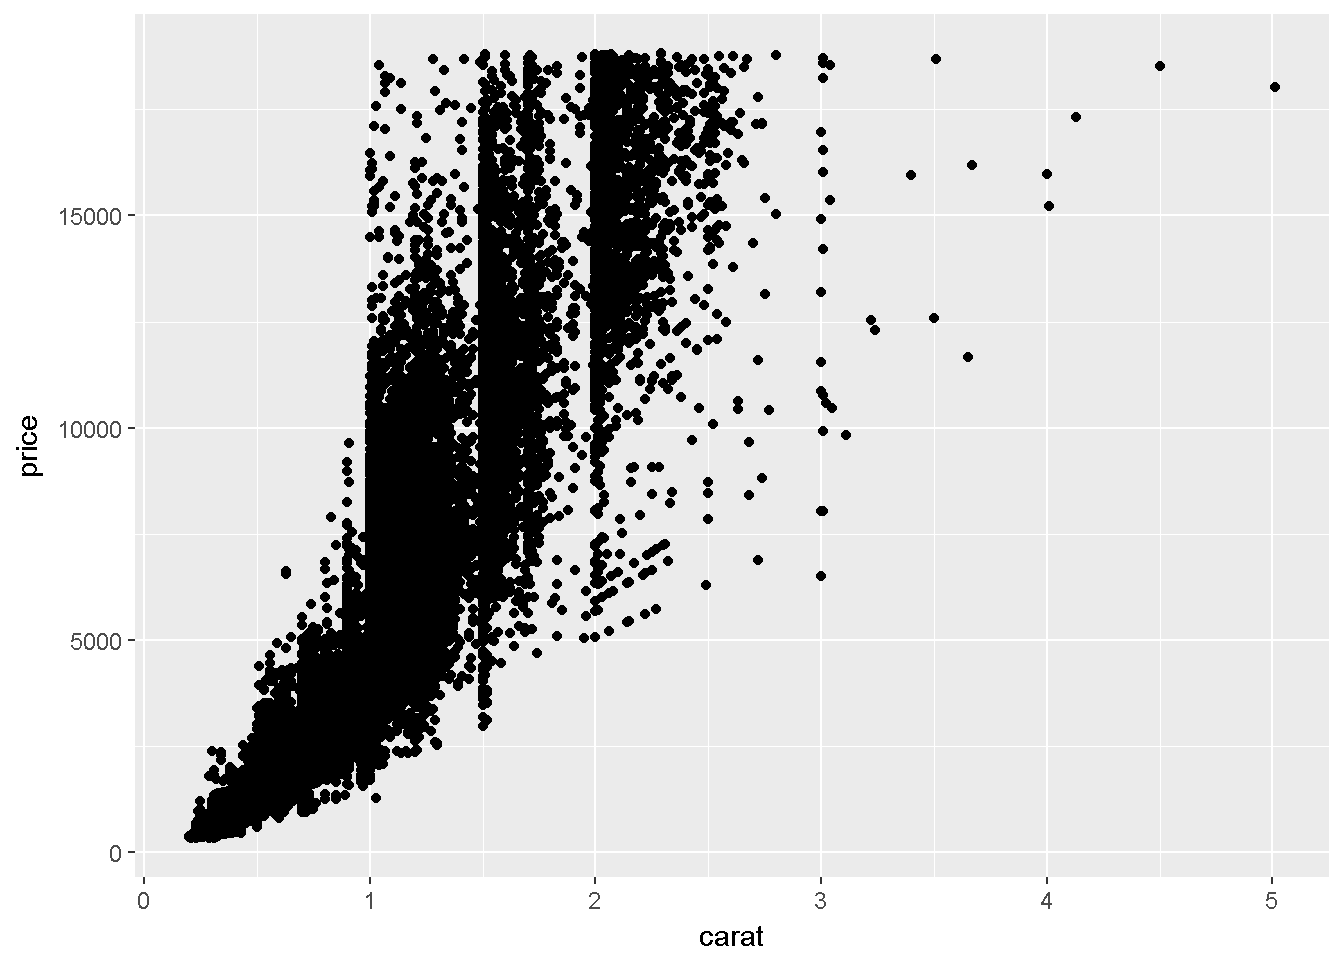
\includegraphics{09-GGPlot_files/figure-latex/p11a-1.pdf}
\caption{\label{fig:p11a}First graph on page 11 of \citet{Wickham2009ggplot2}}
\end{figure}

\begin{Shaded}
\begin{Highlighting}[]
\FunctionTok{VI}\NormalTok{(p11a)  }
\end{Highlighting}
\end{Shaded}

\begin{verbatim}
This is an untitled chart with no subtitle or caption.
It has x-axis 'carat' with labels 0, 1, 2, 3, 4 and 5.
It has y-axis 'price' with labels 0, 5000, 10000 and 15000.
The chart is a set of 53940 points.
\end{verbatim}

Note that unlike some other ways the \texttt{VI()} command has worked, the graph was not created by the nesting of the call to render the graph when nested inside the \texttt{VI()} command. In all the examples that follow, I use the pipe \texttt{\%\textgreater{}\%} operator from the \texttt{magrittr} package to push the graph into the \texttt{VI()} function.

\begin{Shaded}
\begin{Highlighting}[]
\NormalTok{fig2}\FloatTok{.2}\NormalTok{a }\OtherTok{=} \FunctionTok{qplot}\NormalTok{(carat, price, }\AttributeTok{data =}\NormalTok{ dsmall, }\AttributeTok{colour =}\NormalTok{ color)}
\NormalTok{fig2}\FloatTok{.2}\NormalTok{a }\SpecialCharTok{\%\textgreater{}\%} \FunctionTok{VI}\NormalTok{()   }
\end{Highlighting}
\end{Shaded}

\begin{verbatim}
This is an untitled chart with no subtitle or caption.
It has x-axis 'carat' with labels 1, 2, 3 and 4.
It has y-axis 'price' with labels 0, 5000, 10000 and 15000.
There is a legend indicating colour is used to show color, with 7 levels:
D shown as very deep purple colour, 
E shown as vivid purplish blue colour, 
F shown as moderate blue colour, 
G shown as vivid bluish green colour, 
H shown as brilliant green colour, 
I shown as vivid yellow green colour and 
J shown as vivid greenish yellow colour.
The chart is a set of 100 points.
\end{verbatim}

\begin{Shaded}
\begin{Highlighting}[]
\NormalTok{fig2}\FloatTok{.2}\NormalTok{a}
\end{Highlighting}
\end{Shaded}

\begin{figure}
\centering
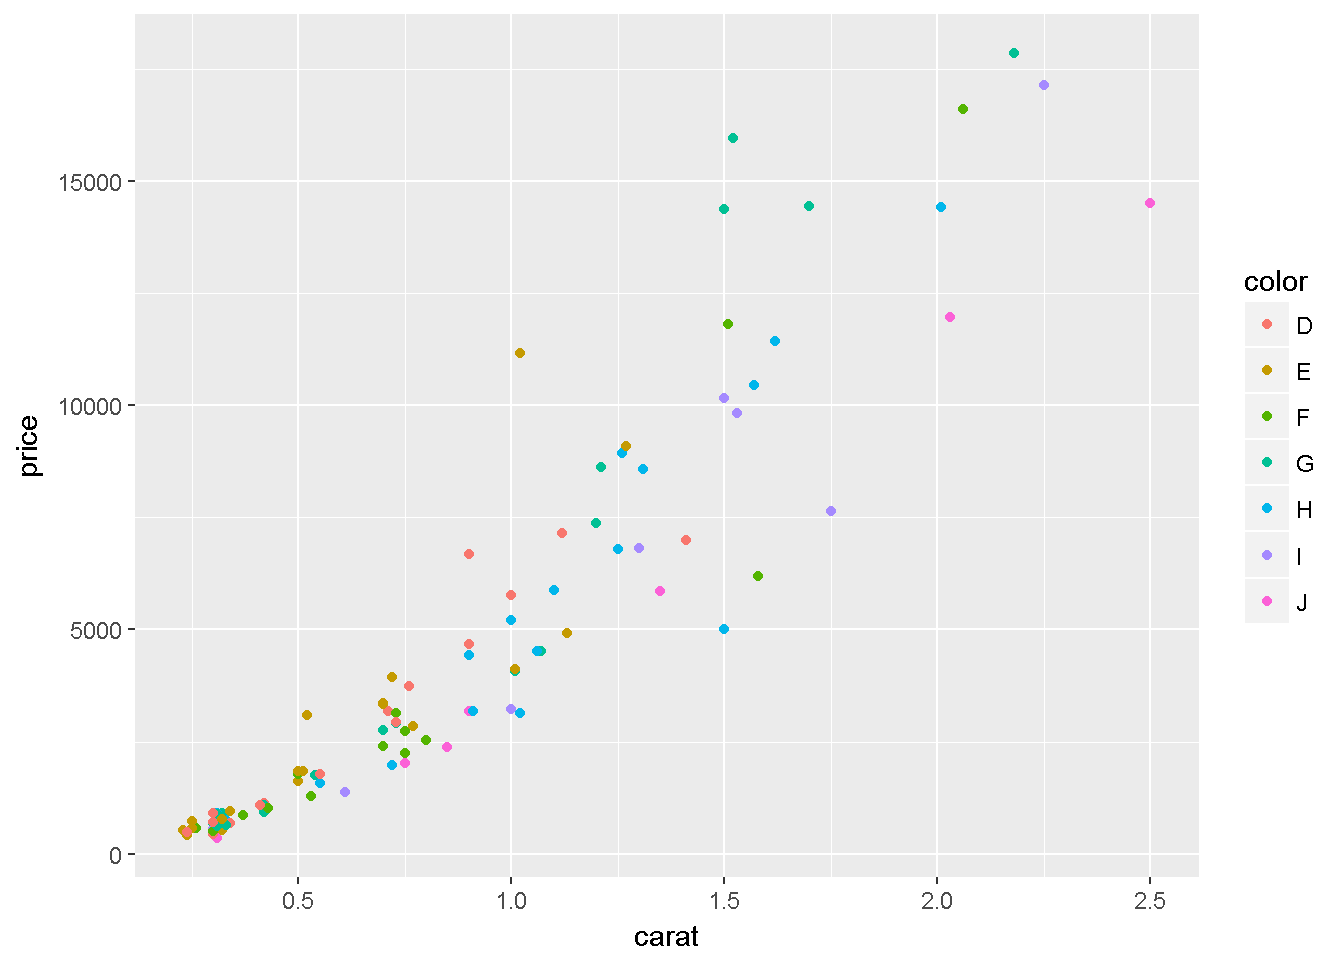
\includegraphics{09-GGPlot_files/figure-latex/fig2-2a-1.pdf}
\caption{\label{fig:fig2-2a}Left pane of Figure 2.2 of \citet{Wickham2009ggplot2}}
\end{figure}

We haven't been able to tell what exact colour was used in the \citet{Wickham2009ggplot2} rendering of this graph, but there has obviously been some minor alteration of the colour palette being used by the \texttt{ggplot2} package.

\begin{Shaded}
\begin{Highlighting}[]
\NormalTok{fig2}\FloatTok{.2}\NormalTok{b }\OtherTok{=} \FunctionTok{qplot}\NormalTok{(carat, price, }\AttributeTok{data =}\NormalTok{ dsmall, }\AttributeTok{shape =}\NormalTok{ cut)    }
\NormalTok{fig2}\FloatTok{.2}\NormalTok{b }\SpecialCharTok{\%\textgreater{}\%} \FunctionTok{VI}\NormalTok{()   }
\end{Highlighting}
\end{Shaded}

\begin{verbatim}
Warning: Using shapes for an ordinal variable is not advised
\end{verbatim}

\begin{verbatim}
This is an untitled chart with no subtitle or caption.
It has x-axis 'carat' with labels 1, 2, 3 and 4.
It has y-axis 'price' with labels 0, 5000, 10000 and 15000.
There is a legend indicating shape is used to show cut, with 5 levels:
Fair shown as solid circle shape, 
Good shown as solid triangle shape, 
Very Good shown as solid square shape, 
Premium shown as plus shape and 
Ideal shown as boxed X shape.
The chart is a set of 100 points.
\end{verbatim}

\begin{Shaded}
\begin{Highlighting}[]
\NormalTok{fig2}\FloatTok{.2}\NormalTok{b}
\end{Highlighting}
\end{Shaded}

\begin{verbatim}
Warning: Using shapes for an ordinal variable is not advised
\end{verbatim}

\begin{figure}
\centering
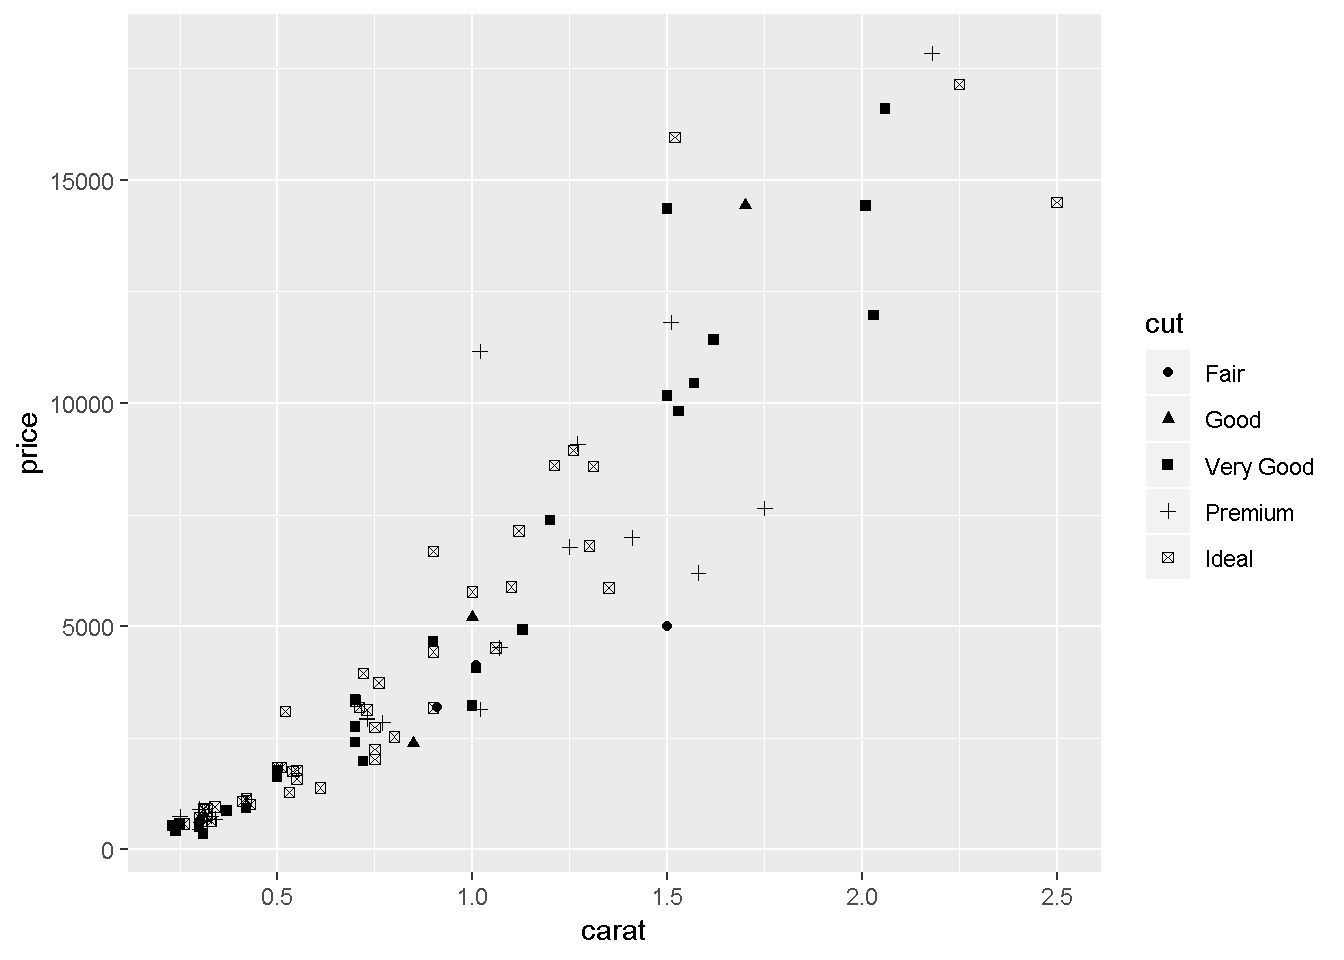
\includegraphics{09-GGPlot_files/figure-latex/fig2-2b-1.pdf}
\caption{\label{fig:fig2-2b}Right pane of Figure 2.2}
\end{figure}

To get semi-transparent points:

\begin{Shaded}
\begin{Highlighting}[]
\NormalTok{fig2}\FloatTok{.3}\NormalTok{b }\OtherTok{=} \FunctionTok{qplot}\NormalTok{(carat, price, }\AttributeTok{data =}\NormalTok{ diamonds, }\AttributeTok{alpha =} \FunctionTok{I}\NormalTok{(}\DecValTok{1}\SpecialCharTok{/}\DecValTok{100}\NormalTok{))    }
\NormalTok{fig2}\FloatTok{.3}\NormalTok{b}
\end{Highlighting}
\end{Shaded}

\begin{figure}
\centering
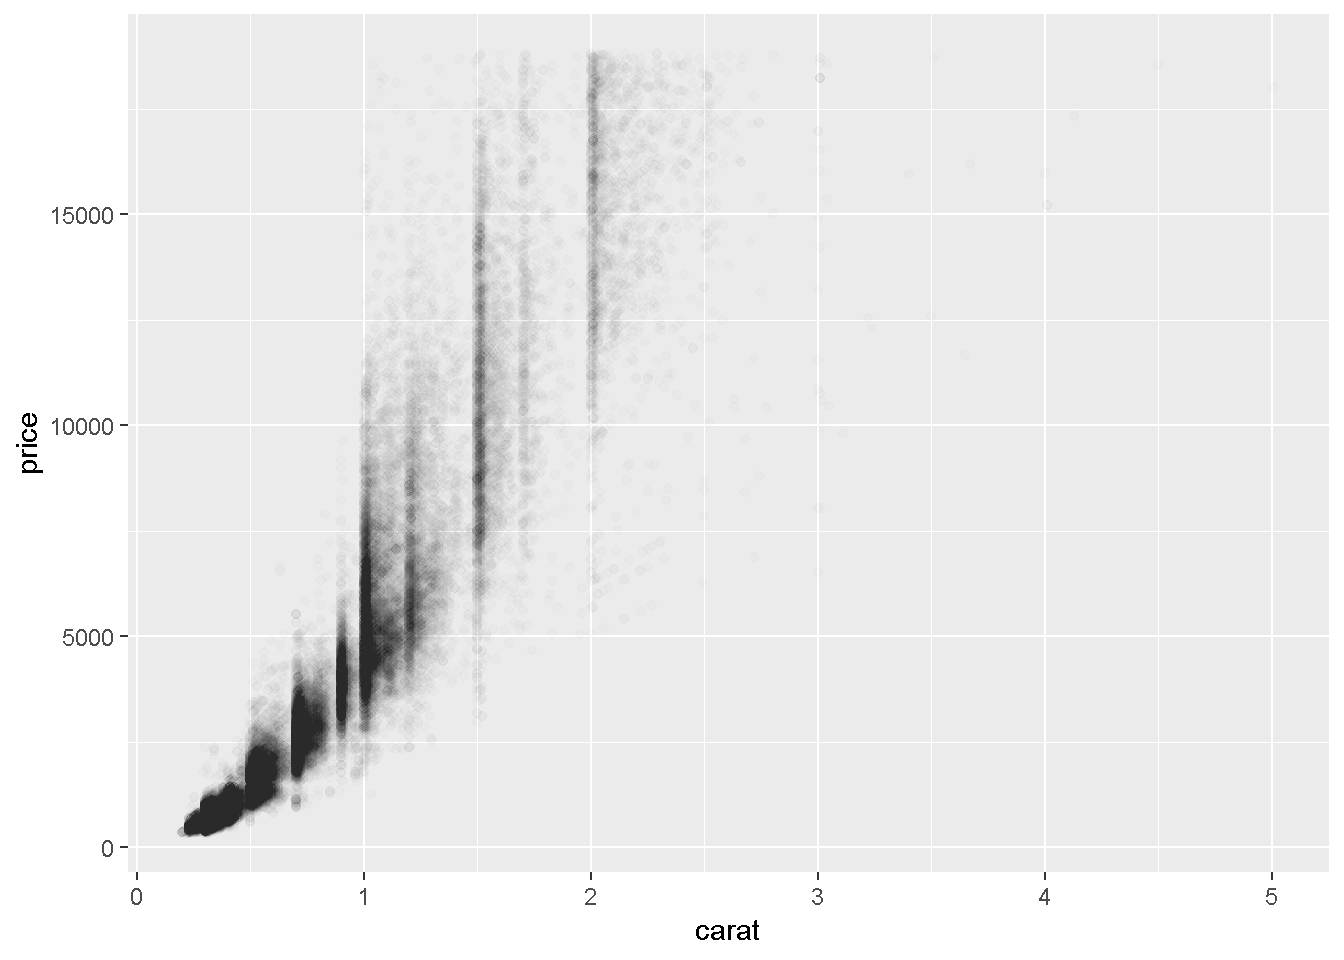
\includegraphics{09-GGPlot_files/figure-latex/fig2-3b-1.pdf}
\caption{\label{fig:fig2-3b}Middle pane from Figure 2.3}
\end{figure}

\begin{Shaded}
\begin{Highlighting}[]
\NormalTok{fig2}\FloatTok{.3}\NormalTok{b }\SpecialCharTok{\%\textgreater{}\%} \FunctionTok{VI}\NormalTok{()   }
\end{Highlighting}
\end{Shaded}

\begin{verbatim}
This is an untitled chart with no subtitle or caption.
It has x-axis 'carat' with labels 0, 1, 2, 3, 4 and 5.
It has y-axis 'price' with labels 0, 5000, 10000 and 15000.
The chart is a set of 53940 points.
It has alpha set to 0.01.
\end{verbatim}

To add a smoother (default is loess for n\textless1000):

\begin{Shaded}
\begin{Highlighting}[]
\NormalTok{fig2}\FloatTok{.4}\NormalTok{a }\OtherTok{=} \FunctionTok{qplot}\NormalTok{(carat, price, }\AttributeTok{data =}\NormalTok{ dsmall, }\AttributeTok{geom =} \FunctionTok{c}\NormalTok{(}\StringTok{"point"}\NormalTok{, }\StringTok{"smooth"}\NormalTok{))    }
\NormalTok{fig2}\FloatTok{.4}\NormalTok{a}
\end{Highlighting}
\end{Shaded}

\begin{verbatim}
`geom_smooth()` using method = 'loess' and formula 'y ~ x'
\end{verbatim}

\begin{figure}
\centering
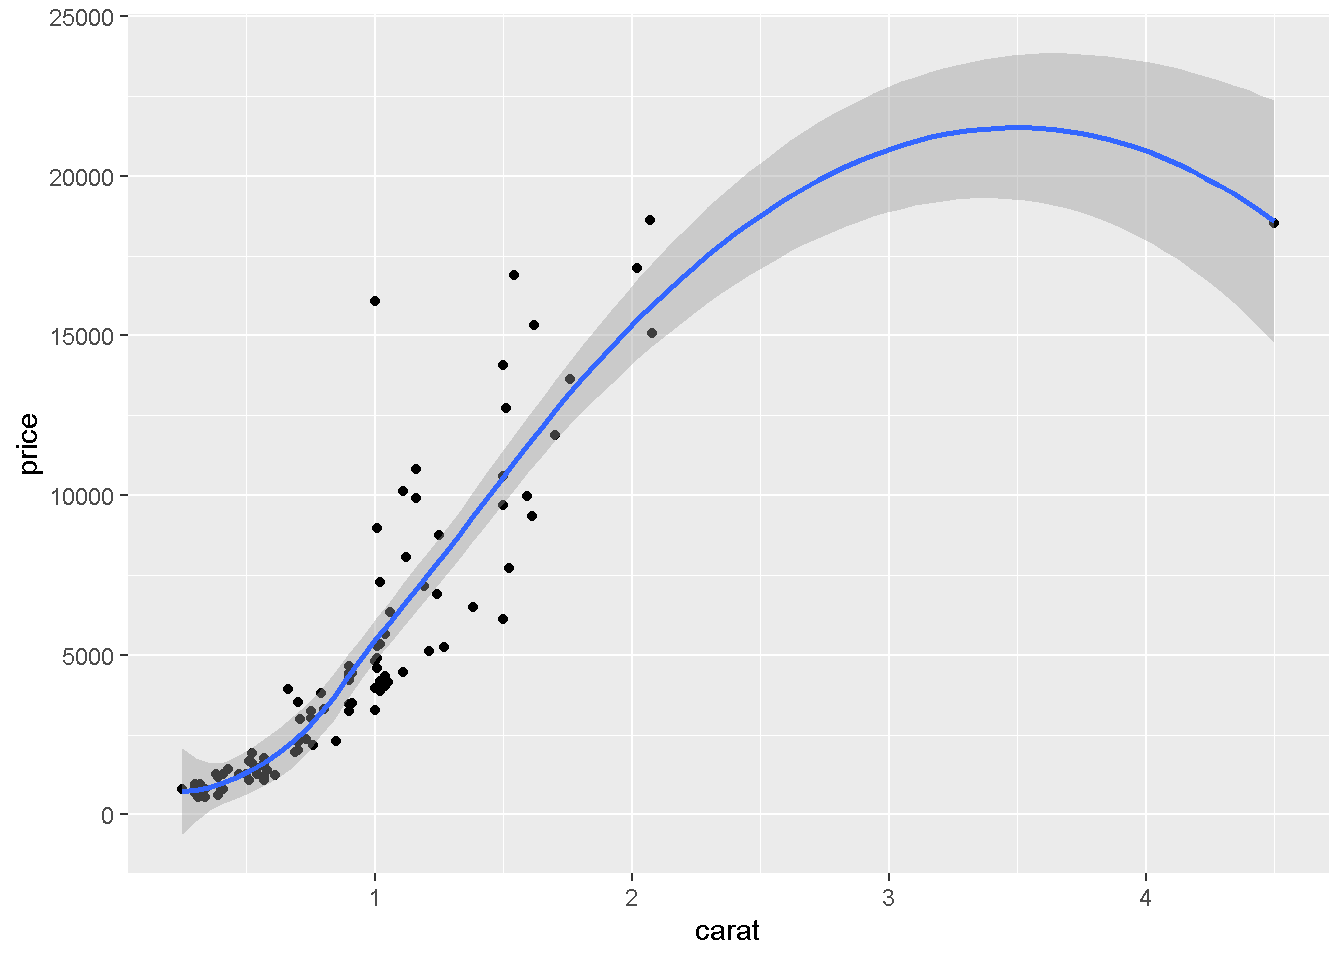
\includegraphics{09-GGPlot_files/figure-latex/fig2-4a-1.pdf}
\caption{\label{fig:fig2-4a}Left pane of Figure 2.4}
\end{figure}

\begin{Shaded}
\begin{Highlighting}[]
\NormalTok{fig2}\FloatTok{.4}\NormalTok{a }\SpecialCharTok{\%\textgreater{}\%} \FunctionTok{VI}\NormalTok{()   }
\end{Highlighting}
\end{Shaded}

\begin{verbatim}
This is an untitled chart with no subtitle or caption.
It has x-axis 'carat' with labels 1, 2, 3 and 4.
It has y-axis 'price' with labels 0, 5000, 10000, 15000, 20000 and 25000.
It has 2 layers.
Layer 1 is a set of 100 points.
Layer 2 is a 'lowess' smoothed curve with 95% confidence intervals.
\end{verbatim}

\hypertarget{plotting-a-continuous-variable-against-a-categorical-variable}{%
\section{Plotting a continuous variable against a categorical variable}\label{plotting-a-continuous-variable-against-a-categorical-variable}}

\begin{Shaded}
\begin{Highlighting}[]
\NormalTok{fig2}\FloatTok{.8}\NormalTok{a  }\OtherTok{=} \FunctionTok{qplot}\NormalTok{(color, price }\SpecialCharTok{/}\NormalTok{ carat, }\AttributeTok{data =}\NormalTok{ diamonds, }\AttributeTok{geom =} \StringTok{"jitter"}\NormalTok{)}
\NormalTok{fig2}\FloatTok{.8}\NormalTok{a}
\end{Highlighting}
\end{Shaded}

\begin{figure}
\centering
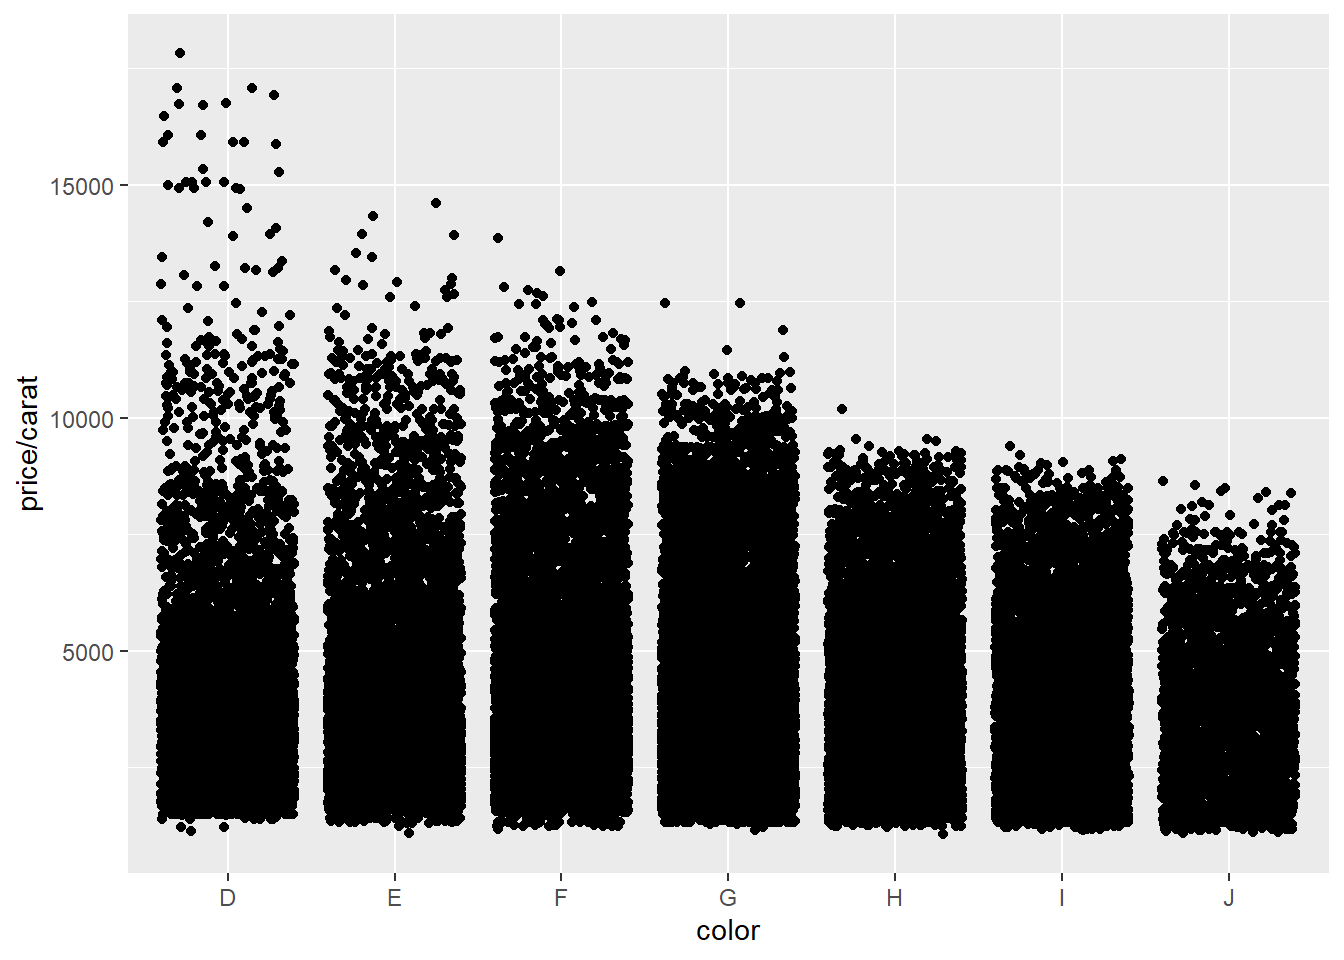
\includegraphics{09-GGPlot_files/figure-latex/fig2-8a-1.pdf}
\caption{\label{fig:fig2-8a}Left pane of Figure 2.8}
\end{figure}

\begin{Shaded}
\begin{Highlighting}[]
\NormalTok{fig2}\FloatTok{.8}\NormalTok{a }\SpecialCharTok{\%\textgreater{}\%} \FunctionTok{VI}\NormalTok{()   }
\end{Highlighting}
\end{Shaded}

\begin{verbatim}
This is an untitled chart with no subtitle or caption.
It has x-axis 'color' with labels D, E, F, G, H, I and J.
It has y-axis 'price/carat' with labels 5000, 10000 and 15000.
The chart is a set of 53940 points.
\end{verbatim}

\begin{Shaded}
\begin{Highlighting}[]
\NormalTok{fig2}\FloatTok{.8}\NormalTok{b }\OtherTok{=} \FunctionTok{qplot}\NormalTok{(color, price }\SpecialCharTok{/}\NormalTok{ carat, }\AttributeTok{data =}\NormalTok{ diamonds, }\AttributeTok{geom =} \StringTok{"boxplot"}\NormalTok{)    }
\NormalTok{fig2}\FloatTok{.8}\NormalTok{b}
\end{Highlighting}
\end{Shaded}

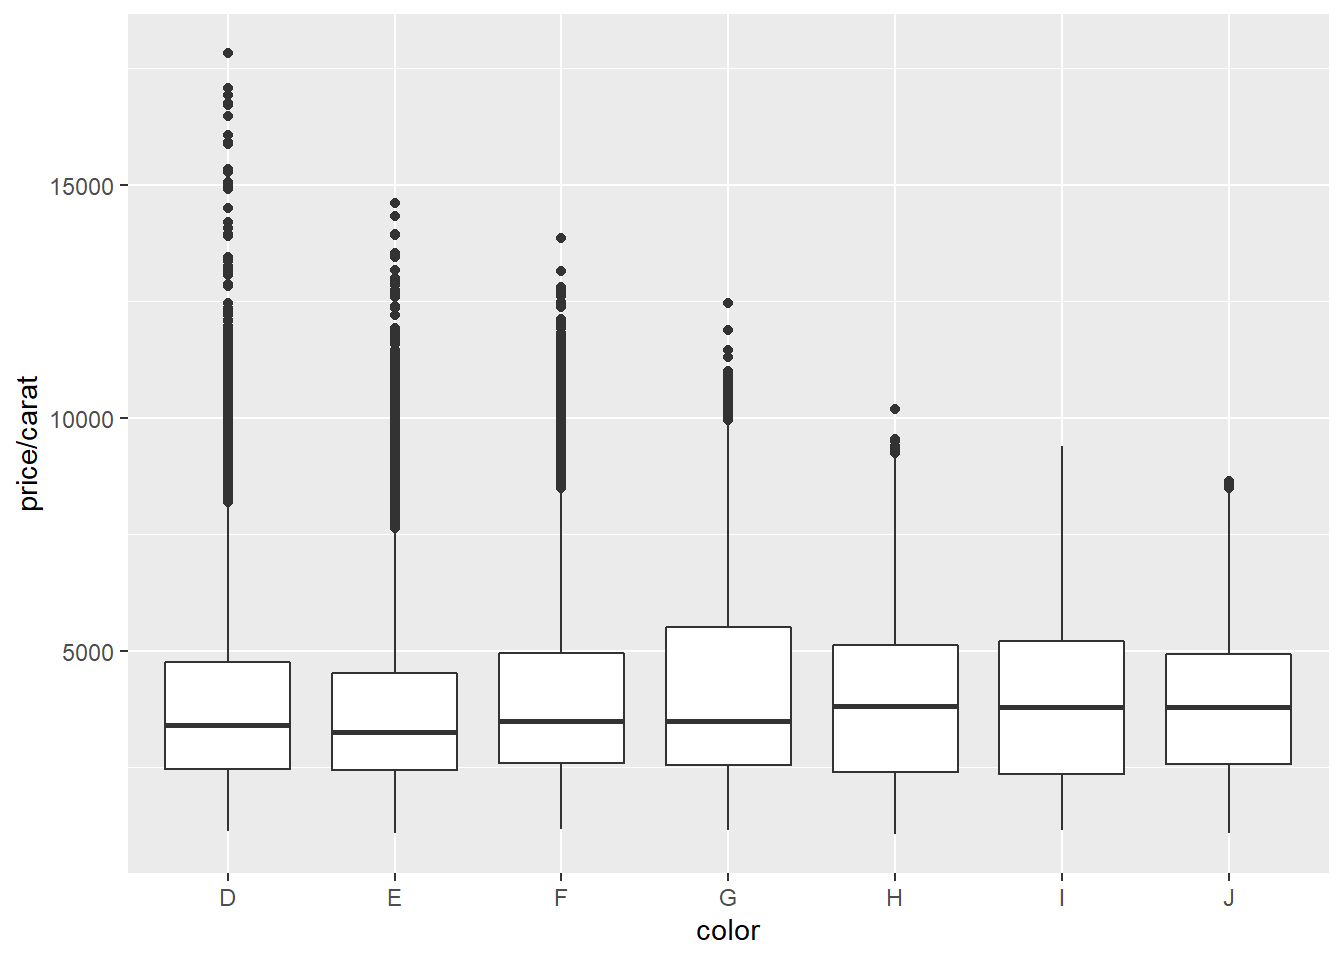
\includegraphics{09-GGPlot_files/figure-latex/fig2-8b-1.pdf}

\begin{Shaded}
\begin{Highlighting}[]
\NormalTok{fig2}\FloatTok{.8}\NormalTok{b }\SpecialCharTok{\%\textgreater{}\%} \FunctionTok{VI}\NormalTok{()   }
\end{Highlighting}
\end{Shaded}

\begin{verbatim}
This is an untitled chart with no subtitle or caption.
It has x-axis 'color' with labels D, E, F, G, H, I and J.
It has y-axis 'price/carat' with labels 5000, 10000 and 15000.
The chart is a boxplot comprised of 7 boxes with whiskers.
There is a box at x=D.
It has median 3410.53. The box goes from 2455 to 4749.31, and the whiskers extend to 1128.12 and 8183.33.
There are 338 outliers for this boxplot.
There is a box at x=E.
It has median 3253.66. The box goes from 2430.3 to 4508.41, and the whiskers extend to 1078.12 and 7616.39.
There are 593 outliers for this boxplot.
There is a box at x=F.
It has median 3494.32. The box goes from 2587.1 to 4947.22, and the whiskers extend to 1168 and 8477.5.
There are 585 outliers for this boxplot.
There is a box at x=G.
It has median 3490.38. The box goes from 2538.24 to 5500, and the whiskers extend to 1139.02 and 9937.2.
There are 119 outliers for this boxplot.
There is a box at x=H.
It has median 3818.89. The box goes from 2396.88 to 5127.28, and the whiskers extend to 1051.16 and 9220.
There are 13 outliers for this boxplot.
There is a box at x=I.
It has median 3779.74. The box goes from 2344.65 to 5196.75, and the whiskers extend to 1151.72 and 9397.5.
There are 0 outliers for this boxplot.
There is a box at x=J.
It has median 3780. The box goes from 2562.87 to 4927.95, and the whiskers extend to 1080.65 and 8426.13.
There are 3 outliers for this boxplot.
\end{verbatim}

When seeking to use shading or opaqueness to describe the density of the points, the fact the size of the points has an impact on the opaqueness is not currently realised by \texttt{BrailleR}.

\begin{Shaded}
\begin{Highlighting}[]
\NormalTok{fig2}\FloatTok{.9}\NormalTok{b }\OtherTok{=} \FunctionTok{qplot}\NormalTok{(color, price }\SpecialCharTok{/}\NormalTok{ carat, }\AttributeTok{data =}\NormalTok{ diamonds, }\AttributeTok{geom =} \StringTok{"jitter"}\NormalTok{, }\AttributeTok{alpha =} \FunctionTok{I}\NormalTok{(}\DecValTok{1} \SpecialCharTok{/} \DecValTok{50}\NormalTok{))    }
\NormalTok{fig2}\FloatTok{.9}\NormalTok{b}
\end{Highlighting}
\end{Shaded}

\begin{figure}
\centering
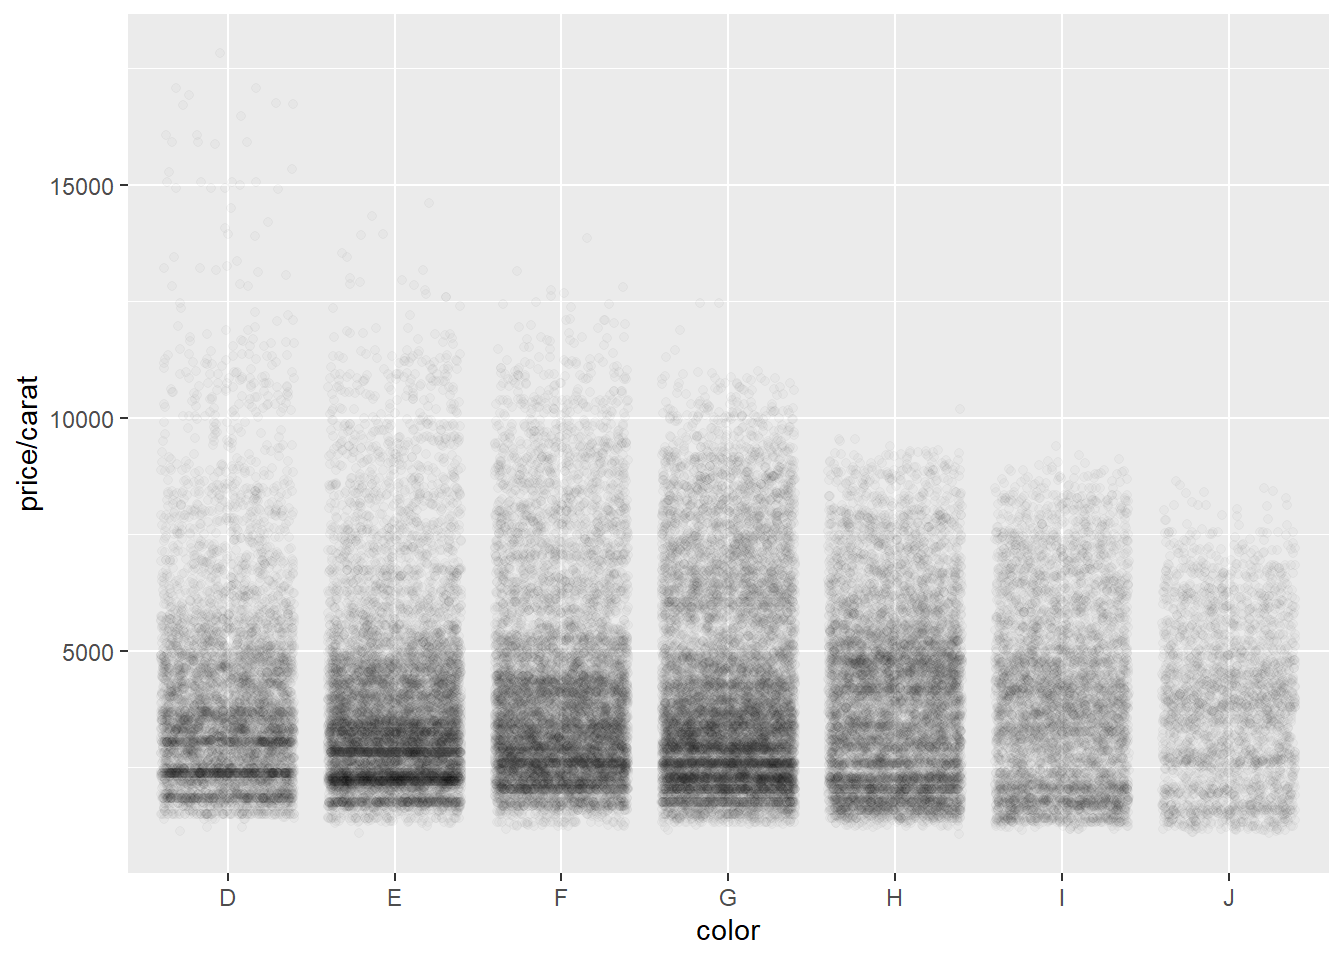
\includegraphics{09-GGPlot_files/figure-latex/fig2-9b-1.pdf}
\caption{\label{fig:fig2-9b}Middle pane of Figure 2.9}
\end{figure}

\begin{Shaded}
\begin{Highlighting}[]
\NormalTok{fig2}\FloatTok{.9}\NormalTok{b }\SpecialCharTok{\%\textgreater{}\%} \FunctionTok{VI}\NormalTok{()   }
\end{Highlighting}
\end{Shaded}

\begin{verbatim}
This is an untitled chart with no subtitle or caption.
It has x-axis 'color' with labels D, E, F, G, H, I and J.
It has y-axis 'price/carat' with labels 5000, 10000 and 15000.
The chart is a set of 53940 points.
It has alpha set to 0.02.
\end{verbatim}

\hypertarget{univariate-plots}{%
\subsection{Univariate plots}\label{univariate-plots}}

\begin{Shaded}
\begin{Highlighting}[]
\NormalTok{fig2}\FloatTok{.10}\NormalTok{a }\OtherTok{=} \FunctionTok{qplot}\NormalTok{(carat, }\AttributeTok{data =}\NormalTok{ diamonds, }\AttributeTok{geom =} \StringTok{"histogram"}\NormalTok{)    }
\NormalTok{fig2}\FloatTok{.10}\NormalTok{a}
\end{Highlighting}
\end{Shaded}

\begin{verbatim}
`stat_bin()` using `bins = 30`. Pick better value with `binwidth`.
\end{verbatim}

\begin{figure}
\centering
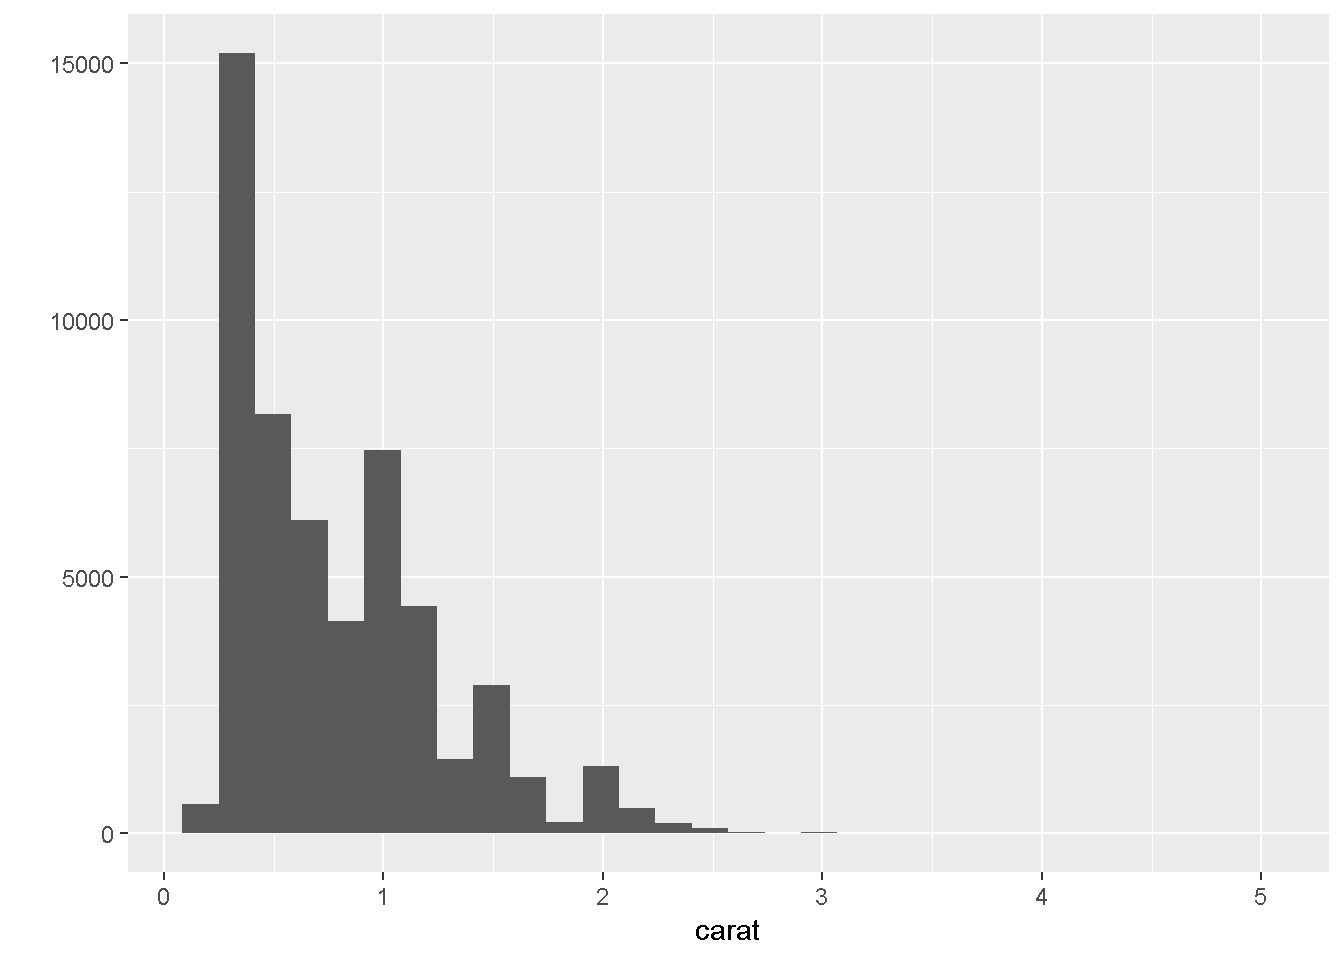
\includegraphics{09-GGPlot_files/figure-latex/fig2-10a-1.pdf}
\caption{\label{fig:fig2-10a}Left pane of Figure 2.10}
\end{figure}

\begin{Shaded}
\begin{Highlighting}[]
\NormalTok{fig2}\FloatTok{.10}\NormalTok{a }\SpecialCharTok{\%\textgreater{}\%} \FunctionTok{VI}\NormalTok{()   }
\end{Highlighting}
\end{Shaded}

\begin{verbatim}
This is an untitled chart with no subtitle or caption.
It has x-axis 'carat' with labels 0, 1, 2, 3, 4 and 5.
It has y-axis '' with labels 0, 5000, 10000 and 15000.
The chart is a bar chart with 30 vertical bars.
\end{verbatim}

Warning: This figure does look different to the original in \citet{Wickham2009ggplot2} ins spite of using the same code and same data.

\begin{Shaded}
\begin{Highlighting}[]
\NormalTok{fig2}\FloatTok{.10}\NormalTok{b }\OtherTok{=} \FunctionTok{qplot}\NormalTok{(carat, }\AttributeTok{data =}\NormalTok{ diamonds, }\AttributeTok{geom =} \StringTok{"density"}\NormalTok{)    }
\NormalTok{fig2}\FloatTok{.10}\NormalTok{b}
\end{Highlighting}
\end{Shaded}

\begin{figure}
\centering
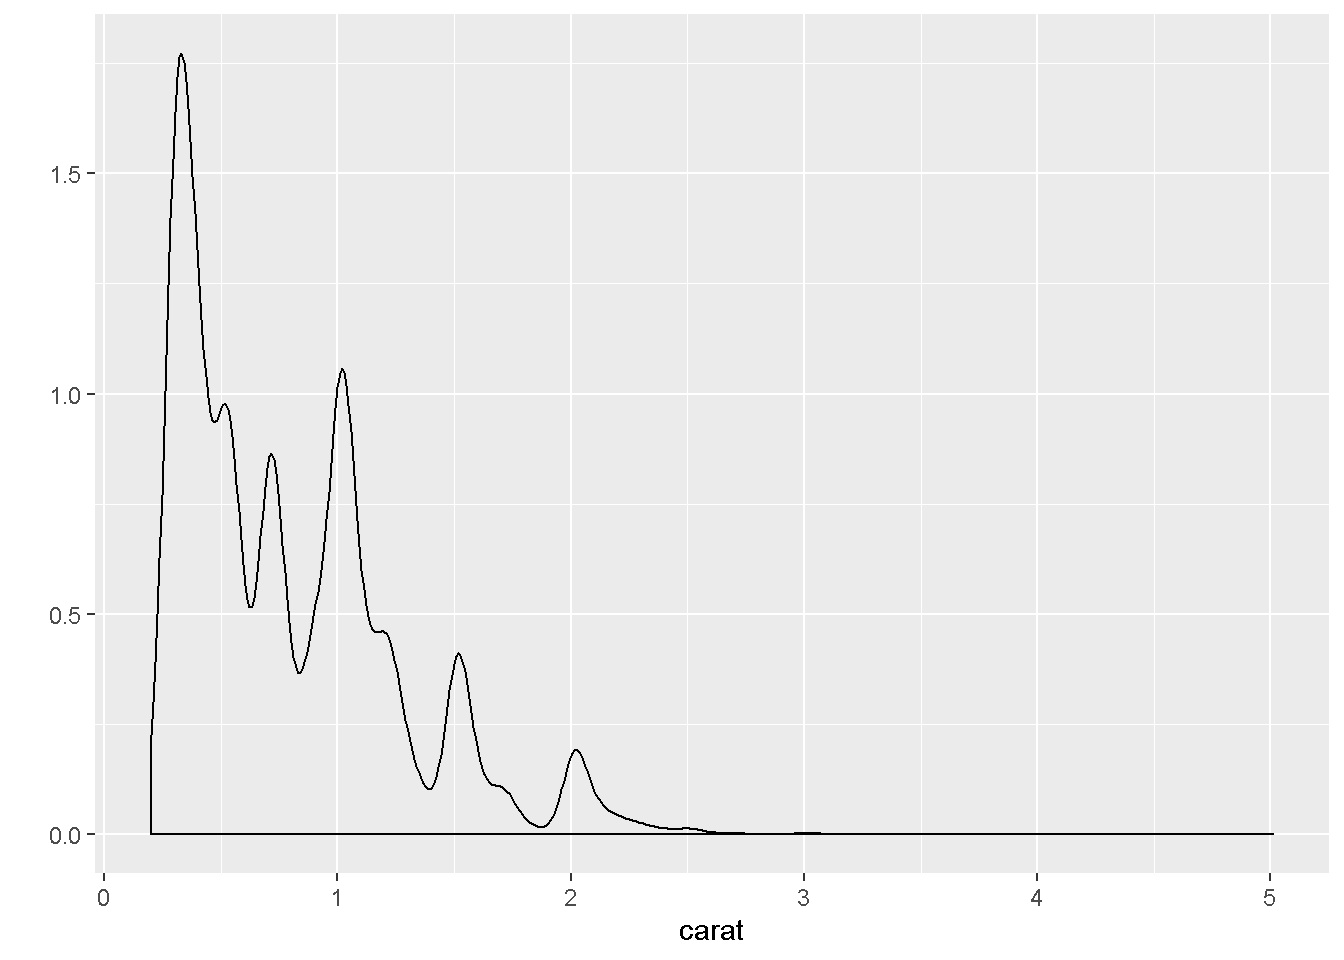
\includegraphics{09-GGPlot_files/figure-latex/fig2-10b-1.pdf}
\caption{\label{fig:fig2-10b}Right pane of Figure 2.10}
\end{figure}

\begin{Shaded}
\begin{Highlighting}[]
\NormalTok{fig2}\FloatTok{.10}\NormalTok{b }\SpecialCharTok{\%\textgreater{}\%} \FunctionTok{VI}\NormalTok{()   }
\end{Highlighting}
\end{Shaded}

\begin{verbatim}
This is an untitled chart with no subtitle or caption.
It has x-axis 'carat' with labels 0, 1, 2, 3, 4 and 5.
It has y-axis '' with labels 0.0, 0.5, 1.0 and 1.5.
The chart is a density graph that VI can not process.
\end{verbatim}

\begin{Shaded}
\begin{Highlighting}[]
\NormalTok{fig2}\FloatTok{.11}\NormalTok{c }\OtherTok{=} \FunctionTok{qplot}\NormalTok{(carat, }\AttributeTok{data =}\NormalTok{ diamonds, }\AttributeTok{geom =} \StringTok{"histogram"}\NormalTok{, }\AttributeTok{binwidth =} \FloatTok{0.01}\NormalTok{, }\AttributeTok{xlim =} \FunctionTok{c}\NormalTok{(}\DecValTok{0}\NormalTok{,}\DecValTok{3}\NormalTok{))    }
\NormalTok{fig2}\FloatTok{.11}\NormalTok{c}
\end{Highlighting}
\end{Shaded}

\begin{verbatim}
Warning: Removed 32 rows containing non-finite values (stat_bin).
\end{verbatim}

\begin{verbatim}
Warning: Removed 2 rows containing missing values (geom_bar).
\end{verbatim}

\begin{figure}
\centering
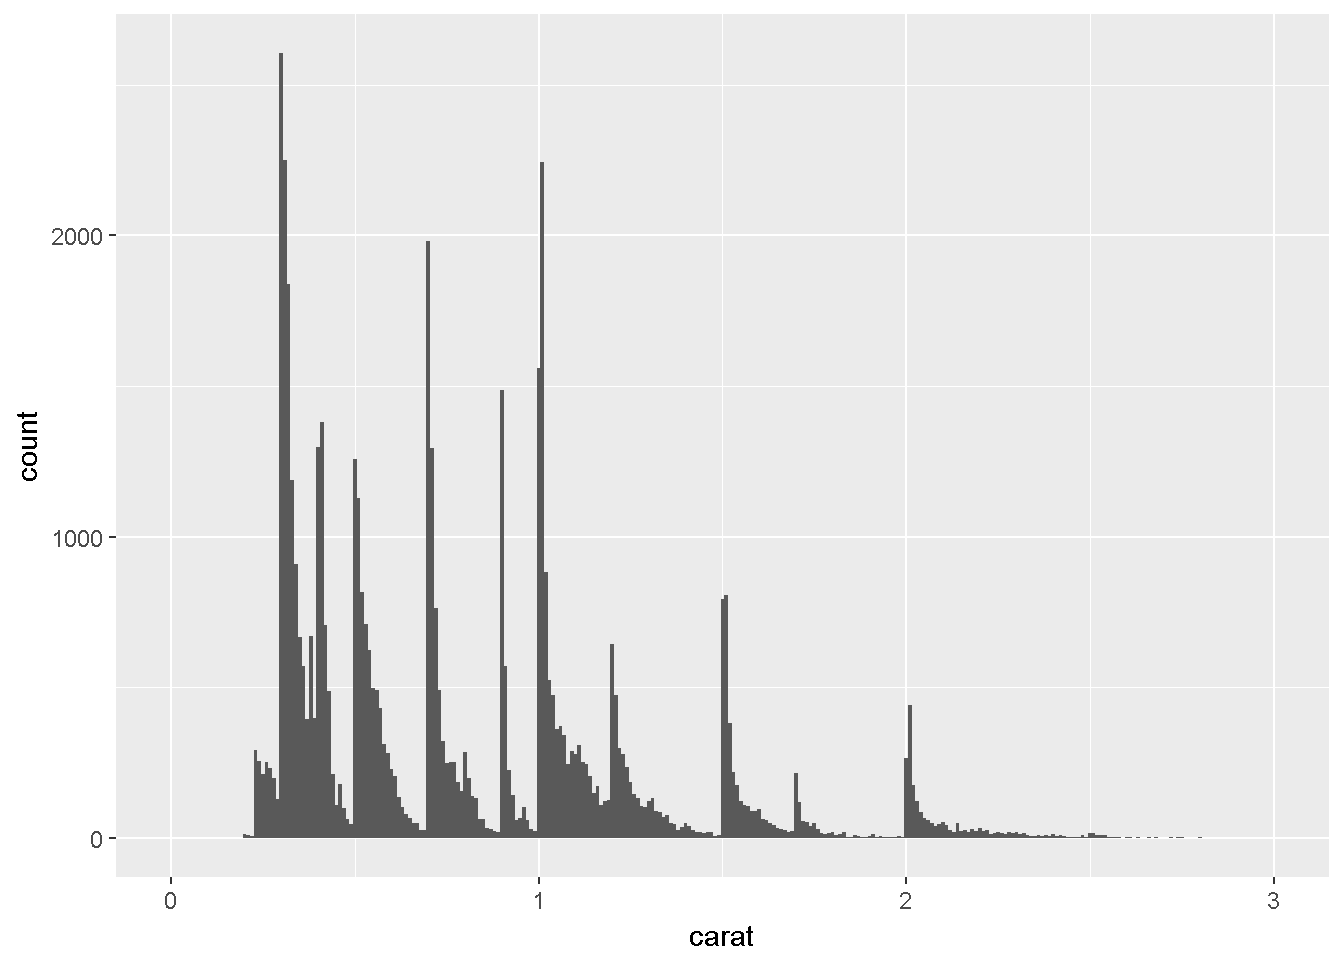
\includegraphics{09-GGPlot_files/figure-latex/fig2-11c-1.pdf}
\caption{\label{fig:fig2-11c}Right pane of Figure 2.11}
\end{figure}

\begin{Shaded}
\begin{Highlighting}[]
\NormalTok{fig2}\FloatTok{.11}\NormalTok{c }\SpecialCharTok{\%\textgreater{}\%} \FunctionTok{VI}\NormalTok{()   }
\end{Highlighting}
\end{Shaded}

\begin{verbatim}
Warning: Removed 32 rows containing non-finite values (stat_bin).
\end{verbatim}

\begin{verbatim}
This is an untitled chart with no subtitle or caption.
It has x-axis 'carat' with labels 0, 1, 2 and 3.
It has y-axis '' with labels 0, 1000 and 2000.
The chart is a bar chart with 299 vertical bars.
\end{verbatim}

The data is separated by implication in the following graphs. The legend is automatically generated and has altered in appearance since the original was produced in \citet{Wickham2009ggplot2}.

\begin{Shaded}
\begin{Highlighting}[]
\NormalTok{fig2}\FloatTok{.12}\NormalTok{a }\OtherTok{=} \FunctionTok{qplot}\NormalTok{(carat, }\AttributeTok{data =}\NormalTok{ diamonds, }\AttributeTok{geom =} \StringTok{"density"}\NormalTok{, }\AttributeTok{colour =}\NormalTok{ color)    }
\NormalTok{fig2}\FloatTok{.12}\NormalTok{a}
\end{Highlighting}
\end{Shaded}

\begin{figure}
\centering
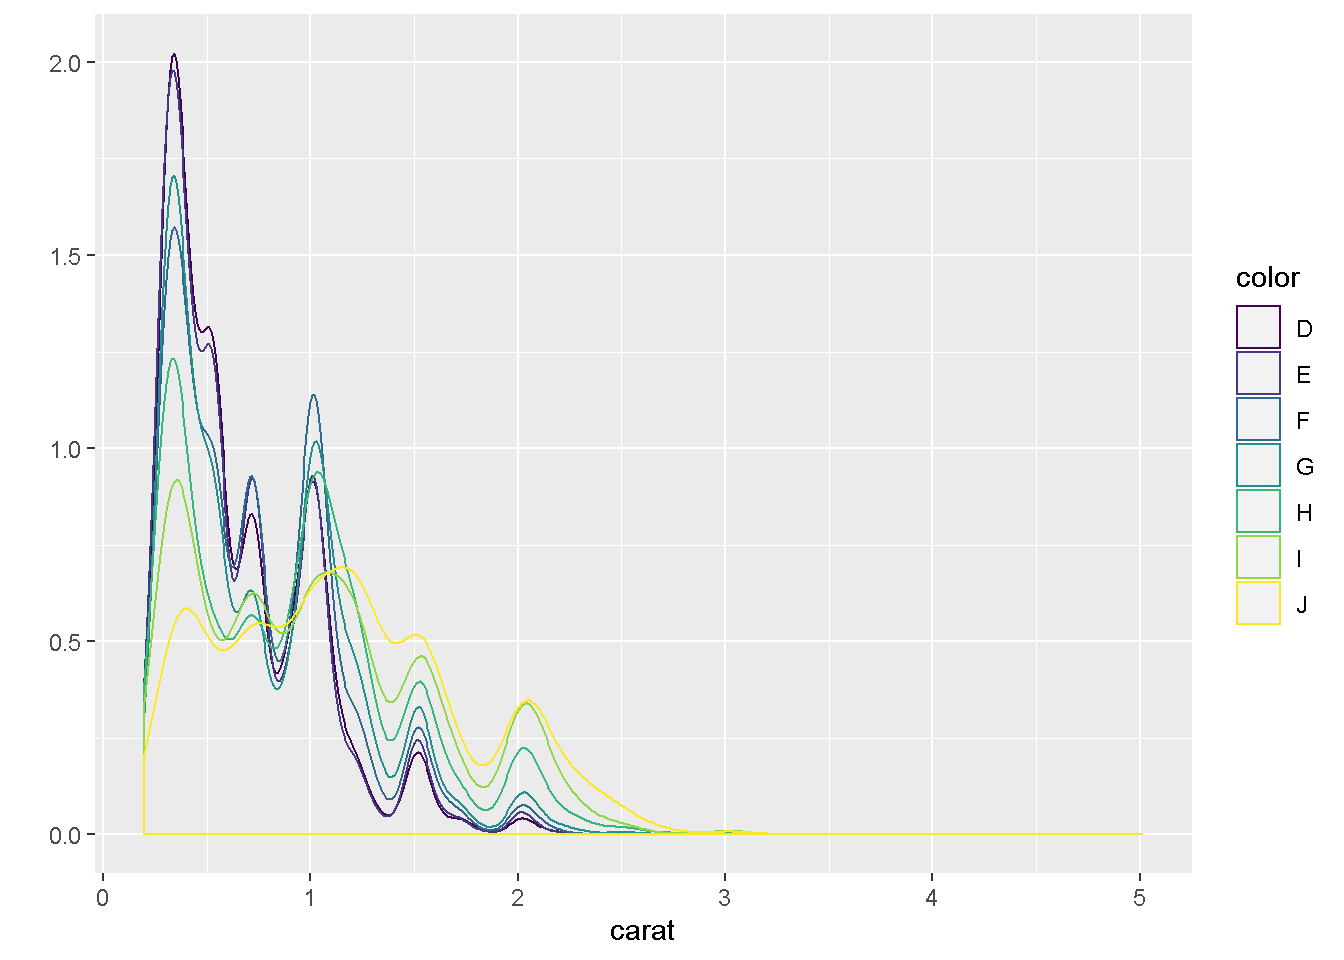
\includegraphics{09-GGPlot_files/figure-latex/fig2-12a-1.pdf}
\caption{\label{fig:fig2-12a}Left pane of Figure 2.12}
\end{figure}

\begin{Shaded}
\begin{Highlighting}[]
\NormalTok{fig2}\FloatTok{.12}\NormalTok{a }\SpecialCharTok{\%\textgreater{}\%} \FunctionTok{VI}\NormalTok{()   }
\end{Highlighting}
\end{Shaded}

\begin{verbatim}
This is an untitled chart with no subtitle or caption.
It has x-axis 'carat' with labels 0, 1, 2, 3, 4 and 5.
It has y-axis '' with labels 0.0, 0.5, 1.0, 1.5 and 2.0.
There is a legend indicating colour is used to show color, with 7 levels:
D shown as very deep purple colour, 
E shown as vivid purplish blue colour, 
F shown as moderate blue colour, 
G shown as vivid bluish green colour, 
H shown as brilliant green colour, 
I shown as vivid yellow green colour and 
J shown as vivid greenish yellow colour.
The chart is a density graph that VI can not process.
\end{verbatim}

\begin{Shaded}
\begin{Highlighting}[]
\NormalTok{fig2}\FloatTok{.12}\NormalTok{b }\OtherTok{=} \FunctionTok{qplot}\NormalTok{(carat, }\AttributeTok{data =}\NormalTok{ diamonds, }\AttributeTok{geom =} \StringTok{"histogram"}\NormalTok{, }\AttributeTok{fill =}\NormalTok{ color)    }
\NormalTok{fig2}\FloatTok{.12}\NormalTok{b}
\end{Highlighting}
\end{Shaded}

\begin{verbatim}
`stat_bin()` using `bins = 30`. Pick better value with `binwidth`.
\end{verbatim}

\begin{figure}
\centering
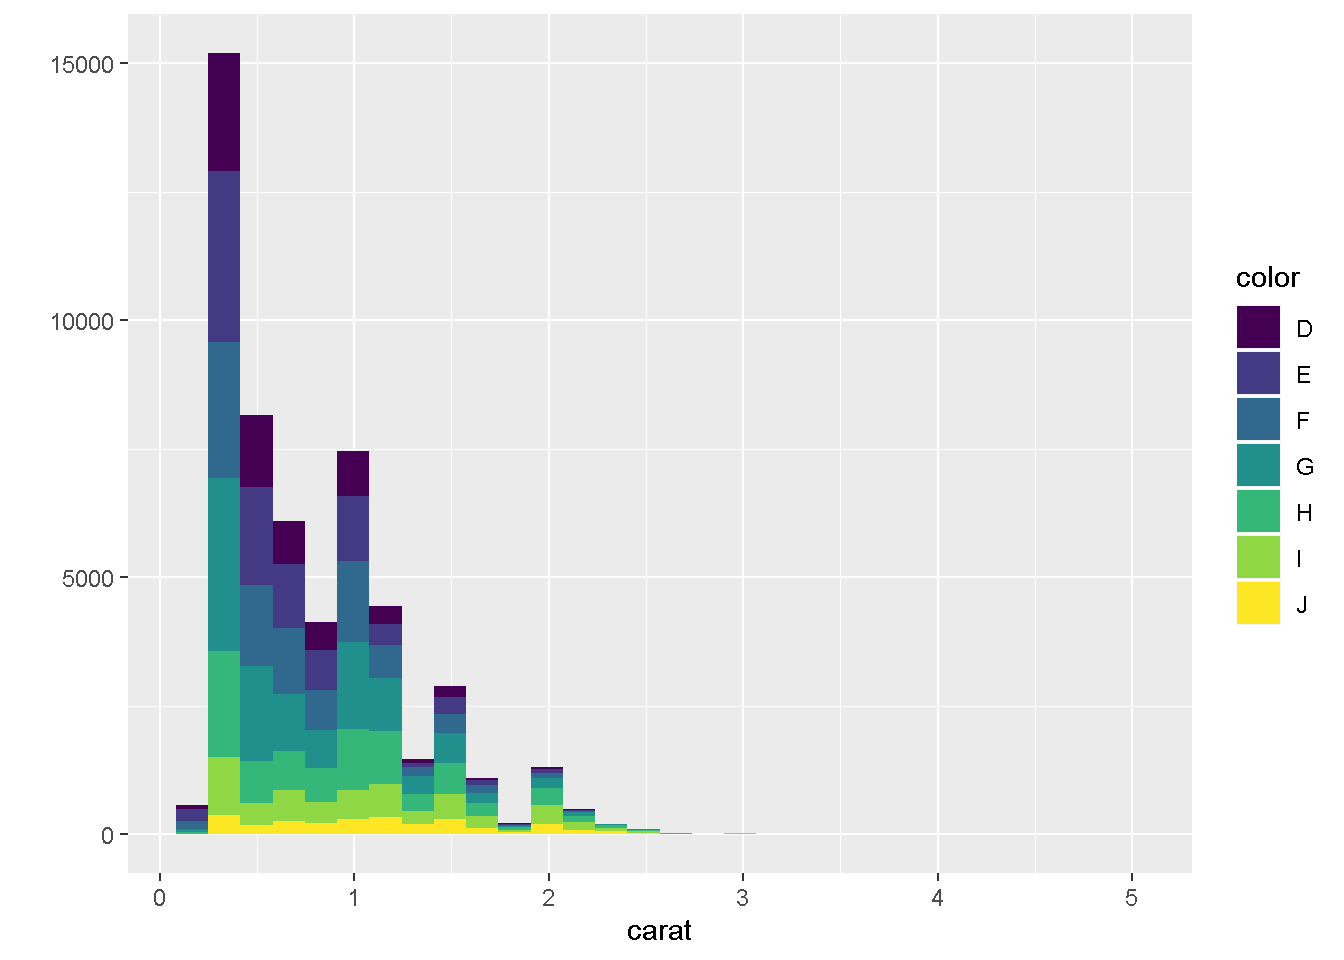
\includegraphics{09-GGPlot_files/figure-latex/fig2-12b-1.pdf}
\caption{\label{fig:fig2-12b}Right pane of Figure 2.12}
\end{figure}

\begin{Shaded}
\begin{Highlighting}[]
\NormalTok{fig2}\FloatTok{.12}\NormalTok{b }\SpecialCharTok{\%\textgreater{}\%} \FunctionTok{VI}\NormalTok{()   }
\end{Highlighting}
\end{Shaded}

\begin{verbatim}
This is an untitled chart with no subtitle or caption.
It has x-axis 'carat' with labels 0, 1, 2, 3, 4 and 5.
It has y-axis '' with labels 0, 5000, 10000 and 15000.
There is a legend indicating fill is used to show color, with 7 levels:
D shown as very deep purple fill, 
E shown as vivid purplish blue fill, 
F shown as moderate blue fill, 
G shown as vivid bluish green fill, 
H shown as brilliant green fill, 
I shown as vivid yellow green fill and 
J shown as vivid greenish yellow fill.
The chart is a bar chart with 210 vertical bars.
These are stacked, as sorted by color.
\end{verbatim}

\hypertarget{bar-charts-for-categorical-variables}{%
\subsection{Bar charts for categorical variables}\label{bar-charts-for-categorical-variables}}

\begin{Shaded}
\begin{Highlighting}[]
\NormalTok{fig2}\FloatTok{.13}\NormalTok{a  }\OtherTok{=} \FunctionTok{qplot}\NormalTok{(color, }\AttributeTok{data =}\NormalTok{ diamonds, }\AttributeTok{geom =} \StringTok{"bar"}\NormalTok{) }\CommentTok{\#geom="bar" is the default    }
\NormalTok{fig2}\FloatTok{.13}\NormalTok{a}
\end{Highlighting}
\end{Shaded}

\begin{figure}
\centering
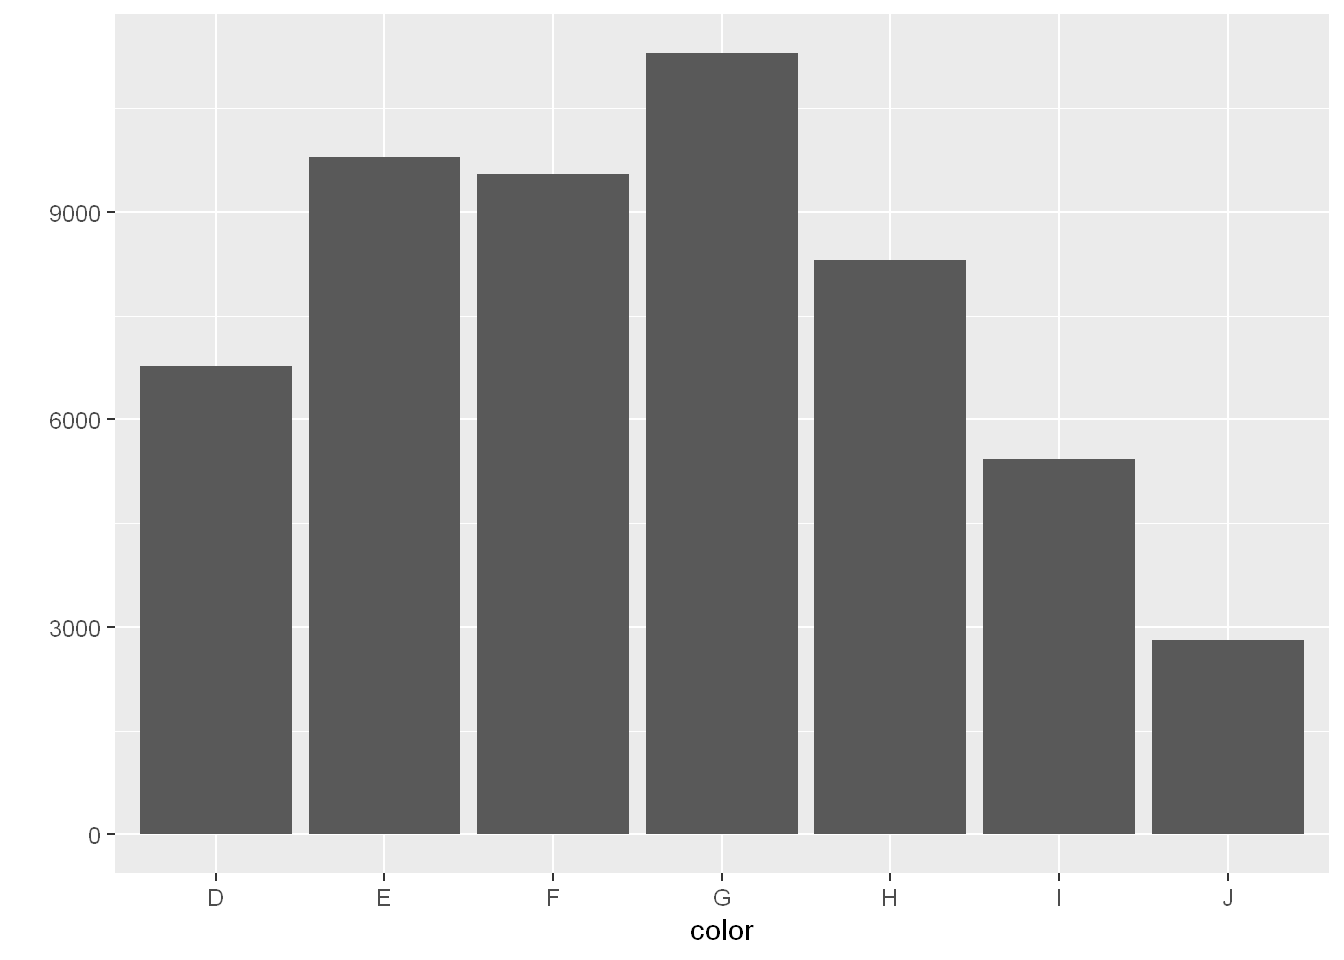
\includegraphics{09-GGPlot_files/figure-latex/fig2-13a-1.pdf}
\caption{\label{fig:fig2-13a}Left pane of Figure 2.13}
\end{figure}

\begin{Shaded}
\begin{Highlighting}[]
\NormalTok{fig2}\FloatTok{.13}\NormalTok{a }\SpecialCharTok{\%\textgreater{}\%} \FunctionTok{VI}\NormalTok{()   }
\end{Highlighting}
\end{Shaded}

\begin{verbatim}
This is an untitled chart with no subtitle or caption.
It has x-axis 'color' with labels D, E, F, G, H, I and J.
It has y-axis '' with labels 0, 3000, 6000 and 9000.
The chart is a bar chart with 7 vertical bars.
Bar 1 is centered horizontally at D, and spans vertically from 0 to 6775.
Bar 2 is centered horizontally at E, and spans vertically from 0 to 9797.
Bar 3 is centered horizontally at F, and spans vertically from 0 to 9542.
Bar 4 is centered horizontally at G, and spans vertically from 0 to 11292.
Bar 5 is centered horizontally at H, and spans vertically from 0 to 8304.
Bar 6 is centered horizontally at I, and spans vertically from 0 to 5422.
Bar 7 is centered horizontally at J, and spans vertically from 0 to 2808.
\end{verbatim}

need to check\ldots{}

\begin{Shaded}
\begin{Highlighting}[]
\NormalTok{fig2}\FloatTok{.13}\NormalTok{b }\OtherTok{=} \FunctionTok{qplot}\NormalTok{(color, }\AttributeTok{data =}\NormalTok{ diamonds, }\AttributeTok{geom =} \StringTok{"bar"}\NormalTok{, }\AttributeTok{weight =}\NormalTok{ carat)   }
\NormalTok{fig2}\FloatTok{.13}\NormalTok{b}
\end{Highlighting}
\end{Shaded}

\begin{figure}
\centering
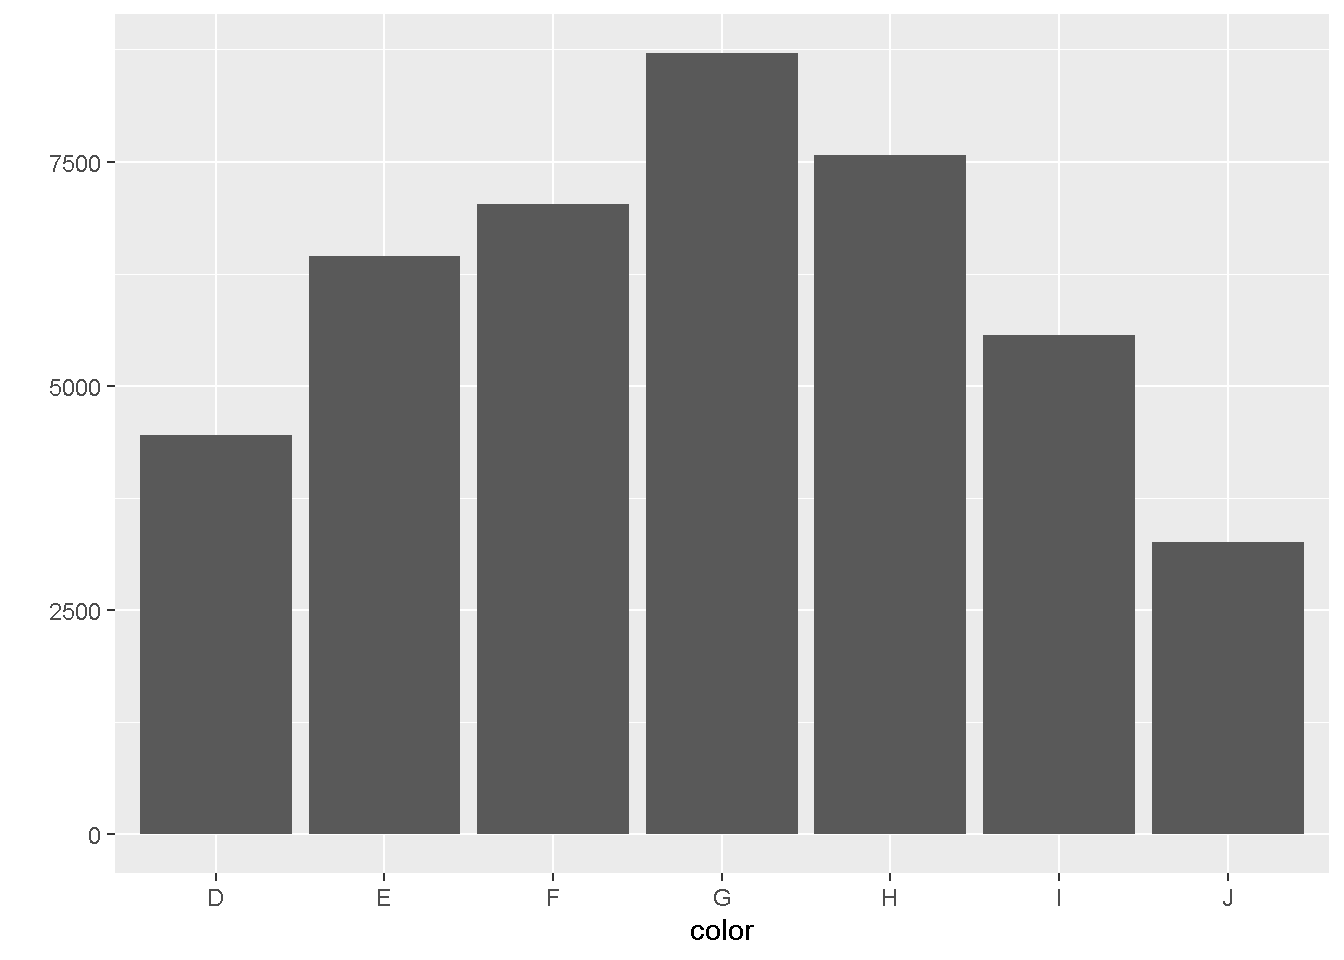
\includegraphics{09-GGPlot_files/figure-latex/fig2-13b-1.pdf}
\caption{\label{fig:fig2-13b-1}Right pane of Figure 2.13}
\end{figure}

\begin{Shaded}
\begin{Highlighting}[]
\NormalTok{fig2}\FloatTok{.13}\NormalTok{b }\OtherTok{=} \FunctionTok{qplot}\NormalTok{(color, }\AttributeTok{data =}\NormalTok{ diamonds, }\AttributeTok{geom =} \StringTok{"bar"}\NormalTok{, }\AttributeTok{weight =}\NormalTok{ carat) }\SpecialCharTok{+} \FunctionTok{scale\_y\_continuous}\NormalTok{(}\StringTok{"carat"}\NormalTok{)    }
\NormalTok{fig2}\FloatTok{.13}\NormalTok{b}
\end{Highlighting}
\end{Shaded}

\begin{figure}
\centering
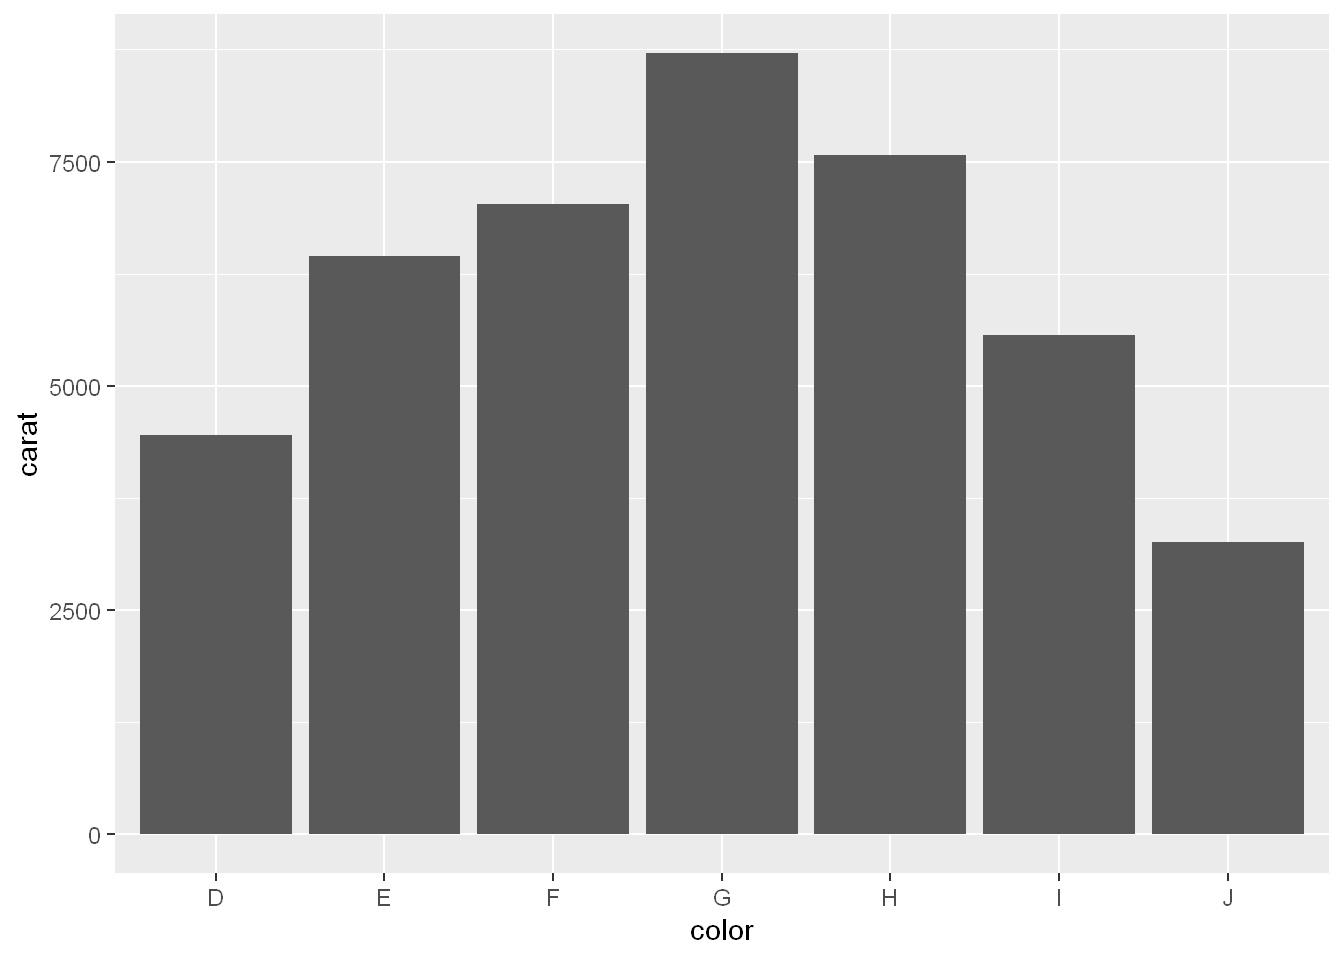
\includegraphics{09-GGPlot_files/figure-latex/fig2-13b-2.pdf}
\caption{\label{fig:fig2-13b-2}Right pane of Figure 2.13}
\end{figure}

\begin{Shaded}
\begin{Highlighting}[]
\NormalTok{fig2}\FloatTok{.13}\NormalTok{b }\SpecialCharTok{\%\textgreater{}\%} \FunctionTok{VI}\NormalTok{()   }
\end{Highlighting}
\end{Shaded}

\begin{verbatim}
This is an untitled chart with no subtitle or caption.
It has x-axis 'color' with labels D, E, F, G, H, I and J.
It has y-axis '' with labels 0, 2500, 5000 and 7500.
The chart is a bar chart with 7 vertical bars.
Bar 1 is centered horizontally at D, and spans vertically from 0 to 4456.56.
Bar 2 is centered horizontally at E, and spans vertically from 0 to 6445.12.
Bar 3 is centered horizontally at F, and spans vertically from 0 to 7028.05.
Bar 4 is centered horizontally at G, and spans vertically from 0 to 8708.28.
Bar 5 is centered horizontally at H, and spans vertically from 0 to 7571.58.
Bar 6 is centered horizontally at I, and spans vertically from 0 to 5568.
Bar 7 is centered horizontally at J, and spans vertically from 0 to 3263.28.
\end{verbatim}

\hypertarget{time-series-plots}{%
\section{Time series plots}\label{time-series-plots}}

It looks like the data used in the next graph has been updated since the publication of \citet{Wickham2009ggplot2}

\begin{Shaded}
\begin{Highlighting}[]
\NormalTok{fig2}\FloatTok{.14}\NormalTok{a }\OtherTok{=} \FunctionTok{qplot}\NormalTok{(date, unemploy }\SpecialCharTok{/}\NormalTok{ pop, }\AttributeTok{data =}\NormalTok{ economics, }\AttributeTok{geom =} \StringTok{"line"}\NormalTok{)    }
\NormalTok{fig2}\FloatTok{.14}\NormalTok{a}
\end{Highlighting}
\end{Shaded}

\begin{figure}
\centering
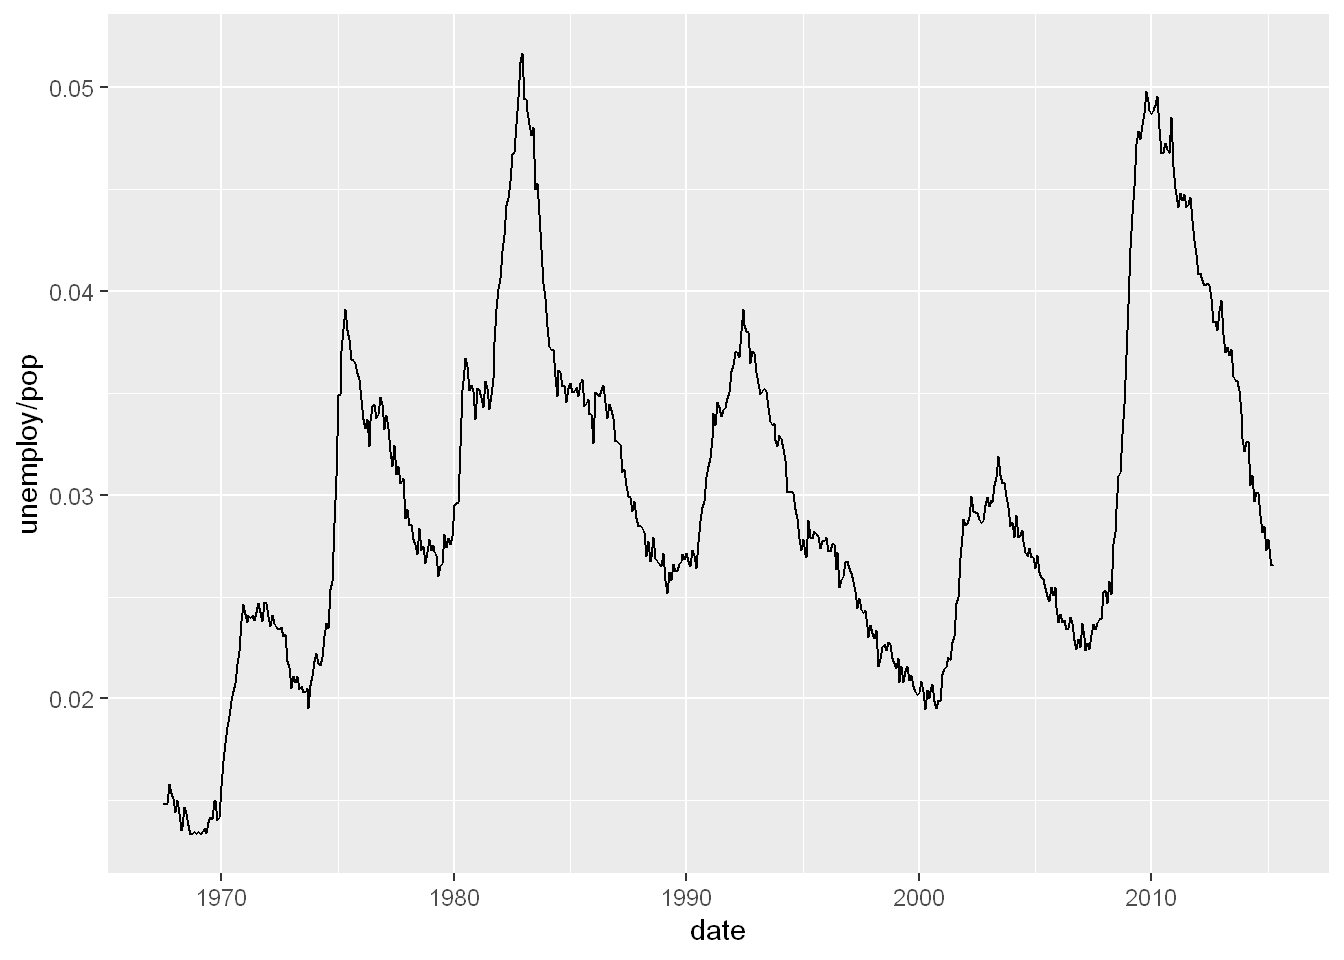
\includegraphics{09-GGPlot_files/figure-latex/fig2-14a-1.pdf}
\caption{\label{fig:fig2-14a}Left pane of Figure 2.14}
\end{figure}

\begin{Shaded}
\begin{Highlighting}[]
\NormalTok{fig2}\FloatTok{.14}\NormalTok{a }\SpecialCharTok{\%\textgreater{}\%} \FunctionTok{VI}\NormalTok{()   }
\end{Highlighting}
\end{Shaded}

\begin{verbatim}
This is an untitled chart with no subtitle or caption.
It has x-axis 'date' with labels 1960, 1970, 1980, 1990, 2000, 2010 and 2020.
It has y-axis 'unemploy/pop' with labels 0.02, 0.03, 0.04 and 0.05.
The chart is a set of 1 line.
Line 1 connects 574 points.
\end{verbatim}

\hypertarget{path-plots}{%
\section{Path plots}\label{path-plots}}

\begin{Shaded}
\begin{Highlighting}[]
\NormalTok{year }\OtherTok{\textless{}{-}} \ControlFlowTok{function}\NormalTok{(x) }\FunctionTok{as.POSIXlt}\NormalTok{(x)}\SpecialCharTok{$}\NormalTok{year }\SpecialCharTok{+} \DecValTok{1900}    
\NormalTok{fig2}\FloatTok{.15}\NormalTok{b }\OtherTok{=} \FunctionTok{qplot}\NormalTok{(unemploy }\SpecialCharTok{/}\NormalTok{ pop, uempmed, }\AttributeTok{data =}\NormalTok{ economics, }\AttributeTok{geom =} \StringTok{"path"}\NormalTok{, }\AttributeTok{colour=}\FunctionTok{year}\NormalTok{(date)) }
\CommentTok{\#+ scale\_area() \# no longer works}
\NormalTok{fig2}\FloatTok{.15}\NormalTok{b}
\end{Highlighting}
\end{Shaded}

\begin{figure}
\centering
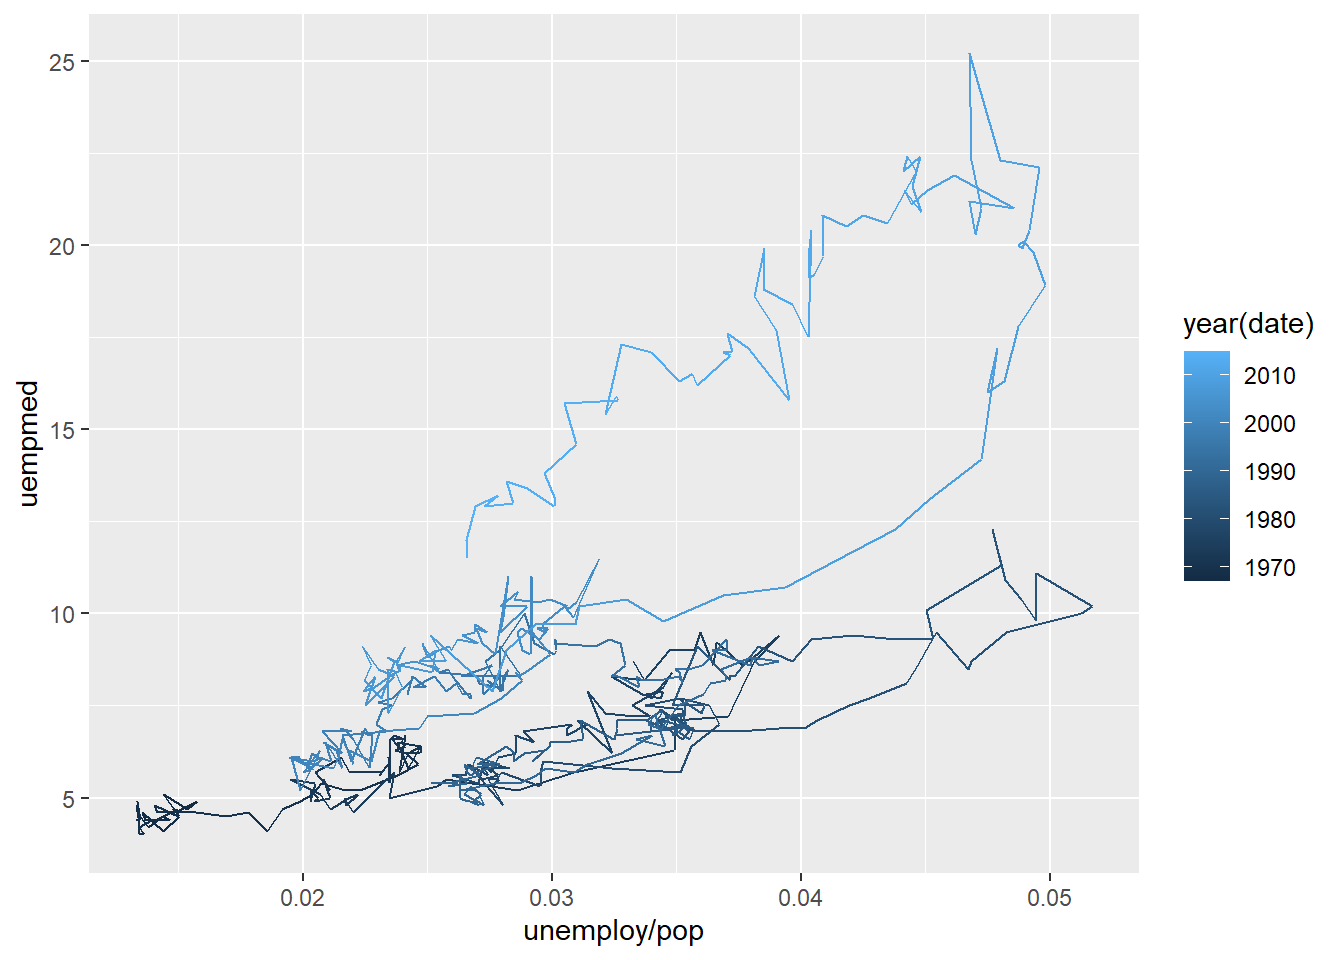
\includegraphics{09-GGPlot_files/figure-latex/fig2-15b-1.pdf}
\caption{\label{fig:fig2-15b}Right pane of Figure 2.15}
\end{figure}

\begin{Shaded}
\begin{Highlighting}[]
\NormalTok{fig2}\FloatTok{.15}\NormalTok{b }\SpecialCharTok{\%\textgreater{}\%} \FunctionTok{VI}\NormalTok{()   }
\end{Highlighting}
\end{Shaded}

\begin{verbatim}
This is an untitled chart with no subtitle or caption.
It has x-axis 'unemploy/pop' with labels 0.02, 0.03, 0.04 and 0.05.
It has y-axis 'uempmed' with labels 5, 10, 15, 20 and 25.
There is a legend indicating colour is used to show year(date), ranging from 1967 represented by colour dark purplish blue to 2015 shown as colour brilliant blue.
The chart is a path graph that VI can not process.
\end{verbatim}

\hypertarget{facets-is-the-ggplot-term-for-trellis-panels}{%
\section{Facets is the ggplot term for trellis' panels}\label{facets-is-the-ggplot-term-for-trellis-panels}}

The aspect ratio for the plot region is something that needs to be considered. I've manually adjusted the plotting window here so that the graph more closely matches that of \citet{Wickham2009ggplot2} but it is not an exact match.

\begin{Shaded}
\begin{Highlighting}[]
\NormalTok{fig2}\FloatTok{.16}\NormalTok{a }\OtherTok{=} \FunctionTok{qplot}\NormalTok{(carat, }\AttributeTok{data =}\NormalTok{ diamonds, }\AttributeTok{facets =}\NormalTok{ color }\SpecialCharTok{\textasciitilde{}}\NormalTok{ ., }\AttributeTok{geom =} \StringTok{"histogram"}\NormalTok{, }\AttributeTok{binwidth =} \FloatTok{0.1}\NormalTok{, }
\AttributeTok{xlim =} \FunctionTok{c}\NormalTok{(}\DecValTok{0}\NormalTok{, }\DecValTok{3}\NormalTok{))    }
\NormalTok{fig2}\FloatTok{.16}\NormalTok{a}
\end{Highlighting}
\end{Shaded}

\begin{verbatim}
Warning: Removed 32 rows containing non-finite values (stat_bin).
\end{verbatim}

\begin{verbatim}
Warning: Removed 14 rows containing missing values (geom_bar).
\end{verbatim}

\begin{figure}
\centering
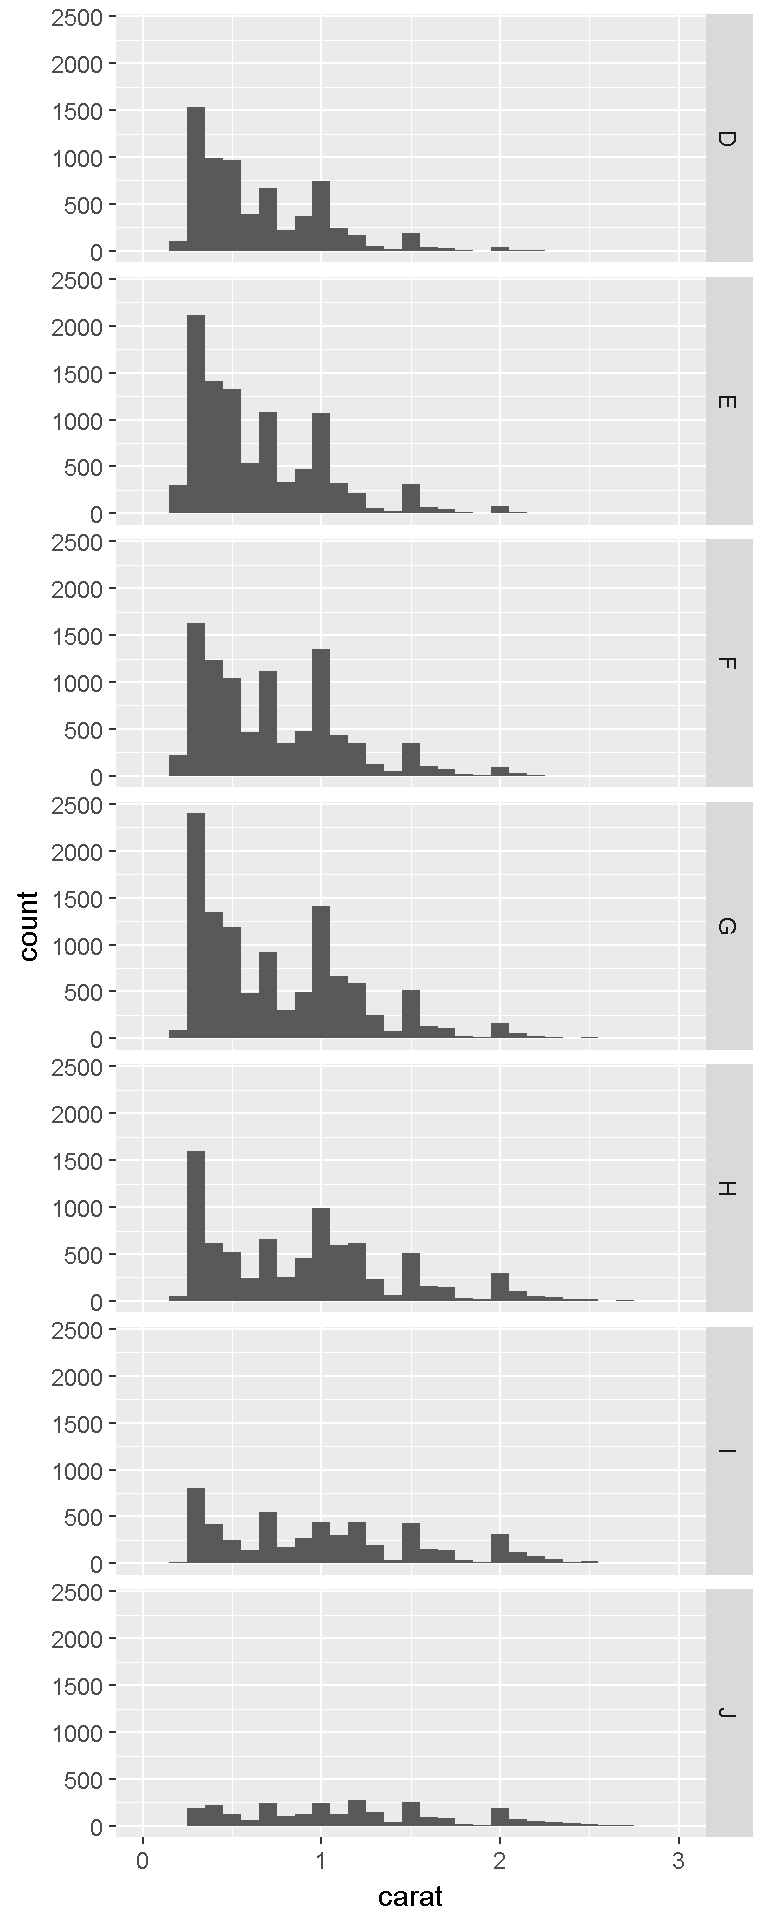
\includegraphics{09-GGPlot_files/figure-latex/fig2-16a-1.pdf}
\caption{\label{fig:fig2-16a}Left side of Figure 2.16}
\end{figure}

\begin{Shaded}
\begin{Highlighting}[]
\NormalTok{fig2}\FloatTok{.16}\NormalTok{a }\SpecialCharTok{\%\textgreater{}\%} \FunctionTok{VI}\NormalTok{()   }
\end{Highlighting}
\end{Shaded}

\begin{verbatim}
Warning: Removed 32 rows containing non-finite values (stat_bin).
\end{verbatim}

\begin{verbatim}
This is an untitled chart with no subtitle or caption.
The chart is comprised of 7 panels containing sub-charts, arranged vertically.
The panels represent different values of color.
Each sub-chart has x-axis 'carat' with labels 0, 1, 2 and 3.
Each sub-chart has y-axis '' with labels 0, 500, 1000, 1500, 2000 and 2500.
Panel 1 represents data for color = D.
Panel 1 is a bar chart with 29 vertical bars.
Panel 2 represents data for color = E.
Panel 2 is a bar chart with 29 vertical bars.
Panel 3 represents data for color = F.
Panel 3 is a bar chart with 29 vertical bars.
Panel 4 represents data for color = G.
Panel 4 is a bar chart with 29 vertical bars.
Panel 5 represents data for color = H.
Panel 5 is a bar chart with 29 vertical bars.
Panel 6 represents data for color = I.
Panel 6 is a bar chart with 29 vertical bars.
Panel 7 represents data for color = J.
Panel 7 is a bar chart with 29 vertical bars.
\end{verbatim}

\begin{Shaded}
\begin{Highlighting}[]
\NormalTok{fig2}\FloatTok{.16}\NormalTok{b }\OtherTok{=} \FunctionTok{qplot}\NormalTok{(carat, ..density.., }\AttributeTok{data =}\NormalTok{ diamonds, }\AttributeTok{facets =}\NormalTok{ color }\SpecialCharTok{\textasciitilde{}}\NormalTok{ ., }\AttributeTok{geom =} \StringTok{"histogram"}\NormalTok{, }\AttributeTok{binwidth =} \FloatTok{0.1}\NormalTok{, }\AttributeTok{xlim =} \FunctionTok{c}\NormalTok{(}\DecValTok{0}\NormalTok{, }\DecValTok{3}\NormalTok{))   }
\NormalTok{fig2}\FloatTok{.16}\NormalTok{b}
\end{Highlighting}
\end{Shaded}

\begin{verbatim}
Warning: Removed 32 rows containing non-finite values (stat_bin).
\end{verbatim}

\begin{verbatim}
Warning: Removed 14 rows containing missing values (geom_bar).
\end{verbatim}

\begin{figure}
\centering
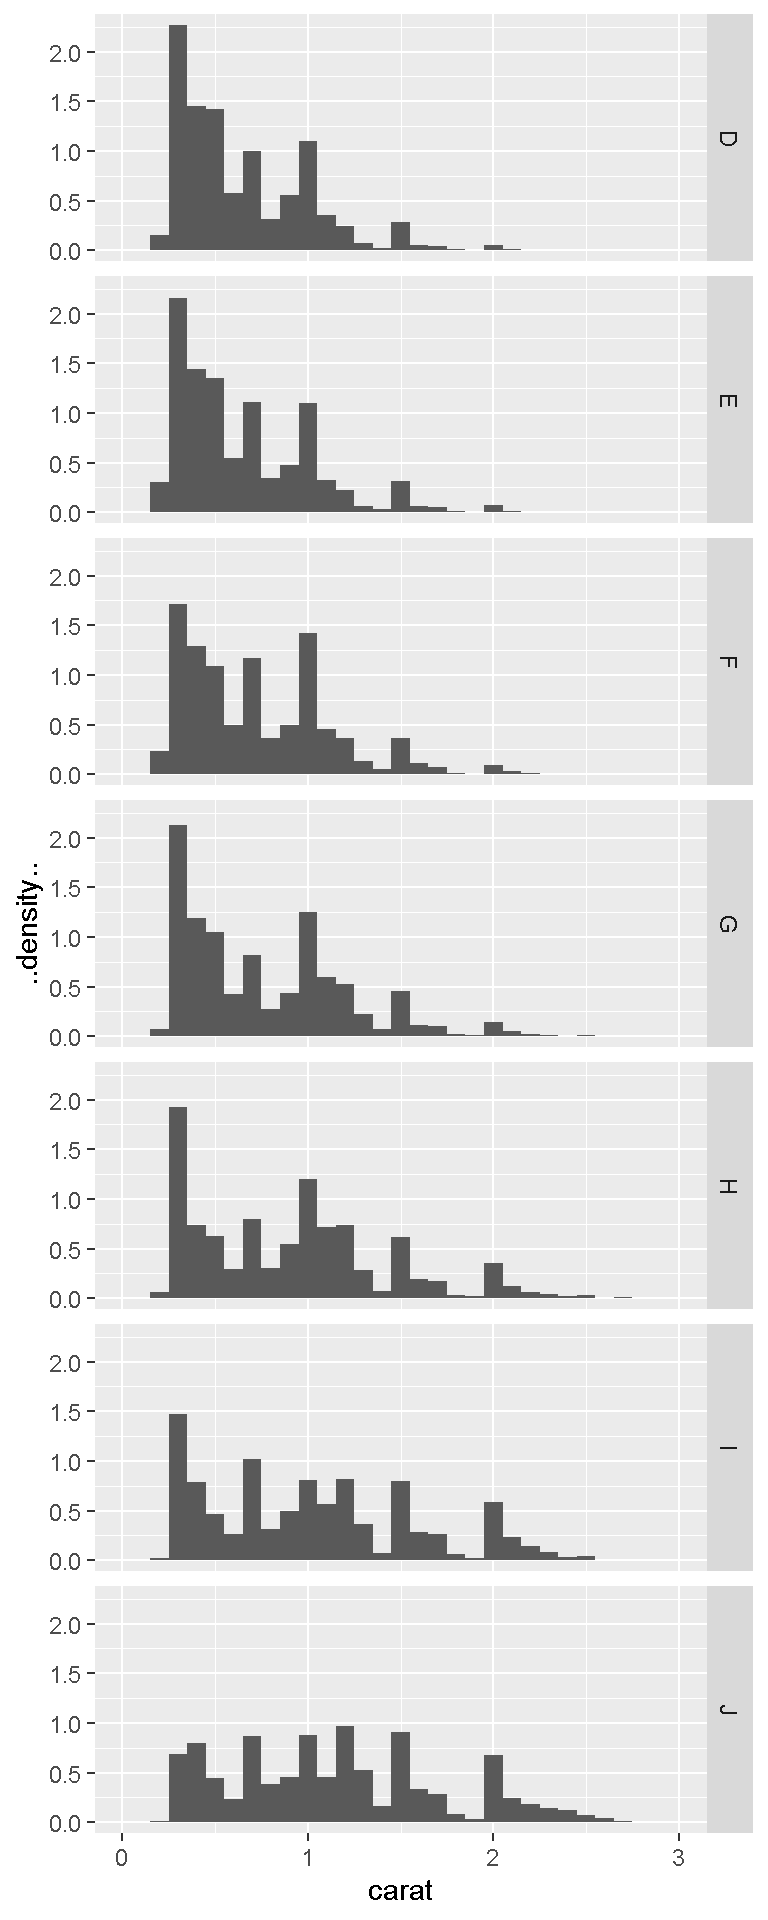
\includegraphics{09-GGPlot_files/figure-latex/fig2-16b-1.pdf}
\caption{\label{fig:fig2-16b}Right side of Figure 2.16}
\end{figure}

\begin{Shaded}
\begin{Highlighting}[]
\NormalTok{fig2}\FloatTok{.16}\NormalTok{b }\SpecialCharTok{\%\textgreater{}\%} \FunctionTok{VI}\NormalTok{()   }
\end{Highlighting}
\end{Shaded}

\begin{verbatim}
Warning: Removed 32 rows containing non-finite values (stat_bin).
\end{verbatim}

\begin{verbatim}
This is an untitled chart with no subtitle or caption.
The chart is comprised of 7 panels containing sub-charts, arranged vertically.
The panels represent different values of color.
Each sub-chart has x-axis 'carat' with labels 0, 1, 2 and 3.
Each sub-chart has y-axis '..density..' with labels 0.0, 0.5, 1.0, 1.5 and 2.0.
Panel 1 represents data for color = D.
Panel 1 is a bar chart with 29 vertical bars.
Panel 2 represents data for color = E.
Panel 2 is a bar chart with 29 vertical bars.
Panel 3 represents data for color = F.
Panel 3 is a bar chart with 29 vertical bars.
Panel 4 represents data for color = G.
Panel 4 is a bar chart with 29 vertical bars.
Panel 5 represents data for color = H.
Panel 5 is a bar chart with 29 vertical bars.
Panel 6 represents data for color = I.
Panel 6 is a bar chart with 29 vertical bars.
Panel 7 represents data for color = J.
Panel 7 is a bar chart with 29 vertical bars.
\end{verbatim}

\hypertarget{rescaling-of-the-axes}{%
\section{Rescaling of the axes}\label{rescaling-of-the-axes}}

\begin{Shaded}
\begin{Highlighting}[]
\NormalTok{p26a }\OtherTok{=} \FunctionTok{qplot}\NormalTok{(carat, price, }\AttributeTok{data =}\NormalTok{ dsmall, }\AttributeTok{log =} \StringTok{"xy"}\NormalTok{)   }
\NormalTok{p26a}
\end{Highlighting}
\end{Shaded}

\begin{figure}
\centering
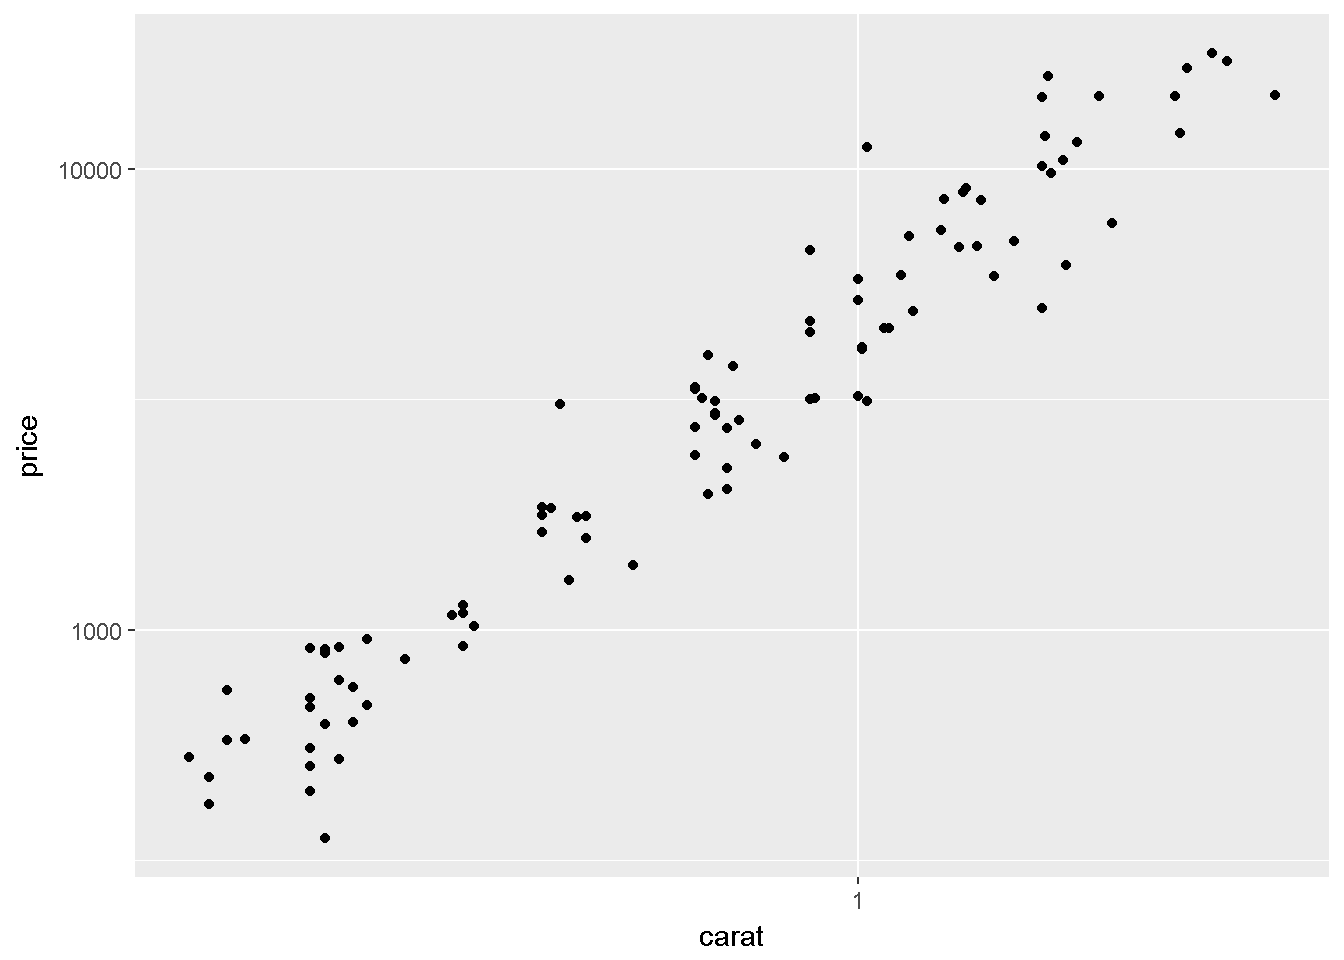
\includegraphics{09-GGPlot_files/figure-latex/p26a-1.pdf}
\caption{\label{fig:p26a}First graph on page 26 of}
\end{figure}

\begin{Shaded}
\begin{Highlighting}[]
\NormalTok{p26a }\SpecialCharTok{\%\textgreater{}\%} \FunctionTok{VI}\NormalTok{()   }
\end{Highlighting}
\end{Shaded}

\begin{verbatim}
This is an untitled chart with no subtitle or caption.
It has x-axis 'carat' with labels 0.3, 1.0 and 3.0.
It has y-axis 'price' with labels 1000, 3000 and 10000.
The chart is a set of 100 points.
\end{verbatim}

\begin{Shaded}
\begin{Highlighting}[]
\NormalTok{fig3}\FloatTok{.6} \OtherTok{=} \FunctionTok{qplot}\NormalTok{(displ, hwy, }\AttributeTok{data=}\NormalTok{mpg, }\AttributeTok{facets =}\SpecialCharTok{\textasciitilde{}}\NormalTok{ year) }\SpecialCharTok{+} \FunctionTok{geom\_smooth}\NormalTok{()    }
\NormalTok{fig3}\FloatTok{.6}
\end{Highlighting}
\end{Shaded}

\begin{verbatim}
`geom_smooth()` using method = 'loess' and formula 'y ~ x'
\end{verbatim}

\begin{figure}
\centering
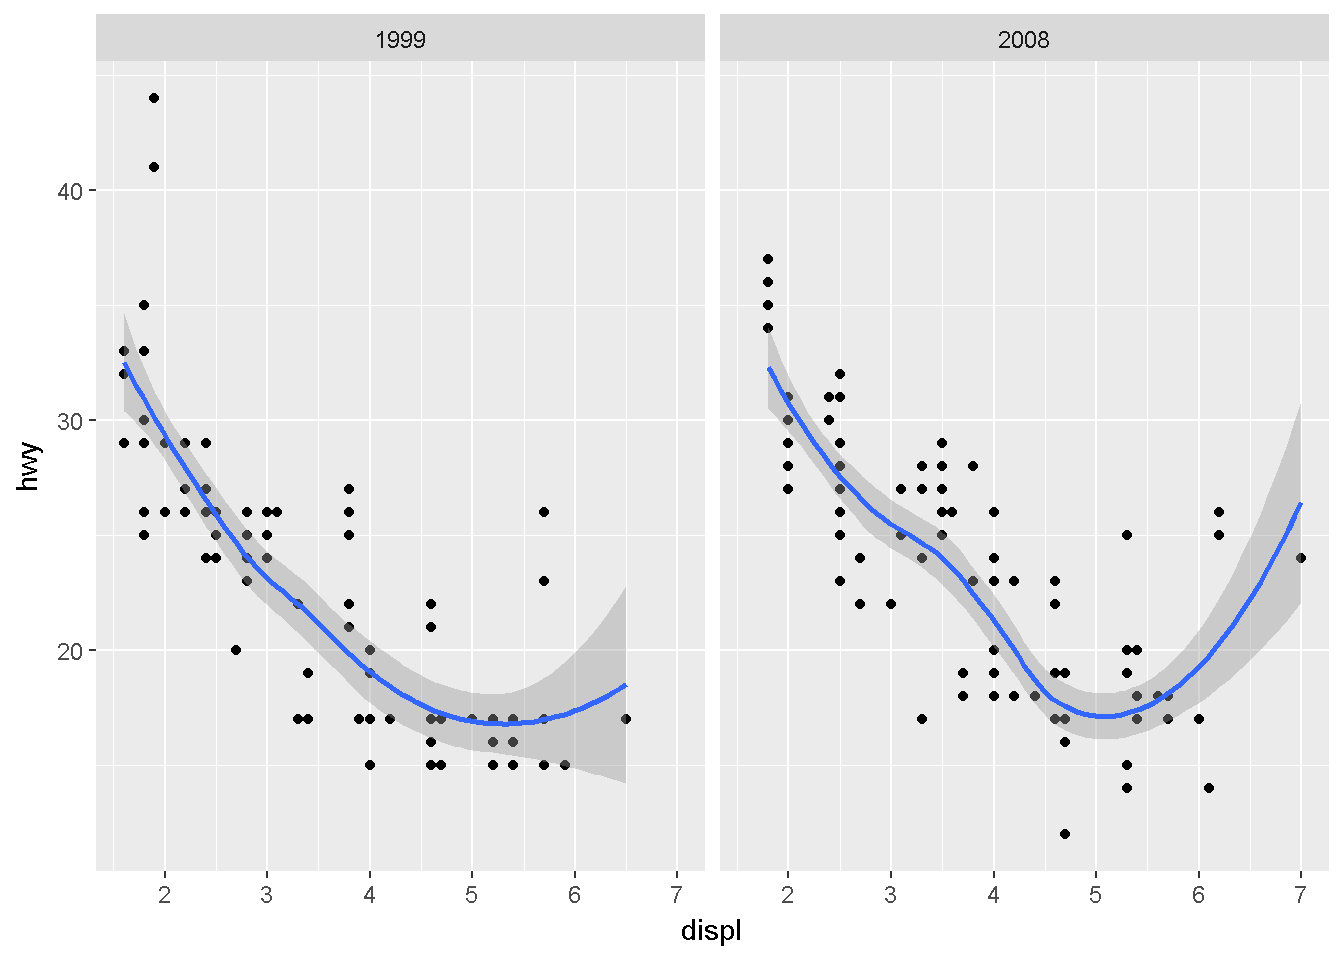
\includegraphics{09-GGPlot_files/figure-latex/fig3-6-1.pdf}
\caption{\label{fig:fig3-6}Figure 3.6 of}
\end{figure}

\begin{Shaded}
\begin{Highlighting}[]
\NormalTok{fig3}\FloatTok{.6} \SpecialCharTok{\%\textgreater{}\%} \FunctionTok{VI}\NormalTok{()   }
\end{Highlighting}
\end{Shaded}

\begin{verbatim}
This is an untitled chart with no subtitle or caption.
The chart is comprised of 2 panels containing sub-charts, arranged horizontally.
The panels represent different values of year.
Each sub-chart has x-axis 'displ' with labels 2, 3, 4, 5, 6 and 7.
Each sub-chart has y-axis 'hwy' with labels 20, 30 and 40.
Each sub-chart has 2 layers.
Panel 1 represents data for year = 1999.
Layer 1 of panel 1 is a set of 117 points.
Layer 2 of panel 1 is a 'lowess' smoothed curve with 95% confidence intervals.Panel 2 represents data for year = 2008.
Layer 1 of panel 2 is a set of 117 points.
Layer 2 of panel 2 is a 'lowess' smoothed curve with 95% confidence intervals.
\end{verbatim}

\hypertarget{WriteR}{%
\chapter{Getting started with the WriteR application}\label{WriteR}}

The WriteR application was written to support use of R markdown and the \texttt{BrailleR} package. It is a Python script making use of wxPython to help build the graphic user interface (GUI) in such a way that it works for screen reader users. This book has been written in R markdown, and I have made extensive use of WriteR because it offers so many convenient tools for a blind user wanting to write R markdown files.

The script is in the \texttt{BrailleR} package, but it cannot run unless the user has both Python and wxPython installed. Commands have been included in the \texttt{BrailleR} package to help Windows users obtain installation files for them. Users of other operating systems currently have to install Pandoc, Python and wxPython independently, but these tools may well already be installed.

\hypertarget{getting-the-required-software-windows-users-only}{%
\section{Getting the required software (Windows users only)}\label{getting-the-required-software-windows-users-only}}

You can check if a version of Python is already installed on your computer using

\begin{Shaded}
\begin{Highlighting}[]
\FunctionTok{Sys.which}\NormalTok{(}\StringTok{"Python"}\NormalTok{)}
\end{Highlighting}
\end{Shaded}

\begin{verbatim}
                              Python 
"C:\\PROGRA~1\\Python38\\Python.exe" 
\end{verbatim}

The output above shows you that I have Python 3.8 installed on my computer, and that it can be found in the folder I know is the default location. You can use this command later to check your progress, but there are other ways to check your system that return more useful detail, but for the moment the \texttt{Sys.which()} command above issufficient. What it does not show you is whether the installation of Python is suited for a 64 bit machine, or is the more universal 32 bit installation. We really ought to have an exact match between the version of Python and the version of R being used.

The files downloaded as a consequence of running commands in this set of instructions will be saved in your \texttt{MyBrailleR} folder. You will need to follow the instructions and answer questions that arise whenever you install new software, but you should probably read all the way through this set of instructions before getting underway.

Ultimately, you will need a mainstream tool to process the markdown files you write into other formats. The WriteR application will end up using a tool called ``pandoc'' to do this so we need to get this installed.
If you do not have an installation of Pandoc and Python 3 then you can use some functions from the \texttt{BrailleR} package to help make the setup smoother. Remember to load the package using:

\texttt{library(BrailleR)}

It doesn't matter if you install Python before or after Pandoc.

\hypertarget{installing-pandoc}{%
\subsection{Installing Pandoc}\label{installing-pandoc}}

Let's first install Pandoc using the command:

\texttt{GetPandoc()}

To check that you have Pandoc installed, and that R can therefore find it, use the command"

\begin{Shaded}
\begin{Highlighting}[]
\FunctionTok{Sys.which}\NormalTok{(}\StringTok{"pandoc"}\NormalTok{)}
\end{Highlighting}
\end{Shaded}

\begin{verbatim}
                            pandoc 
"C:\\PROGRA~1\\Pandoc\\pandoc.exe" 
\end{verbatim}

which will show where Pandoc was installed.

\hypertarget{installing-python}{%
\subsection{Installing Python}\label{installing-python}}

The following instructions fetch the installation files from the reputable Python sites. Windows and any security software you might have should know that, but you can never tell! You may need to let Windows know it is OK to install the software in the default location. The pop-up might not appear as the window with focus so if things look like they're going slowly, look around for the pop-up window.

The following commands automatically download the installation files needed for Python 3.x, and start the installation process going.
Issue them at the R prompt

\texttt{GetPython3()}

Make sure that the first thing you do as part of the installation is to choose to use a custom installation. This allows you to make sure Python will be availabel to all users, update the system's environment variables. You may need to make sure these options are selected.

You need to make sure that the second of these options definitely happens; this ensures that the Python folders are added to your system path which means R and any other software that wants Python can find it. This makes it possible to run Python scripts from any folder on your computer. The next few commands will fail if this is not done properly. If you missed that step during the installation, look for the installer file in your \texttt{MyBrailleR} folder and run it again manually before proceeding.

We can check the installation has worked properly at this point using:

\begin{Shaded}
\begin{Highlighting}[]
\FunctionTok{Sys.which}\NormalTok{(}\StringTok{"python"}\NormalTok{)}
\end{Highlighting}
\end{Shaded}

\begin{verbatim}
                              python 
"C:\\PROGRA~1\\Python38\\python.exe" 
\end{verbatim}

\begin{Shaded}
\begin{Highlighting}[]
\FunctionTok{shell}\NormalTok{(}\StringTok{"path"}\NormalTok{, }\AttributeTok{intern=}\ConstantTok{TRUE}\NormalTok{)}
\end{Highlighting}
\end{Shaded}

\begin{verbatim}
[1] "PATH=C:\\Program Files\\Python38\\Scripts\\;C:\\Program Files\\Python38\\;C:\\Rtools\\bin;C:\\Program Files\\ImageMagick-7.0.7-Q16;C:\\WINDOWS\\system32;C:\\WINDOWS;C:\\WINDOWS\\System32\\Wbem;C:\\WINDOWS\\System32\\WindowsPowerShell\\v1.0\\;C:\\Program Files\\Intel\\WiFi\\bin\\;C:\\Program Files\\Common Files\\Intel\\WirelessCommon\\;C:\\Program Files\\MiKTeX 2.9\\miktex\\bin\\x64\\;C:\\Program Files (x86)\\Pandoc\\;c:\\batch;C:\\Program Files\\Git\\cmd;C:\\Program Files\\Git\\mingw64\\bin;C:\\Program Files\\Git\\usr\\bin;C:\\WINDOWS\\System32\\OpenSSH\\;C:\\Program Files (x86)\\Intel\\Intel(R) Management Engine Components\\DAL;C:\\Program Files\\Intel\\Intel(R) Management Engine Components\\DAL;C:\\Program Files\\Pandoc\\;C:\\Users\\ajgodfre\\AppData\\Local\\Microsoft\\WindowsApps;"
\end{verbatim}

This is a much stronger test than was done earlier. You can see the folders that Windows will search through to find the tools you are using all the time. The folder for Python needs to be listed there somewhere.

Now get the additional Python modules needed for WriteR using:

\texttt{GetWxPython3()}

Once you have completed these installations, you are ready to go. You shouldn't need to keep the installation files, but why not keep them just in case.
You can now skip to the section which shows you how to check everything is ready for using WriteR.

\hypertarget{other-operating-systems}{%
\section{Other operating systems}\label{other-operating-systems}}

\hypertarget{checking-your-system-is-ready}{%
\section{Checking your system is ready}\label{checking-your-system-is-ready}}

All going to plan, you should now have Python on your system, and the additional wxPython module as well. You only need to check that R really can see the right version of Python, and that one extra Python module is correctly installed and available to R to find out how well you've done, using:

\begin{Shaded}
\begin{Highlighting}[]
\FunctionTok{TestWX}\NormalTok{()}
\end{Highlighting}
\end{Shaded}

\begin{verbatim}
Your system is using Python 3.8.0
\end{verbatim}

\begin{verbatim}
Python can see the necessary wx module.
You are ready to use WriteR.
\end{verbatim}

N.B. The command will return more output on your system if you test the function in an interactive setting. Do that now.

The outcome of this command tells you if your system is ready to run the WriteR application. It first checks that a version of Python is available, and if there is, then runs a short script that uses WxPython.

If you are in an interactive session, and Python is all working, then a small window will have opened on your system, and told you that you are ready to use WriteR.

If for some reason you are not getting it all going properly, then there are several commands that can be issued at a command prompt. Windows users get a command prompt by typing \texttt{cmd} at the \texttt{Run} (Found by \texttt{Windows+R}).

The following commands are not R commands. They should work on all operating systems. Do not proceed until each has worked without error messages.

1.Typing

\begin{verbatim}
python --version
\end{verbatim}

will tell you if Python is installed by returning the version number.
2. Make sure you can use the tool that grabs extra Python modules from an official site by typing

\begin{verbatim}
pip --version
\end{verbatim}

If this doesn't work you will need to seek out the correct strategy via the Python wiki pages available online.
3. Upgrade your Python modules using

\begin{verbatim}
python -m pip install --user --upgrade pip setuptools wheel
\end{verbatim}

This should download a few files and automatically put them on your system.
4. Finnally, install the wxPython module using

\begin{verbatim}
pip install --user --upgrade wxPython
\end{verbatim}

Remember, do not move on to the next step until each of the commands above has returned satisfactory feedback. Windows users close the window using \texttt{Alt+F4} or by typing \texttt{exit}.

I strongly recommend that you go back and check everything has worked using the commands presented earlier in this chapter.

\hypertarget{opening-writer-from-brailler}{%
\section{Opening WriteR from BrailleR}\label{opening-writer-from-brailler}}

Opening WriteR is as easy as typing WriteR! Well almost. You have the option of specifying a filename; if that file exists, it gets opened for you, and if it doesn't exist, then it gets created with a few lines already included at the top to help get you started. Try:

\texttt{WriteR("MyFirst.Rmd")}

This should open the WriteR application with the following lines already there for you to edit.

\begin{verbatim}
---
title: ""
author: ""
date: ""
output:
    html_document:
        toc: false
        number_sections: false
        fig_height: 5
        fig_width: 7
--- 
\end{verbatim}

Some of these lines were explained back in Chapter \ref{WorkingBlind}. Fill in the gaps in the first few lines for title, author, and the date before continuing.

\hypertarget{what-can-i-do-with-writer}{%
\section{What can I do with WriteR?}\label{what-can-i-do-with-writer}}

The window you are in has a number of menus, a status bar at the bottom and a big space in the middle for your work. Take a quick look at those menus; some will look familiar because they are common to many Windows applications.

The file you have opened is a markdown file. It is just text which is why it is so easy to read. The file extension of \texttt{Rmd} means it is an R markdown file. There are several flavours of markdown in common use, but they are practically all the same except for some very minor differences.

A markdown file can be converted into many file formats for distribution. These include HTML, pdf, Microsoft Word, Open Office, and a number of different slide presentation formats. Let's make the HTML file now.

\hypertarget{our-first-html-file}{%
\section{Our first HTML file}\label{our-first-html-file}}

Making your first HTML file is as easy as hitting the \texttt{f5} key, or using one of the options in the \texttt{Build} menu. The variety of options are the commonly used ones in RStudio. Let's just stick to making an HTML file for the time being. You can investigate other formats later.

When the processing is underway, a second window will open which gives the same output that you would see printed in an R session window if you were processing R markdown files manually.
If the last line says ``done 0'', then everything processed properly; if it says ``done 1'' then there was an error to fix, so look through this log to see what went wrong.

The processing of your R markdown document will use a suite of packages, primarily including the \texttt{knitr} \citep{Rpkg-knitr} and \texttt{rmarkdown} \citep{Rpkg-rmarkdown} packages.
Press the \texttt{f4} key to switch back to the main document editing window in WriteR.

If the processing of the file ``MyFirst.Rmd'' was successful, then you will now have a file called ``MyFirst.html'' in your current working directory. You have several choices for finding the HTML file you have created:

\begin{itemize}
\tightlist
\item
  Navigate to the current working directory using your file browser. To find out where that is, type \texttt{getwd()} in the R window to see where the files really are located, or if you are a Windows user, issue the \texttt{BrailleR} function \texttt{Explorer()} to opent he folder automatically.
  You should see the file \texttt{MyFirst.Rmd} and once you have built it, the associated HTML file. Open that file in your browser.
\item
  Use the \texttt{browseURL()} command in the R session. You will need to provide the filename, in quotes, for example \texttt{browseURL("MyFirst.html")}
\end{itemize}

Use one of these methods to open the HTML file. Read through it to see how the markdown has been rendered.
You may need to switch back and forth between the WriteR window and your browser to compare the plain text and the beautiful HTML. If you didn't actually edit the R markdown file up to now then the output HTML file will be rather boring. Add in some text, or use the menus to see how to insert headings and other things.

N.B. Changes in your R markdown file are not automatically converted into the HTML file. You must re-build the HTML, and refresh your browser to see the impact of any changes you make, both actions use the \texttt{f5} key.

\hypertarget{some-hints-for-writing-rmarkdown-documents}{%
\section{Some hints for writing Rmarkdown documents}\label{some-hints-for-writing-rmarkdown-documents}}

The WriteR application really can make writing documents easier because it offers plenty of shortcut keystrokes for items in the pulldown menus. Formatting text in a markdown document which will be converted to HTML is done in a way that creates semantic structure at the same time as font changes, or to put more precisely, you can't get a larger font for a heading without using a proper heading style. My list of hints given here are to help make your final HTML document a pleasure to read as well as easy to write.

\begin{itemize}
\tightlist
\item
  Always use the standard markdown syntax for inserting headings, graphics, links, and equations. WriteR will insert placeholders for graphics and links and some mathematical structures.
\item
  Concentrate on the material to be communicated; do not worry about the formatting of it. Keeping it simple is best.
\item
  Make use of the lessons learned by others. If you like hte way something is presented, then re-use the approach taken.
\item
  if you inset a graph created in an R chunk, then make sure you use the \texttt{fig.cap} properly. This text will be used as the ``alt tag'' for the resulting graph.
\item
  One figure per chunk is recommended. This helps with the alt tags.
\item
  The default presentation of R output is to have three hash signs at the left of each line of output. Inclusion of an R chunk at the start of the document can fix this. Use something like:
\end{itemize}

\begin{verbatim}
```r
library(knitr)
opts_chunk$set(comment="")
```
\end{verbatim}

I found the flow of some documents was unnecessarily clunky when simple mathematical elements were entered as math mode elements. Sentences will read better if \emph{x} and \emph{y} are in italicised font and not math mode, and the sighted readers won't notice the difference. This won't work for Greek, some subscripts and superscripts, or symbols. If in doubt, use math mode everywhere. This means using a dollar on both sides of the mathematical content such as \texttt{\$x\$} for example.

The method used to convert your raw markdown to beautiful HTML will matter. WriteR has been configured to use \texttt{render()} from the \texttt{rmarkdown} package as it delivers the best outcome for screen reader users.

Finally, you should investigate which combination of screen reader and browser gives you the results you like best. I regularly make use of both JAWS and NVDA, and my preferred browser has changed over the years. I used to only ever use Firefox, but Chrome gets more use today; both Internet Explorer and Opera have both been used at times.

\hypertarget{brailler-commands-used-in-this-chapter-6}{%
\section{BrailleR commands used in this chapter}\label{brailler-commands-used-in-this-chapter-6}}

We used \texttt{TestWX()} to check the necessary Python installations were successful. It automatically called the \texttt{TestPython()} command as its first step.

We needed to use \texttt{GetPython3()} and \texttt{GetWxPython3()} to install the necessary software to run a Python script like WriteR.

Finally, we opened a new file using \texttt{WriteR()}.

\hypertarget{AccessibleGraphs}{%
\chapter{Making Accessible Graphs}\label{AccessibleGraphs}}

While the initial aim of the BrailleR Project was to create a text description of a graph, there are many ways to explore graphs created in R by other means. This chapter introduces some techniques for creating or modifying graphs so that they can be investigated by a blind person without the assistance of a sighted person.

\hypertarget{LookingAhead}{%
\chapter{The Work Ahead}\label{LookingAhead}}

The \texttt{BrailleR} Project is likely to evolve over time. The work on the project will be dependent on interest being shown by blind users of R, and perhaps some willingness being shown by people who could make the work so much easier.

Developments that meet specific requests from blind users are being addressed. For example, the request from one user to have the \texttt{BrailleR} package loaded in every session led to creation of a \texttt{MakeRprofile()} function; this function simplifies the experience for the user (a novice) for creation of the \texttt{.Rprofile} file in the current working directory. This is easier to explain to a novice than the process of altering the \texttt{.Rprofile} or \texttt{.Rprofile.site} files.

A request for assistance getting braille labels onto graphs has brought forward the plans to address this issue within the \texttt{BrailleR} package. The experimental \texttt{BRLThis()} function has been included in the package, as well as a similar \texttt{SVGThis()} function to optimise the settings for creation of a version using a braille font and a structured SVG file for a graph. The \texttt{BRLThis()} function creates a pdf document that has been successfully embossed on two different models of embosser, while SVG files generated by the \texttt{SVGThis()} function have only the bare minimum of useful content at this stage.

It may prove necessary for the \texttt{BRLThis()} function to be converted to a method like the \texttt{SVGThis()} functions so that the best results can be created for different graph types. At present, the \texttt{SVGThis()} is reliant on the existence of the \texttt{hist()} and \texttt{boxplot()} commands within the \texttt{BrailleR} package that are wrappers to the \texttt{graphics} package functions of the same name.
It is my hope that I can encourage the R development core team to create more classes. The additions are almost trivial from their perspective, but the workload for me as a programmer will reduce markedly if I can write simpler code to interpret the graphs. Knowing what type of graph has been created by an object rather than writing code that makes a reasonable attempt at guessing what type of graph was created is a key example. To this end, it will prove easier to work with the graphs created by the \texttt{xyplot()} function from the \texttt{lattice} package than the standard \texttt{plot()} command.

I will also need feedback from students and users of R, and perhaps their lecturers, tutors, and teachers, to see which ideas are working well for blind users. At present, the attempts being made are based on my own experiences and desires; I wanted functions to convert an R script to an R markdown file and a similr function to convert the history of commands to an Rmd file. The \texttt{R2Rmd()} and \texttt{History2Rmd()} functions were duly created; they have proven very useful in my work. I can only hoep others find them as useful. I am, therefore, seeking opportunities to share my work with blind users all over the world via a specially created email list for those people interested in how blind users can work with R\{\}. I believe that
adding perspectives is a crucial pathway for the project's development and all feedback is extremely welcome.

A key contribution is possible in the area of choosing appropriate default text for the \texttt{BrailleR} output. The text representation needs to be more efficient than using R in its vanilla form. To this end, I have put some time into thinking about which text will be most suitable for an audience that will often listen to the output using synthetic speech, perhaps in the user's second language, as well as the braille readers who may or may not be able to use contracted English braille. At first, I had thought this task would be made easier by reviewing resources created by transcribers who record books for the blind, but my investigations show that the descriptions used in spoken words do not always equate to efficient braille or synthetic speech and often provide more interpretation than I believe is appropriate in educational settings.

Collaboration from others in any role will feed my own enthusiasm for the project, especially those whose skills and knowledge complement my own.
The work of willing and helpful contributors has been gratefully received.
In some instances, other researchers in the R community have inadvertently contributed to \texttt{BrailleR} because I have been able to adapt their work to meet the needs of blind users.

\hypertarget{references}{%
\chapter{References}\label{references}}

  \bibliography{software.bib,Rpkgs.bib,book.bib,BrailleRPublications.bib,Access.bib,articles.bib,faulty.bib}

\end{document}
